
\section{Category theory}
\label{sec:cat}

In this section we review some category theory needed for this thesis. We will review the theory of monoidal category theory and its more refined cousins as well as some basic properties of limits as well as internal category theory.

\subsection{Monoidal categories and string diagrams}
\label{subsec:moncat}

In this subsection we review the basic theory of monoidal categories as well as their string diagrams. 

\begin{definition}
A {\bf monoidal category} is a category $\X$ equipped with a functor $\X\times\X\to \X$ called the {\bf tensor product}, equipped with a distiguished object $I$ of $\X$ called the {\bf tensor unit}; along with the following natural isomorphisms (given by components):

\begin{description}
\item[Left unitor:]
$$
u_X^L:I\otimes X \to X
$$
\item[Right unitor:]
$$
u_X^R: X\otimes I \to X
$$
\item[Associator:]
$$
\alpha_{X,Y,Z}:(X\otimes Y)\otimes Z \to X\otimes(Y\otimes Z)
$$
\end{description}

Satisfying the following coherence equations:

\begin{description}
\item[MacLane pentagon:]


$$
\xymatrix{
  ((W\otimes X )\otimes Y)\otimes Z \ar[rr]^{\alpha_{W\otimes X,Y,Z}} \ar[d]_{\alpha_{W,X,Y}\otimes 1_Z}
    &
    & (W\otimes X )\otimes (Y\otimes Z) \ar[d]^{\alpha_{W, X,Y\otimes Z}}
  \\  (W\otimes(X\otimes Y))\otimes Z \ar[dr]_{\alpha_{W,\otimes Y,Z}}
    & 
    & W\otimes (X\otimes(Y\otimes Z)) 
  \\&
    W\otimes ((X\otimes Y)\otimes Z) \ar[ur]_{1_W\otimes \alpha_{X,Y,Z}}
}
$$

\item[Unit triangle:]

$$
\xymatrix{
  (X\otimes I)\otimes Y \ar[rr]^{\alpha_{X,I,Y}} \ar[dr]_{u_X^{R}\otimes 1_Y}
    &
    & X\otimes (I\otimes Y) \ar[dl]^{1_X\otimes u_Y^{L}}\\
  & X\otimes Y
}
$$

\end{description}

If all of the components of the natural transformations are equalities, then the monoidal category is {\bf strict}.

Given two monoidal categories $\X$ and $\Y$ a (strong) {\bf monoidal functor} from $\X$ to $\Y$ is a functor $F:\X\to \Y$ together with an isomorphism $\epsilon:I^\X \to F(I^\X)$ and natural isomorphism with components $\mu_{X,Y}:F(X)\otimes^\Y F(Y) \to F(X \otimes^\X Y)$ such that the following coherence equations hold


$$
\xymatrix{
 (F(X)\otimes^\Y F(Y))\otimes^\Y F(Z) \ar[rrr]^{\alpha_{F(X),F(Y),F(Z)}^{\Y}} \ar[d]_{\mu_{X,Y}\otimes^\Y F(Z)}
   &&& F(X) \otimes^\Y (F(Y)\otimes^\Y F(Z)) \ar[d]^{F(X)\otimes^\Y \mu_{Y,Z}}
 \\F(X\otimes^\X Y)\otimes^\Y F(Z) \ar[d]_{\mu_{X\otimes^\X Y,Z}}
   &&& F(X)\otimes^\Y F(Y\otimes^\X Z) \ar[d]_{\mu_{X,Y\otimes^\Y Z}}
 \\ F((X\otimes^\X Y) \otimes^\X Z) \ar[rrr]_{F(\alpha_{X,Y,Z}^\Y)}
   &&& F(X\otimes^\X (Y\otimes^\X Z))
}
$$

$$
\xymatrix{
 I^\Y \otimes^\Y F(X) \ar[rr]^{\epsilon \otimes^\Y F(X)} \ar[d]_{(u^L)^\Y_{F(X)}}
  &&  F(I^\X) \otimes^\Y F(X) \ar[d]^{\mu_{1^\X,X}}
\\F(X)
 & & F(I^\X\otimes^\X X) \ar[ll]_{F((u^L)^\X_{X} )}
}
$$


$$
\xymatrix{
  F(X)  \otimes^\Y I^\Y \ar[rr]^{ F(X)  \otimes^\Y \epsilon} \ar[d]_{(u^R)^\Y_{F(X)}}
  && F(X) \otimes^\Y    F(I^\X)  \ar[d]^{\mu_{X,1^\X}}
\\F(X)
 & & F(X \otimes^\X I^\X ) \ar[ll]_{F((u^R)^\X_{X} )}
}
$$


A {\bf strict monoidal functor} is a monoidal functor where $\epsilon$ and $\mu$ are the identity.


A {\bf monoidal natural transformation} between parallel monoidal functors $F,F':\X\to \Y$ is a natural transformation $\phi:F\to F'$ such that the following coherence equations hold:

$$
\xymatrix{
  F(X)\otimes^\Y F(Y) \ar[rr]^{\phi_X\otimes^\Y \phi_Y} \ar[d]_{\mu_{X,Y}}
   && F'(X)\otimes^\Y F'(Y) \ar[d]^{\mu'_{X,Y}}
 \\F'(X\otimes^\X Y) \ar[rr]_{\phi_{X\otimes^\X Y}}
   && F'(X\otimes^\X Y)
},
\hspace*{.5cm}
\xymatrix{
I^\Y \ar[dr]^{\eta'} \ar[d]_{\eta}
\\ F(I^\X) \ar[r]_{\phi_{I^\X}}
  &F'(I^\X)
}
$$

Monoidal categories, monoidal functors and monoidal natural transformations arrange themselves into the 2-category of monoidal categories. Likewise, strict monoidal categories, strict monoidal functors and monoidal natural transformations arrange themselves into the 2-category of strict monoidal categories.
\end{definition}

\begin{example}
Sets and functions is a monoidal category under both the product and under the coproduct.
Finite ordinals and functions are a strict monoidal under the same tensor product.

Sets and monotone functions is a monoidal category under the coproduct.
Finite ordinals and order preserving maps is also a monoidal category under the tensor product.


Given a field $k$, vector spaces over $k$ are monoidal with respect to the bilinear tensor product and the direct sum.
Matrices over $k$ are monoidal categories under both the bilinear tensor product and the direct sum.
\end{example}

Strict monoidal categories have a particularly concise graphical calculus, called {\bf string diagrams}.  A map $f:X_1\otimes \cdots X_n\to Y_1\otimes \cdots \otimes Y_n$ is drawn as a box with $n$ wires coming out of the bottom and $m$ wires coming out of the top, all being labelled by their respective objects, as follows:


$$
\begin{tikzpicture}
	\begin{pgfonlayer}{nodelayer}
		\node [style=map] (0) at (0, 3) {$f$};
		\node [style=none] (1) at (-0.75, 2.25) {};
		\node [style=none] (2) at (-0.25, 2.25) {};
		\node [style=none] (3) at (0.75, 2.25) {};
		\node [style=none] (4) at (-0.75, 2) {$X_1$};
		\node [style=none] (5) at (-0.25, 2) {$X_2$};
		\node [style=none] (6) at (0.75, 2) {$X_n$};
		\node [style=none] (7) at (0.25, 2.25) {$\cdots$};
		\node [style=none] (8) at (-0.75, 3.75) {};
		\node [style=none] (9) at (-0.25, 3.75) {};
		\node [style=none] (10) at (0.75, 3.75) {};
		\node [style=none] (11) at (-0.75, 4) {$Y_1$};
		\node [style=none] (12) at (-0.25, 4) {$Y_2$};
		\node [style=none] (13) at (0.75, 4) {$Y_m$};
		\node [style=none] (14) at (0.25, 3.75) {$\cdots$};
	\end{pgfonlayer}
	\begin{pgfonlayer}{edgelayer}
		\draw [in=90, out=-135, looseness=0.75] (0) to (1.center);
		\draw [in=255, out=90] (2.center) to (0);
		\draw [in=90, out=-45, looseness=0.75] (0) to (3.center);
		\draw [in=105, out=-90] (9.center) to (0);
		\draw [in=-90, out=135, looseness=0.75] (0) to (8.center);
		\draw [in=-90, out=45, looseness=0.75] (0) to (10.center);
	\end{pgfonlayer}
\end{tikzpicture}
$$


We often omit the objects when it is clear from context.  The tensor product of two maps $f:W_1\otimes W_n\to X_1\otimes \cdots \otimes X_m$ and $g:Y_1\otimes Y_k\to Z_1\otimes \cdots \otimes Z_\ell$,  $f\otimes g$ is given by pasting them side-by-side:


$$
\begin{tikzpicture}
	\begin{pgfonlayer}{nodelayer}
		\node [style=none] (79) at (20.25, 2.25) {};
		\node [style=none] (80) at (20.75, 2.25) {};
		\node [style=none] (81) at (21.75, 2.25) {};
		\node [style=none] (82) at (21.25, 2.25) {$\cdots$};
		\node [style=none] (83) at (20.25, 3.75) {};
		\node [style=none] (84) at (20.75, 3.75) {};
		\node [style=none] (85) at (21.75, 3.75) {};
		\node [style=none] (86) at (21.25, 3.75) {$\cdots$};
		\node [style=none] (87) at (22.25, 2.25) {};
		\node [style=none] (88) at (22.75, 2.25) {};
		\node [style=none] (89) at (23.75, 2.25) {};
		\node [style=none] (90) at (23.25, 2.25) {$\cdots$};
		\node [style=none] (91) at (22.25, 3.75) {};
		\node [style=none] (92) at (22.75, 3.75) {};
		\node [style=none] (93) at (23.75, 3.75) {};
		\node [style=none] (94) at (23.25, 3.75) {$\cdots$};
		\node [style=map] (95) at (22.1, 3) {\ $f\otimes g$\ \ };
		\node [style=none] (96) at (21.5, 3) {};
		\node [style=none] (97) at (21.75, 3) {};
		\node [style=none] (98) at (22, 3) {};
		\node [style=none] (99) at (22.25, 3) {};
		\node [style=none] (100) at (22.5, 3) {};
		\node [style=none] (101) at (22.75, 3) {};
		\node [style=none] (102) at (20.25, 2) {$W_1$};
		\node [style=none] (103) at (20.75, 2) {$W_2$};
		\node [style=none] (104) at (21.75, 2) {$W_m$};
		\node [style=none] (105) at (22.25, 2) {$Y_1$};
		\node [style=none] (106) at (22.75, 2) {$Y_2$};
		\node [style=none] (107) at (23.75, 2) {$Y_k$};
		\node [style=none] (108) at (20.25, 4) {$X_1$};
		\node [style=none] (109) at (20.75, 4) {$X_2$};
		\node [style=none] (110) at (21.75, 4) {$X_m$};
		\node [style=none] (111) at (22.25, 4) {$Z_1$};
		\node [style=none] (112) at (22.75, 4) {$Z_2$};
		\node [style=none] (113) at (23.75, 4) {$Z_\ell$};
	\end{pgfonlayer}
	\begin{pgfonlayer}{edgelayer}
		\draw [in=-90, out=90, looseness=0.50] (79.center) to (96.center);
		\draw [in=-90, out=90, looseness=0.50] (80.center) to (97.center);
		\draw [in=90, out=-90] (98.center) to (81.center);
		\draw (87.center) to (99.center);
		\draw [in=90, out=-90] (100.center) to (88.center);
		\draw [in=-90, out=90, looseness=0.75] (89.center) to (101.center);
		\draw [in=-90, out=90, looseness=0.75] (101.center) to (93.center);
		\draw [in=90, out=-90] (92.center) to (100.center);
		\draw (99.center) to (91.center);
		\draw [in=90, out=-90] (85.center) to (98.center);
		\draw [in=-90, out=90, looseness=0.50] (97.center) to (84.center);
		\draw [in=-90, out=90, looseness=0.50] (96.center) to (83.center);
	\end{pgfonlayer}
\end{tikzpicture}
:=
\begin{tikzpicture}
	\begin{pgfonlayer}{nodelayer}
		\node [style=map] (49) at (16.5, 3) {$f$};
		\node [style=none] (50) at (15.75, 2.25) {};
		\node [style=none] (51) at (16.25, 2.25) {};
		\node [style=none] (52) at (17.25, 2.25) {};
		\node [style=none] (53) at (16.75, 2.25) {$\cdots$};
		\node [style=none] (54) at (15.75, 3.75) {};
		\node [style=none] (55) at (16.25, 3.75) {};
		\node [style=none] (56) at (17.25, 3.75) {};
		\node [style=none] (57) at (16.75, 3.75) {$\cdots$};
		\node [style=map] (58) at (18.5, 3) {$g$};
		\node [style=none] (59) at (17.75, 2.25) {};
		\node [style=none] (60) at (18.25, 2.25) {};
		\node [style=none] (61) at (19.25, 2.25) {};
		\node [style=none] (62) at (18.75, 2.25) {$\cdots$};
		\node [style=none] (63) at (17.75, 3.75) {};
		\node [style=none] (64) at (18.25, 3.75) {};
		\node [style=none] (65) at (19.25, 3.75) {};
		\node [style=none] (66) at (18.75, 3.75) {$\cdots$};
		\node [style=none] (67) at (15.75, 4) {$X_1$};
		\node [style=none] (68) at (16.25, 4) {$X_2$};
		\node [style=none] (69) at (17.25, 4) {$X_m$};
		\node [style=none] (70) at (15.75, 2) {$W_1$};
		\node [style=none] (71) at (16.25, 2) {$W_2$};
		\node [style=none] (72) at (17.25, 2) {$W_m$};
		\node [style=none] (73) at (17.75, 2) {$Y_1$};
		\node [style=none] (74) at (18.25, 2) {$Y_2$};
		\node [style=none] (75) at (19.25, 2) {$Y_k$};
		\node [style=none] (76) at (17.75, 4) {$Z_1$};
		\node [style=none] (77) at (18.25, 4) {$Z_2$};
		\node [style=none] (78) at (19.25, 4) {$Z_\ell$};
	\end{pgfonlayer}
	\begin{pgfonlayer}{edgelayer}
		\draw [in=90, out=-135, looseness=0.75] (49) to (50.center);
		\draw [in=255, out=90] (51.center) to (49);
		\draw [in=90, out=-45, looseness=0.75] (49) to (52.center);
		\draw [in=105, out=-90] (55.center) to (49);
		\draw [in=-90, out=135, looseness=0.75] (49) to (54.center);
		\draw [in=-90, out=45, looseness=0.75] (49) to (56.center);
		\draw [in=90, out=-135, looseness=0.75] (58) to (59.center);
		\draw [in=255, out=90] (60.center) to (58);
		\draw [in=90, out=-45, looseness=0.75] (58) to (61.center);
		\draw [in=105, out=-90] (64.center) to (58);
		\draw [in=-90, out=135, looseness=0.75] (58) to (63.center);
		\draw [in=-90, out=45, looseness=0.75] (58) to (65.center);
	\end{pgfonlayer}
\end{tikzpicture}
$$

And a map $f:X_1\otimes X_n:\to Y_1\otimes \cdots \otimes Y_m$ is composed with a map $f:Y_1\otimes Y_m:\to Z_1\otimes \cdots \otimes Z_k$ by connecting the $Z_i$ togther:

$$
\begin{tikzpicture}
	\begin{pgfonlayer}{nodelayer}
		\node [style=none] (34) at (13.25, 2) {$X_1$};
		\node [style=none] (35) at (13.75, 2) {$X_2$};
		\node [style=none] (36) at (14.75, 2) {$X_n$};
		\node [style=none] (37) at (13.25, 4) {$Z_1$};
		\node [style=none] (38) at (13.75, 4) {$Z_2$};
		\node [style=none] (39) at (14.75, 4) {$Z_k$};
		\node [style=map] (40) at (14, 3) {$f;g$};
		\node [style=none] (41) at (13.25, 2.25) {};
		\node [style=none] (42) at (13.75, 2.25) {};
		\node [style=none] (43) at (14.75, 2.25) {};
		\node [style=none] (44) at (14.25, 2.25) {$\cdots$};
		\node [style=none] (45) at (13.25, 3.75) {};
		\node [style=none] (46) at (13.75, 3.75) {};
		\node [style=none] (47) at (14.75, 3.75) {};
		\node [style=none] (48) at (14.25, 3.75) {$\cdots$};
	\end{pgfonlayer}
	\begin{pgfonlayer}{edgelayer}
		\draw [in=90, out=-135, looseness=0.75] (40) to (41.center);
		\draw [in=255, out=90] (42.center) to (40);
		\draw [in=90, out=-45, looseness=0.75] (40) to (43.center);
		\draw [in=105, out=-90] (46.center) to (40);
		\draw [in=-90, out=135, looseness=0.75] (40) to (45.center);
		\draw [in=-90, out=45, looseness=0.75] (40) to (47.center);
	\end{pgfonlayer}
\end{tikzpicture}
=
\begin{tikzpicture}
	\begin{pgfonlayer}{nodelayer}
		\node [style=map] (23) at (11.5, 1.75) {$f$};
		\node [style=none] (24) at (10.75, 1) {};
		\node [style=none] (25) at (11.25, 1) {};
		\node [style=none] (26) at (12.25, 1) {};
		\node [style=none] (27) at (11.75, 1) {$\cdots$};
		\node [style=map] (28) at (11.5, 2.75) {$g$};
		\node [style=none] (29) at (10.75, 3.5) {};
		\node [style=none] (30) at (11.25, 3.5) {};
		\node [style=none] (31) at (12.25, 3.5) {};
		\node [style=none] (32) at (11.75, 3.5) {$\cdots$};
		\node [style=none] (33) at (11.7, 2.25) {$\cdots$};
		\node [style=none] (34) at (10.75, 0.75) {$X_1$};
		\node [style=none] (35) at (11.25, 0.75) {$X_2$};
		\node [style=none] (36) at (12.25, 0.75) {$X_n$};
		\node [style=none] (37) at (10.75, 3.75) {$Z_1$};
		\node [style=none] (38) at (11.25, 3.75) {$Z_2$};
		\node [style=none] (39) at (12.25, 3.75) {$Z_k$};
	\end{pgfonlayer}
	\begin{pgfonlayer}{edgelayer}
		\draw [in=90, out=-135, looseness=0.75] (23) to (24.center);
		\draw [in=255, out=90] (25.center) to (23);
		\draw [in=90, out=-45, looseness=0.75] (23) to (26.center);
		\draw [in=105, out=-90] (30.center) to (28);
		\draw [in=-90, out=135, looseness=0.75] (28) to (29.center);
		\draw [in=-90, out=45, looseness=0.75] (28) to (31.center);
		\draw [in=105, out=-105] (28) to (23);
		\draw [in=225, out=135, looseness=1.25] (23) to (28);
		\draw [in=30, out=-30, looseness=1.50] (28) to (23);
	\end{pgfonlayer}
\end{tikzpicture}
$$

The axioms of a strict monoidal category are equivalent to planar isotopy of their string diagrams, for example, one can exchange two disconnected maps:

$$
\begin{tikzpicture}
	\begin{pgfonlayer}{nodelayer}
		\node [style=none] (22) at (1, 5) {};
		\node [style=none] (23) at (0, 5) {};
		\node [style=none] (37) at (0, 3) {};
		\node [style=none] (38) at (1, 3) {};
		\node [style=map] (39) at (0, 3.75) {$f$};
		\node [style=map] (40) at (1, 4.25) {$g$};
	\end{pgfonlayer}
	\begin{pgfonlayer}{edgelayer}
		\draw (37.center) to (39);
		\draw (39) to (23.center);
		\draw (38.center) to (40);
		\draw (40) to (22.center);
	\end{pgfonlayer}
\end{tikzpicture}
=
\begin{tikzpicture}
	\begin{pgfonlayer}{nodelayer}
		\node [style=none] (41) at (3, 5) {};
		\node [style=none] (42) at (2, 5) {};
		\node [style=none] (43) at (2, 3) {};
		\node [style=none] (44) at (3, 3) {};
		\node [style=map] (45) at (2, 4.25) {$f$};
		\node [style=map] (46) at (3, 3.75) {$g$};
	\end{pgfonlayer}
	\begin{pgfonlayer}{edgelayer}
		\draw (43.center) to (45);
		\draw (45) to (42.center);
		\draw (44.center) to (46);
		\draw (46) to (41.center);
	\end{pgfonlayer}
\end{tikzpicture}
$$

%FUNCTOR BOX 



\begin{theorem}
Every monoidal category is monoidally equivalent to a strict monoidal category. 
\end{theorem}

\begin{example}
Finite ordinals and order preserving maps is the strictification of finite sets and monotone functions under the coproduct.


Finite ordinals and functions is the strictification of finite sets and functions under both the product and coproduct.


Matrices over a field is the strictification of finite dimensional vector spaces under the direct sum and bilinear tensor product.
\end{example}


Non-strict monoidal categories have a graphical calculus, often called proof nets. 
Even though every monoidal category is equivalent to a strict one, it will often be useful to keep track of the the way in which tensor products are associated, and where the units are introduced. Proof nets for non-strict monoidal categories extend string diagrams for strict monoidal categories  by adding the following generators for all objects $A,B$ called (co)tensors and unit introduction/removal.


$$
\begin{tikzpicture}
	\begin{pgfonlayer}{nodelayer}
		\node [style=none] (0) at (1.5, 3.5) {};
		\node [style=none] (1) at (0.5, 3.5) {};
		\node [style=none] (2) at (1, 4.25) {};
		\node [style=none] (3) at (1, 5) {};
		\node [style=none] (4) at (0.5, 3.25) {$X$};
		\node [style=none] (5) at (1.5, 3.25) {$Y$};
		\node [style=none] (6) at (1, 5.25) {$X\otimes Y$};
		\node [style=otimes] (20) at (1, 4.25) {};
	\end{pgfonlayer}
	\begin{pgfonlayer}{edgelayer}
		\draw (3.center) to (2);
		\draw [in=90, out=-30] (2) to (0.center);
		\draw [in=90, out=-150] (2) to (1.center);
	\end{pgfonlayer}
\end{tikzpicture}
\,\hspace{.5cm}
\begin{tikzpicture}
	\begin{pgfonlayer}{nodelayer}
		\node [style=none] (0) at (1.5, 5) {};
		\node [style=none] (1) at (0.5, 5) {};
		\node [style=none] (2) at (1, 4.25) {};
		\node [style=none] (3) at (1, 3.5) {};
		\node [style=none] (4) at (0.5, 5.25) {$X$};
		\node [style=none] (5) at (1.5, 5.25) {$Y$};
		\node [style=none] (6) at (1, 3.25) {$X\otimes Y$};
		\node [style=otimes] (20) at (1, 4.25) {};
	\end{pgfonlayer}
	\begin{pgfonlayer}{edgelayer}
		\draw (3.center) to (2);
		\draw [in=-90, out=30] (2) to (0.center);
		\draw [in=-90, out=150] (2) to (1.center);
	\end{pgfonlayer}
\end{tikzpicture}
\,\hspace{.5cm}
\begin{tikzpicture}
	\begin{pgfonlayer}{nodelayer}
		\node [style=unit] (2) at (1, 3.25) {};
		\node [style=none] (3) at (1, 4) {};
		\node [style=none] (6) at (1, 4.25) {$I$};
	\end{pgfonlayer}
	\begin{pgfonlayer}{edgelayer}
		\draw (3.center) to (2);
	\end{pgfonlayer}
\end{tikzpicture}
\,\hspace{.5cm}
\begin{tikzpicture}
	\begin{pgfonlayer}{nodelayer}
		\node [style=unit] (2) at (1, 4.25) {};
		\node [style=none] (3) at (1, 3.5) {};
		\node [style=none] (6) at (1, 3.25) {$I$};
	\end{pgfonlayer}
	\begin{pgfonlayer}{edgelayer}
		\draw (3.center) to (2);
	\end{pgfonlayer}
\end{tikzpicture}
$$


Modulo the following equations making the counit inverse to the unit and the comultiplications inverse to the multiplications:

$$
\begin{tikzpicture}
	\begin{pgfonlayer}{nodelayer}
		\node [style=otimes] (13) at (4, 5.25) {};
		\node [style=none] (14) at (4, 6) {};
		\node [style=otimes] (17) at (4, 4.25) {};
		\node [style=none] (18) at (4, 3.5) {};
		\node [style=none] (19) at (4, 5.25) {};
		\node [style=none] (20) at (4, 4.25) {};
	\end{pgfonlayer}
	\begin{pgfonlayer}{edgelayer}
		\draw (14.center) to (13);
		\draw (18.center) to (17);
		\draw [bend left=60, looseness=1.25] (20.center) to (19.center);
		\draw [bend left=60, looseness=1.25] (19.center) to (20.center);
	\end{pgfonlayer}
\end{tikzpicture}
=
\begin{tikzpicture}
	\begin{pgfonlayer}{nodelayer}
		\node [style=none] (28) at (4, 2.75) {};
		\node [style=none] (30) at (4, 0.25) {};
	\end{pgfonlayer}
	\begin{pgfonlayer}{edgelayer}
		\draw (30.center) to (28.center);
	\end{pgfonlayer}
\end{tikzpicture}
\ ,\hspace{.5cm}
\begin{tikzpicture}
	\begin{pgfonlayer}{nodelayer}
		\node [style=none] (0) at (1.5, 3.5) {};
		\node [style=none] (1) at (0.5, 3.5) {};
		\node [style=none] (2) at (1, 4.25) {};
		\node [style=none] (3) at (1, 5) {};
		\node [style=none] (7) at (1.5, 5.75) {};
		\node [style=none] (8) at (0.5, 5.75) {};
		\node [style=none] (9) at (1, 5) {};
		\node [style=otimes] (20) at (1, 4.25) {};
		\node [style=otimes] (90) at (1, 5) {};
	\end{pgfonlayer}
	\begin{pgfonlayer}{edgelayer}
		\draw (3.center) to (2);
		\draw [in=90, out=-30] (2) to (0.center);
		\draw [in=90, out=-150] (2) to (1.center);
		\draw [in=-90, out=30] (9) to (7.center);
		\draw [in=-90, out=150] (9) to (8.center);
	\end{pgfonlayer}
\end{tikzpicture}
=
\begin{tikzpicture}
	\begin{pgfonlayer}{nodelayer}
		\node [style=none] (21) at (1.5, 0.5) {};
		\node [style=none] (22) at (0.5, 0.5) {};
		\node [style=none] (25) at (1.5, 2.75) {};
		\node [style=none] (26) at (0.5, 2.75) {};
	\end{pgfonlayer}
	\begin{pgfonlayer}{edgelayer}
		\draw (21.center) to (25.center);
		\draw (22.center) to (26.center);
	\end{pgfonlayer}
\end{tikzpicture}
\ ,\hspace{.5cm}
\begin{tikzpicture}
	\begin{pgfonlayer}{nodelayer}
		\node [style=unit] (13) at (4, 5.25) {};
		\node [style=none] (14) at (4, 6) {};
		\node [style=unit] (17) at (4, 4.25) {};
		\node [style=none] (18) at (4, 3.5) {};
		\node [style=none] (19) at (4, 5.25) {};
		\node [style=none] (20) at (4, 4.25) {};
	\end{pgfonlayer}
	\begin{pgfonlayer}{edgelayer}
		\draw (14.center) to (13);
		\draw (18.center) to (17);
	\end{pgfonlayer}
\end{tikzpicture}
=
\begin{tikzpicture}
	\begin{pgfonlayer}{nodelayer}
		\node [style=none] (28) at (4, 2.75) {};
		\node [style=none] (30) at (4, 0.25) {};
	\end{pgfonlayer}
	\begin{pgfonlayer}{edgelayer}
		\draw (30.center) to (28.center);
	\end{pgfonlayer}
\end{tikzpicture}
\ ,\hspace{.5cm}
\begin{tikzpicture}
	\begin{pgfonlayer}{nodelayer}
		\node [style=unit] (2) at (1, 4.25) {};
		\node [style=none] (3) at (1, 5) {};
		\node [style=unit] (9) at (1, 5) {};
	\end{pgfonlayer}
	\begin{pgfonlayer}{edgelayer}
		\draw (3.center) to (2);
	\end{pgfonlayer}
\end{tikzpicture}
=
\begin{tikzpicture}
	\begin{pgfonlayer}{nodelayer}
		\node [style=none] (0) at (2, 0) {};
		\node [style=none] (1) at (2, -1) {};
		\node [style=none] (2) at (3, -1) {};
		\node [style=none] (3) at (3, 0) {};
	\end{pgfonlayer}
	\begin{pgfonlayer}{edgelayer}
		\draw[style=dashed] (3.center) to (0.center);
		\draw[style=dashed] (0.center) to (1.center);
		\draw[style=dashed] (1.center) to (2.center);
		\draw[style=dashed] (2.center) to (3.center);
	\end{pgfonlayer}
\end{tikzpicture}
$$

The components of the unitors and associators are given by the following diagrams:

$$
\alpha_{X,Y,Z}=
\begin{tikzpicture}
	\begin{pgfonlayer}{nodelayer}
		\node [style=none] (11) at (8.5, 5) {};
		\node [style=none] (12) at (7.5, 5) {};
		\node [style=none] (13) at (8, 4.25) {};
		\node [style=none] (14) at (8, 3.5) {};
		\node [style=none] (17) at (8, 3.25) {$(X\otimes Y)\otimes Z$};
		\node [style=otimes] (18) at (8, 4.25) {};
		\node [style=none] (19) at (8, 5.75) {};
		\node [style=none] (20) at (7, 5.75) {};
		\node [style=none] (21) at (7.5, 5) {};
		\node [style=none] (23) at (7.5, 7.5) {$X\otimes (Y\otimes Z)$};
		\node [style=otimes] (24) at (7.5, 5) {};
		\node [style=none] (25) at (7, 5.75) {};
		\node [style=none] (26) at (8, 5.75) {};
		\node [style=none] (27) at (7.5, 6.5) {};
		\node [style=none] (28) at (7.5, 7.25) {};
		\node [style=otimes] (29) at (7.5, 6.5) {};
		\node [style=none] (30) at (7.5, 5) {};
		\node [style=none] (31) at (8.5, 5) {};
		\node [style=none] (32) at (8, 5.75) {};
		\node [style=otimes] (33) at (8, 5.75) {};
	\end{pgfonlayer}
	\begin{pgfonlayer}{edgelayer}
		\draw (14.center) to (13.center);
		\draw [in=-90, out=30] (13.center) to (11.center);
		\draw [in=-90, out=150] (13.center) to (12.center);
		\draw [in=-90, out=150] (21.center) to (20.center);
		\draw (28.center) to (27.center);
		\draw [in=90, out=-150] (27.center) to (25.center);
		\draw [in=90, out=-30] (27.center) to (26.center);
		\draw (32.center) to (30.center);
		\draw [in=90, out=-30] (32.center) to (31.center);
	\end{pgfonlayer}
\end{tikzpicture}
\ ,
\hspace*{.5cm}
u_X^L
=
\begin{tikzpicture}
	\begin{pgfonlayer}{nodelayer}
		\node [style=none] (63) at (7.5, -2.5) {};
		\node [style=none] (64) at (8.5, -2.5) {};
		\node [style=none] (65) at (8, -1.75) {};
		\node [style=none] (66) at (8, -1) {};
		\node [style=none] (67) at (8.5, -2.75) {$X$};
		\node [style=none] (68) at (8, -0.75) {$I\otimes X$};
		\node [style=otimes] (69) at (8, -1.75) {};
		\node [style=unit] (70) at (7.5, -2.5) {};
	\end{pgfonlayer}
	\begin{pgfonlayer}{edgelayer}
		\draw (66.center) to (65.center);
		\draw [in=90, out=-150] (65.center) to (63.center);
		\draw [in=90, out=-30] (65.center) to (64.center);
	\end{pgfonlayer}
\end{tikzpicture}
\ ,
\hspace*{.5cm}
u_X^R
=
\begin{tikzpicture}
	\begin{pgfonlayer}{nodelayer}
		\node [style=none] (54) at (8.5, 0.25) {};
		\node [style=none] (55) at (7.5, 0.25) {};
		\node [style=none] (56) at (8, 1) {};
		\node [style=none] (57) at (8, 1.75) {};
		\node [style=none] (58) at (7.5, 0) {$X$};
		\node [style=none] (60) at (8, 2) {$X\otimes I$};
		\node [style=otimes] (61) at (8, 1) {};
		\node [style=unit] (62) at (8.5, 0.25) {};
	\end{pgfonlayer}
	\begin{pgfonlayer}{edgelayer}
		\draw (57.center) to (56.center);
		\draw [in=90, out=-30] (56.center) to (54.center);
		\draw [in=90, out=-150] (56.center) to (55.center);
	\end{pgfonlayer}
\end{tikzpicture}
$$

And their inverses are given by flipping the diagrams vertically:

$$
\alpha_{X,Y,Z}^{-1}=
\begin{tikzpicture}
	\begin{pgfonlayer}{nodelayer}
		\node [style=none] (34) at (12.75, 5.75) {};
		\node [style=none] (35) at (11.75, 5.75) {};
		\node [style=none] (36) at (12.25, 6.5) {};
		\node [style=none] (37) at (12.25, 7.25) {};
		\node [style=none] (38) at (12.25, 7.5) {$(X\otimes Y)\otimes Z$};
		\node [style=otimes] (39) at (12.25, 6.5) {};
		\node [style=none] (40) at (12.25, 5) {};
		\node [style=none] (41) at (11.25, 5) {};
		\node [style=none] (42) at (11.75, 5.75) {};
		\node [style=none] (43) at (11.75, 3.25) {$X\otimes (Y\otimes Z)$};
		\node [style=otimes] (44) at (11.75, 5.75) {};
		\node [style=none] (45) at (11.25, 5) {};
		\node [style=none] (46) at (12.25, 5) {};
		\node [style=none] (47) at (11.75, 4.25) {};
		\node [style=none] (48) at (11.75, 3.5) {};
		\node [style=otimes] (49) at (11.75, 4.25) {};
		\node [style=none] (50) at (11.75, 5.75) {};
		\node [style=none] (51) at (12.75, 5.75) {};
		\node [style=none] (52) at (12.25, 5) {};
		\node [style=otimes] (53) at (12.25, 5) {};
	\end{pgfonlayer}
	\begin{pgfonlayer}{edgelayer}
		\draw (37.center) to (36.center);
		\draw [in=90, out=-30] (36.center) to (34.center);
		\draw [in=90, out=-150] (36.center) to (35.center);
		\draw [in=90, out=-150] (42.center) to (41.center);
		\draw (48.center) to (47.center);
		\draw [in=-90, out=150] (47.center) to (45.center);
		\draw [in=-90, out=30] (47.center) to (46.center);
		\draw (52.center) to (50.center);
		\draw [in=-90, out=30] (52.center) to (51.center);
	\end{pgfonlayer}
\end{tikzpicture}
\ ,
\hspace*{.5cm}
(u_X^L)^{-1}
=
\begin{tikzpicture}
	\begin{pgfonlayer}{nodelayer}
		\node [style=none] (79) at (11.25, 2) {};
		\node [style=none] (80) at (12.25, 2) {};
		\node [style=none] (81) at (11.75, 1.25) {};
		\node [style=none] (82) at (11.75, 0.5) {};
		\node [style=none] (83) at (12.25, 2.25) {$X$};
		\node [style=none] (84) at (11.75, 0.25) {$I\otimes X$};
		\node [style=otimes] (85) at (11.75, 1.25) {};
		\node [style=unit] (86) at (11.25, 2) {};
	\end{pgfonlayer}
	\begin{pgfonlayer}{edgelayer}
		\draw (82.center) to (81.center);
		\draw [in=-90, out=150] (81.center) to (79.center);
		\draw [in=-90, out=30] (81.center) to (80.center);
	\end{pgfonlayer}
\end{tikzpicture}
\ ,
\hspace*{.5cm}
(u_X^R)^{-1}
=
\begin{tikzpicture}
	\begin{pgfonlayer}{nodelayer}
		\node [style=none] (71) at (12.25, -0.75) {};
		\node [style=none] (72) at (11.25, -0.75) {};
		\node [style=none] (73) at (11.75, -1.5) {};
		\node [style=none] (74) at (11.75, -2.25) {};
		\node [style=none] (75) at (11.25, -0.5) {$X$};
		\node [style=none] (76) at (11.75, -2.5) {$X\otimes I$};
		\node [style=otimes] (77) at (11.75, -1.5) {};
		\node [style=unit] (78) at (12.25, -0.75) {};
	\end{pgfonlayer}
	\begin{pgfonlayer}{edgelayer}
		\draw (74.center) to (73.center);
		\draw [in=-90, out=30] (73.center) to (71.center);
		\draw [in=-90, out=150] (73.center) to (72.center);
	\end{pgfonlayer}
\end{tikzpicture}
$$


Where the tensor product of two diagrams is given by convolution with the tensor and cotensor:

$$
f\otimes g =
\begin{tikzpicture}
	\begin{pgfonlayer}{nodelayer}
		\node [style=none] (87) at (16.75, 3.5) {};
		\node [style=none] (88) at (15.75, 3.5) {};
		\node [style=none] (89) at (16.25, 2.75) {};
		\node [style=none] (90) at (16.25, 2) {};
		\node [style=otimes] (94) at (16.25, 2.75) {};
		\node [style=none] (95) at (16.75, 3.5) {};
		\node [style=none] (96) at (15.75, 3.5) {};
		\node [style=none] (97) at (16.25, 4.25) {};
		\node [style=none] (98) at (16.25, 5) {};
		\node [style=otimes] (102) at (16.25, 4.25) {};
		\node [style=map] (103) at (15.75, 3.5) {$f$};
		\node [style=map] (104) at (16.75, 3.5) {$g$};
	\end{pgfonlayer}
	\begin{pgfonlayer}{edgelayer}
		\draw (90.center) to (89.center);
		\draw [in=-90, out=30] (89.center) to (87.center);
		\draw [in=-90, out=150] (89.center) to (88.center);
		\draw (98.center) to (97.center);
		\draw [in=90, out=-30] (97.center) to (95.center);
		\draw [in=90, out=-150] (97.center) to (96.center);
	\end{pgfonlayer}
\end{tikzpicture}
$$

The composition is given by attaching the wires as before.

These are not quite string diagrams for nonstrict monoidal categories, because the only proof nets that correspond to maps are those with a single wire coming in on the bottom and a single wire leaving on top: specifying the domain and codomain of the map.  However, as mathematical shorthand, we will often draw proof nets where we don't tensor all the top or bottom wires, in which case the associativity will be clear from context.


There is a more refined notion of monoidal category where one can pass wires through each other:

\begin{definition}
A {\bf symmetric monoidal category} is a monoidal category equipped with an extra natural isomorphism called the symmetry:

$$
c_{X,Y}:X\otimes Y \to Y\otimes X
$$

satisfying the following coherence equations:

\begin{itemize}
\item
$$
\xymatrix{
I \otimes X \ar[rr]^{c_{I,X}} \ar[rd]_{u^L_X} && X \otimes I \ar[ld]^{u^R_X} \\
& X &
}
$$

\item
$$
\xymatrix{
  (X\otimes Y)\otimes Z \ar[rr]^{c_{X,Y}\otimes 1_Z} \ar[d]_{\alpha_{X,Y,Z}}
    &
    &  (Y\otimes X)\otimes Z \ar[d]^{\alpha_{Y,X,Z}}
  \\X\otimes(Y\otimes Z) \ar[d]_{c_{X,Y\otimes Z}}
    &
    &  Y\otimes(X\otimes Z) \ar[d]^{1_Y\otimes c_{X,Z}}
  \\ (Y\otimes Z)\otimes X \ar[rr]_{\alpha_{Y,Z,X}}
    &
    & Y\otimes (Z\otimes X)
}
$$

\item
$$c_{X,Y}^{-1}= c_{Y,X}$$
\end{itemize}


A {\bf strict symmetric monoidal category} is a symmetric monoidal category, whose underlying monoidal category is strict. That is to say, all the coherence isomorphisms, except for the symmetry map are indentities.

A (strong) {\bf symmetric monoidal functor} between symmetric monoidal categories $\X$ and $\Y$ is a monoidal functor where the following coherence equation holds:

$$
\xymatrix{
  F(X)\otimes^\Y F(Y) \ar[rr]^{c_{F(X),F(Y)}^\Y} \ar[d]_{\mu_{X,Y}}
   && F(Y) \otimes^\Y F(X) \ar[d]^{\mu_{Y,X}}
\\F(X\otimes^\X Y) \ar[rr]_{F(c_{X,Y}^\X)}
 && F(Y \otimes^\X X)
}
$$


A {\bf strict symmetric monoidal functor} is a symmetric monoidal functor which is simultaneously a strict monoidal functor.

A {\bf symmetric monoidal transformation} is a monoidal natural transformation between symmetric monoidal functors.  


Just as in the monoidal case, there are 2-categories of strict monoidal and monoidal categories.
\end{definition}


\begin{example}
Sets and functions, finite sets and functions, finite ordinals and functions, vector spaces and matrices are all symmetric monoidal categories under the aforementioned tensor products.
\end{example}

Strict monoidal categories also have a notion of string diagrams, except the symmetry allows wires to pass over each other:

$$
c_{X,Y}=
\begin{tikzpicture}
	\begin{pgfonlayer}{nodelayer}
		\node [style=none] (22) at (1, 5) {};
		\node [style=none] (23) at (0, 5) {};
		\node [style=none] (24) at (0, 4) {};
		\node [style=none] (25) at (1, 4) {};
		\node [style=none] (26) at (0, 3.75) {$X$};
		\node [style=none] (27) at (1, 3.75) {$Y$};
		\node [style=none] (28) at (0, 5.25) {$Y$};
		\node [style=none] (29) at (1, 5.25) {$X$};
	\end{pgfonlayer}
	\begin{pgfonlayer}{edgelayer}
		\draw [in=270, out=90] (24.center) to (22.center);
		\draw [in=270, out=90] (25.center) to (23.center);
	\end{pgfonlayer}
\end{tikzpicture}
$$

The naturality means that maps can be pulled through wires:

$$
\begin{tikzpicture}
	\begin{pgfonlayer}{nodelayer}
		\node [style=none] (22) at (1, 5) {};
		\node [style=none] (23) at (0, 5) {};
		\node [style=none] (24) at (0, 4) {};
		\node [style=none] (25) at (1, 4) {};
		\node [style=map] (26) at (1, 4) {$g$};
		\node [style=map] (27) at (0, 4) {$f$};
		\node [style=none] (28) at (1, 5.75) {};
		\node [style=none] (29) at (0, 5.75) {};
		\node [style=none] (30) at (1, 3.25) {};
		\node [style=none] (31) at (0, 3.25) {};
	\end{pgfonlayer}
	\begin{pgfonlayer}{edgelayer}
		\draw [in=270, out=90] (24.center) to (22.center);
		\draw [in=270, out=90] (25.center) to (23.center);
		\draw (23.center) to (29.center);
		\draw (22.center) to (28.center);
		\draw (30.center) to (25.center);
		\draw (31.center) to (24.center);
	\end{pgfonlayer}
\end{tikzpicture}
=
\begin{tikzpicture}
	\begin{pgfonlayer}{nodelayer}
		\node [style=none] (32) at (3, 5) {};
		\node [style=none] (33) at (2, 5) {};
		\node [style=none] (34) at (2, 4) {};
		\node [style=none] (35) at (3, 4) {};
		\node [style=map] (36) at (2, 5) {$g$};
		\node [style=map] (37) at (3, 5) {$f$};
		\node [style=none] (38) at (3, 5.75) {};
		\node [style=none] (39) at (2, 5.75) {};
		\node [style=none] (40) at (3, 3.25) {};
		\node [style=none] (41) at (2, 3.25) {};
	\end{pgfonlayer}
	\begin{pgfonlayer}{edgelayer}
		\draw [in=270, out=90] (34.center) to (32.center);
		\draw [in=270, out=90] (35.center) to (33.center);
		\draw (33.center) to (39.center);
		\draw (32.center) to (38.center);
		\draw (40.center) to (35.center);
		\draw (41.center) to (34.center);
	\end{pgfonlayer}
\end{tikzpicture}
$$

The self inverse of the braid means that the wires untangle:

$$
\begin{tikzpicture}
	\begin{pgfonlayer}{nodelayer}
		\node [style=none] (22) at (1, 5) {};
		\node [style=none] (23) at (0, 5) {};
		\node [style=none] (24) at (0, 4) {};
		\node [style=none] (25) at (1, 4) {};
		\node [style=none] (30) at (1, 3) {};
		\node [style=none] (31) at (0, 3) {};
	\end{pgfonlayer}
	\begin{pgfonlayer}{edgelayer}
		\draw [in=270, out=90] (24.center) to (22.center);
		\draw [in=270, out=90] (25.center) to (23.center);
		\draw [in=270, out=90] (31.center) to (25.center);
		\draw [in=270, out=90] (30.center) to (24.center);
	\end{pgfonlayer}
\end{tikzpicture}
=
\begin{tikzpicture}
	\begin{pgfonlayer}{nodelayer}
		\node [style=none] (32) at (3, 5) {};
		\node [style=none] (33) at (2, 5) {};
		\node [style=none] (36) at (3, 3) {};
		\node [style=none] (37) at (2, 3) {};
	\end{pgfonlayer}
	\begin{pgfonlayer}{edgelayer}
		\draw (37.center) to (33.center);
		\draw (36.center) to (32.center);
	\end{pgfonlayer}
\end{tikzpicture}
$$


And the other coherence equation becomes trivial from the graphical calculus:

$$
\begin{tikzpicture}
	\begin{pgfonlayer}{nodelayer}
		\node [style=none] (22) at (1, 5) {};
		\node [style=none] (23) at (0, 5) {};
		\node [style=none] (33) at (2, 5) {};
		\node [style=none] (34) at (2, 4) {};
		\node [style=none] (35) at (0, 4) {};
		\node [style=none] (36) at (1, 4) {};
		\node [style=none] (37) at (0, 3) {};
		\node [style=none] (38) at (1, 3) {};
		\node [style=none] (39) at (2, 3) {};
	\end{pgfonlayer}
	\begin{pgfonlayer}{edgelayer}
		\draw [in=270, out=90] (34.center) to (22.center);
		\draw (23.center) to (35.center);
		\draw [in=270, out=90] (36.center) to (33.center);
		\draw (39.center) to (34.center);
		\draw [in=270, out=90] (37.center) to (36.center);
		\draw [in=270, out=90] (38.center) to (35.center);
	\end{pgfonlayer}
\end{tikzpicture}
=
\begin{tikzpicture}
	\begin{pgfonlayer}{nodelayer}
		\node [style=none] (40) at (4, 5) {};
		\node [style=none] (41) at (3, 5) {};
		\node [style=none] (42) at (5, 5) {};
		\node [style=none] (46) at (3, 3) {};
		\node [style=none] (47) at (4, 3) {};
		\node [style=none] (48) at (5, 3) {};
	\end{pgfonlayer}
	\begin{pgfonlayer}{edgelayer}
		\draw [in=-90, out=90] (48.center) to (40.center);
		\draw [in=-90, out=90] (47.center) to (41.center);
		\draw [in=-90, out=90] (46.center) to (42.center);
	\end{pgfonlayer}
\end{tikzpicture}
$$



\begin{theorem}
Every symmetric monoidal category is symmetric monoidally equivalent to a strict symetric monoidal category. 
\end{theorem}

Non-strict symmetric monoidal categories have essentially the same notion of proof nets as non-strict monoidal categories, except now the symmetry is drawn as follows:

$$
c_{X,Y}=
\begin{tikzpicture}
	\begin{pgfonlayer}{nodelayer}
		\node [style=none] (2) at (16.25, 2.75) {};
		\node [style=none] (3) at (16.25, 2) {};
		\node [style=otimes] (4) at (16.25, 2.75) {};
		\node [style=none] (7) at (16.25, 4.25) {};
		\node [style=none] (8) at (16.25, 5) {};
		\node [style=otimes] (9) at (16.25, 4.25) {};
		\node [style=none] (10) at (16.25, 1.75) {$X\otimes Y$};
		\node [style=none] (11) at (16.25, 5.25) {$Y\otimes X$};
	\end{pgfonlayer}
	\begin{pgfonlayer}{edgelayer}
		\draw (3.center) to (2.center);
		\draw (8.center) to (7.center);
		\draw [in=-150, out=30, looseness=1.50] (2.center) to (7.center);
		\draw [in=150, out=-30, looseness=1.50] (7.center) to (2.center);
	\end{pgfonlayer}
\end{tikzpicture}
$$


\begin{definition}
A {\bf compact closed category} is a symmetric monoidal category such that for every object $X$, there is a chosen object $X^*$, called the {\bf dual} of $X$ along with the following maps, unit and counit:

$$
\eta_X:I\to X^* \otimes X\to I \hspace*{.5cm}\text{and}\hspace*{.5cm} \epsilon_X:X\otimes X^*
$$

Satisfying the following coherence equations

\begin{itemize}
\item
$$
\xymatrix{
  (X\otimes X^*)\otimes X \ar[rr]^{\alpha_{X,X^*,X}}  \ar[d]_{\epsilon_X\otimes 1_X}
    & 
    & X\otimes(X^*\otimes X)
  \\I\otimes X \ar[rr]_{c_{I,X}}
    &
    & X\otimes I \ar[u]_{a_X\otimes \eta_X}
}
$$

\item

$$
\xymatrix{
  X^*\otimes ( X\otimes X^*) \ar[rr]^{\alpha_{X^*,X,X^*}}  \ar[d]_{1_{X^*}\otimes \epsilon_X}
    & 
    & (X^* \otimes X)\otimes X^*
  \\X^*\otimes I \ar[rr]_{c_{X^*,I}}
    &
    & I\otimes X^* \ar[u]_{\eta_X\otimes 1_X{X^*}}
}
$$
\end{itemize}


A strict compact closed category is a compact closed category where the underlying symmetric monoidal category is strict.

Strict symmetric monoidal functors and strong symmetric monoidal functors are the appropriate notion of map between strict/non-strict compact closed categories, as they preserve the duals stricly/strongly.
\end{definition}

The graphical calculus for strict compact closed categories extends string diagrams for symmetric monoidal categories, where  the units and counits are drawn as cups and caps:

$$
\eta_X=
\begin{tikzpicture}
	\begin{pgfonlayer}{nodelayer}
		\node [style=none] (1) at (0.5, -0.25) {};
		\node [style=none] (4) at (1.5, -0.25) {};
		\node [style=none] (5) at (0.5, 0) {$X^*$};
		\node [style=none] (6) at (1.5, 0) {$X$};
	\end{pgfonlayer}
	\begin{pgfonlayer}{edgelayer}
		\draw [in=270, out=-90, looseness=1.75] (1.center) to (4.center);
	\end{pgfonlayer}
\end{tikzpicture}
\hspace*{.5cm}\text{and}\hspace*{.5cm}
\epsilon_X=
\begin{tikzpicture}
	\begin{pgfonlayer}{nodelayer}
		\node [style=none] (7) at (3.25, 0.5) {};
		\node [style=none] (8) at (2.25, 0.5) {};
		\node [style=none] (9) at (3.25, 0.25) {$X^*$};
		\node [style=none] (10) at (2.25, 0.25) {$X$};
	\end{pgfonlayer}
	\begin{pgfonlayer}{edgelayer}
		\draw [in=90, out=90, looseness=1.75] (7.center) to (8.center);
	\end{pgfonlayer}
\end{tikzpicture}
$$


The coherence conditions are the yanking/zig-zag/snake equations:

$$
\begin{tikzpicture}
	\begin{pgfonlayer}{nodelayer}
		\node [style=none] (1) at (1.25, 0.5) {};
		\node [style=none] (4) at (2.25, 0.5) {};
		\node [style=none] (7) at (3.25, 0.5) {};
		\node [style=none] (8) at (3.25, -0.5) {};
		\node [style=none] (9) at (1.25, 1.5) {};
	\end{pgfonlayer}
	\begin{pgfonlayer}{edgelayer}
		\draw [in=270, out=-90, looseness=1.75] (1.center) to (4.center);
		\draw [in=90, out=90, looseness=1.75] (4.center) to (7.center);
		\draw (8.center) to (7.center);
		\draw (1.center) to (9.center);
	\end{pgfonlayer}
\end{tikzpicture}
=
\begin{tikzpicture}
	\begin{pgfonlayer}{nodelayer}
		\node [style=none] (13) at (6.25, -0.5) {};
		\node [style=none] (14) at (4.25, 1.5) {};
	\end{pgfonlayer}
	\begin{pgfonlayer}{edgelayer}
		\draw [in=90, out=-90] (14.center) to (13.center);
	\end{pgfonlayer}
\end{tikzpicture}
\hspace*{1cm}
\begin{tikzpicture}
	\begin{pgfonlayer}{nodelayer}
		\node [style=none] (15) at (7.25, 0.5) {};
		\node [style=none] (16) at (8.25, 0.5) {};
		\node [style=none] (17) at (9.25, 0.5) {};
		\node [style=none] (18) at (9.25, 1.5) {};
		\node [style=none] (19) at (7.25, -0.5) {};
	\end{pgfonlayer}
	\begin{pgfonlayer}{edgelayer}
		\draw [in=90, out=90, looseness=1.75] (15.center) to (16.center);
		\draw [in=-90, out=-90, looseness=1.75] (16.center) to (17.center);
		\draw (18.center) to (17.center);
		\draw (15.center) to (19.center);
	\end{pgfonlayer}
\end{tikzpicture}
=
\begin{tikzpicture}
	\begin{pgfonlayer}{nodelayer}
		\node [style=none] (20) at (12.25, 1.5) {};
		\node [style=none] (21) at (10.25, -0.5) {};
	\end{pgfonlayer}
	\begin{pgfonlayer}{edgelayer}
		\draw [in=-90, out=90] (21.center) to (20.center);
	\end{pgfonlayer}
\end{tikzpicture}
$$

Compact-closed categories axiomatize the kinds of processes where inputs can be turned into outputs, and vice-versa.  In other words, they axiomatize a particular notion of feedback.


\begin{example}
Out of all the examples we have discussed so far, only matrices/finite dimensional vector spaces under the bilinear tensor product are compact closed.

Given a basis $\{ | i \rangle \}_{i=0,\ldots, n-1}$ of a finite dimensional vector space $X$, with dual basis $\{\langle i| = |i \rangle^* \}_{i=0,\ldots, n-1}$ of $X^*$, the unit and counit are given by the following linear maps:

$$
\eta_X = 1 \mapsto \sum_{i=0}^{n-1} \langle i| \otimes | i \rangle \hspace*{1cm}\epsilon_X = \sum_{i=0}^{n-1} | i \rangle\otimes \langle i| \mapsto \delta_{i,j}
$$

Where $\delta_{i,j}$ is $1$ if $i=j$ and $0$ otherwise.

In the finite dimensional case, we don't even need to be working with a field, Given a semiring $R$, $\Mat_R$ is compact closed with respect to the bilinear tensor product.
\end{example}

\begin{theorem}
Every compact closed category is  symmetric monoidally equivalent to a strict compact closed category. 
\end{theorem}

Similarly, their proof nets are essentially the same as for symmetric monoidal categories, where now the units and counits of the compact closed structure are drawn as follows:

$$
\eta_X=
\begin{tikzpicture}
	\begin{pgfonlayer}{nodelayer}
		\node [style=none] (7) at (18, 2.75) {};
		\node [style=none] (8) at (18, 3.75) {};
		\node [style=none] (9) at (18, 4.25) {};
		\node [style=otimes] (10) at (18, 3.75) {};
		\node [style=none] (11) at (18, 4.5) {$X^*\otimes X$};
	\end{pgfonlayer}
	\begin{pgfonlayer}{edgelayer}
		\draw [in=180, out=-150, looseness=1.50] (8.center) to (7.center);
		\draw [in=-30, out=0, looseness=1.50] (7.center) to (8.center);
		\draw (9.center) to (8.center);
	\end{pgfonlayer}
\end{tikzpicture}
\hspace*{.5cm}
\text{and}
\hspace*{.5cm}
\epsilon_X
=
\begin{tikzpicture}
	\begin{pgfonlayer}{nodelayer}
		\node [style=none] (0) at (16.5, 4.5) {};
		\node [style=none] (1) at (16.5, 3.5) {};
		\node [style=none] (4) at (16.5, 3) {};
		\node [style=otimes] (5) at (16.5, 3.5) {};
		\node [style=none] (6) at (16.5, 2.75) {$X\otimes X^*$};
	\end{pgfonlayer}
	\begin{pgfonlayer}{edgelayer}
		\draw [in=-180, out=150, looseness=1.50] (1.center) to (0.center);
		\draw [in=30, out=0, looseness=1.50] (0.center) to (1.center);
		\draw (4.center) to (1.center);
	\end{pgfonlayer}
\end{tikzpicture}
$$



\subsection{A historical note on proof nets}

In most contexts we will use the string diagrams for strict monoidal/symmetric monoidal/compact closed categories.  However, at some points, the careful treatment of units is needed, necessitating this exposition of proof nets. 

As a historical note, proof nets were originally invented by Girard as a graphical calculus for multiplicative linear logic \cite{girard}, a resource-senstitive refinement of logic where the antecendents and consequents of sequents can not be freely copied and deleted.

For example, in multiplicative linear logic, two proofs $X \vdash Y$ and $Y \vdash Z$ are cut together in a way that consumes $Y$:

$$
\dfrac{\Gamma, X\vdash \Delta,Y \hspace{.5cm}  Y,\Gamma'\vdash Z,\Delta'}{\Gamma,X,\Gamma' \vdash \Delta, Z, \Delta'}
$$

The symbols $\Gamma,\Gamma'$ and $\Delta,\Delta'$ represent the contexts in the antecendents and sequents of the proof.

Later, Cockett Blute and Seely formalized  multiplicative linear logic in the representable setting; that is the setting where the antecendents and consequents can be tensored together.
They formalize the notion of linearly distributive categories by having two separate tensor product functors for the antencedents and consequents, called tensor (drawn as $\otimes$) and par (drawn as $\oplus$) respectively which distribute over each other ``linearly'' according to left and right linear distributors:
$$
\delta_{X,Y,Z}^L: X \otimes (Y\oplus Z) \to (X\otimes Y)\oplus Z
\hspace*{.5cm}
\delta_{X,Y,Z}^R: (X\oplus Y) \otimes Z \to X\oplus (Y \otimes Z)
$$



They with a formal calculus of proof nets with a completeness proof \cite{ldc}.  In Proof nets there are now tensoring and untensoring operations for both the tensor and par:

$$
\begin{tikzpicture}
	\begin{pgfonlayer}{nodelayer}
		\node [style=none] (105) at (18.75, 5) {};
		\node [style=none] (106) at (17.75, 5) {};
		\node [style=none] (107) at (18.25, 4.25) {};
		\node [style=none] (108) at (18.25, 3.5) {};
		\node [style=none] (109) at (17.75, 5.25) {$X$};
		\node [style=none] (110) at (18.75, 5.25) {$Y$};
		\node [style=none] (111) at (18.25, 3.25) {$X\otimes Y$};
		\node [style=otimes] (112) at (18.25, 4.25) {};
	\end{pgfonlayer}
	\begin{pgfonlayer}{edgelayer}
		\draw (108.center) to (107.center);
		\draw [in=-90, out=30] (107.center) to (105.center);
		\draw [in=-90, out=150] (107.center) to (106.center);
	\end{pgfonlayer}
\end{tikzpicture}
\ ,\hspace*{.5cm}
\begin{tikzpicture}
	\begin{pgfonlayer}{nodelayer}
		\node [style=none] (113) at (20.75, 3.5) {};
		\node [style=none] (114) at (19.75, 3.5) {};
		\node [style=none] (115) at (20.25, 4.25) {};
		\node [style=none] (116) at (20.25, 5) {};
		\node [style=none] (117) at (19.75, 3.25) {$X$};
		\node [style=none] (118) at (20.75, 3.25) {$Y$};
		\node [style=none] (119) at (20.25, 5.25) {$X\otimes Y$};
		\node [style=otimes] (120) at (20.25, 4.25) {};
	\end{pgfonlayer}
	\begin{pgfonlayer}{edgelayer}
		\draw (116.center) to (115.center);
		\draw [in=90, out=-30] (115.center) to (113.center);
		\draw [in=90, out=-150] (115.center) to (114.center);
	\end{pgfonlayer}
\end{tikzpicture}
\ ,\hspace*{.5cm}
\begin{tikzpicture}
	\begin{pgfonlayer}{nodelayer}
		\node [style=none] (105) at (18.75, 5) {};
		\node [style=none] (106) at (17.75, 5) {};
		\node [style=none] (107) at (18.25, 4.25) {};
		\node [style=none] (108) at (18.25, 3.5) {};
		\node [style=none] (109) at (17.75, 5.25) {$X$};
		\node [style=none] (110) at (18.75, 5.25) {$Y$};
		\node [style=none] (111) at (18.25, 3.25) {$X\oplus Y$};
		\node [style=oplus, fill=white] (112) at (18.25, 4.25) {};
	\end{pgfonlayer}
	\begin{pgfonlayer}{edgelayer}
		\draw (108.center) to (107.center);
		\draw [in=-90, out=30] (107.center) to (105.center);
		\draw [in=-90, out=150] (107.center) to (106.center);
	\end{pgfonlayer}
\end{tikzpicture}
\ ,\hspace*{.5cm}
\begin{tikzpicture}
	\begin{pgfonlayer}{nodelayer}
		\node [style=none] (113) at (20.75, 3.5) {};
		\node [style=none] (114) at (19.75, 3.5) {};
		\node [style=none] (115) at (20.25, 4.25) {};
		\node [style=none] (116) at (20.25, 5) {};
		\node [style=none] (117) at (19.75, 3.25) {$X$};
		\node [style=none] (118) at (20.75, 3.25) {$Y$};
		\node [style=none] (119) at (20.25, 5.25) {$X\oplus Y$};
		\node [style=oplus, fill=white] (120) at (20.25, 4.25) {};
	\end{pgfonlayer}
	\begin{pgfonlayer}{edgelayer}
		\draw (116.center) to (115.center);
		\draw [in=90, out=-30] (115.center) to (113.center);
		\draw [in=90, out=-150] (115.center) to (114.center);
	\end{pgfonlayer}
\end{tikzpicture}
$$




In the proof net notation, the linear distributors then are drawn as follows:


$$
\delta_{X,Y,Z}^L
=
\begin{tikzpicture}
	\begin{pgfonlayer}{nodelayer}
		\node [style=none] (141) at (25, 5) {};
		\node [style=none] (142) at (26, 5) {};
		\node [style=none] (143) at (25.5, 4.25) {};
		\node [style=none] (144) at (25.5, 3.5) {};
		\node [style=none] (145) at (25.5, 3.25) {$X\otimes (Y\oplus Z)$};
		\node [style=otimes] (146) at (25.5, 4.25) {};
		\node [style=none] (147) at (25.5, 5.75) {};
		\node [style=none] (148) at (26.5, 5.75) {};
		\node [style=none] (149) at (26, 5) {};
		\node [style=oplus, fill=white] (151) at (26, 5) {};
		\node [style=none] (152) at (26.5, 5.75) {};
		\node [style=none] (153) at (25.5, 5.75) {};
		\node [style=none] (154) at (26, 6.5) {};
		\node [style=none] (155) at (26, 7.25) {};
		\node [style=oplus, fill=white] (156) at (26, 6.5) {};
		\node [style=none] (157) at (26, 5) {};
		\node [style=none] (158) at (25, 5) {};
		\node [style=none] (159) at (25.5, 5.75) {};
		\node [style=otimes] (160) at (25.5, 5.75) {};
		\node [style=none] (161) at (26, 7.5) {$(X\otimes Y)\oplus Z$};
	\end{pgfonlayer}
	\begin{pgfonlayer}{edgelayer}
		\draw (144.center) to (143.center);
		\draw [in=-90, out=150] (143.center) to (141.center);
		\draw [in=-90, out=30] (143.center) to (142.center);
		\draw [in=-90, out=30] (149.center) to (148.center);
		\draw (155.center) to (154.center);
		\draw [in=90, out=-30] (154.center) to (152.center);
		\draw [in=90, out=-150] (154.center) to (153.center);
		\draw (159.center) to (157.center);
		\draw [in=90, out=-150] (159.center) to (158.center);
	\end{pgfonlayer}
\end{tikzpicture}
\ , \hspace*{.5cm}
\delta_{X,Y,Z}^R 
=
\begin{tikzpicture}
	\begin{pgfonlayer}{nodelayer}
		\node [style=none] (121) at (23.25, 5) {};
		\node [style=none] (122) at (22.25, 5) {};
		\node [style=none] (123) at (22.75, 4.25) {};
		\node [style=none] (124) at (22.75, 3.5) {};
		\node [style=none] (125) at (22.75, 3.25) {$(X\oplus Y)\otimes Z$};
		\node [style=otimes] (126) at (22.75, 4.25) {};
		\node [style=none] (127) at (22.75, 5.75) {};
		\node [style=none] (128) at (21.75, 5.75) {};
		\node [style=none] (129) at (22.25, 5) {};
		\node [style=none] (130) at (22.25, 7.5) {$X\oplus (Y\otimes Z)$};
		\node [style=oplus, fill=white] (131) at (22.25, 5) {};
		\node [style=none] (132) at (21.75, 5.75) {};
		\node [style=none] (133) at (22.75, 5.75) {};
		\node [style=none] (134) at (22.25, 6.5) {};
		\node [style=none] (135) at (22.25, 7.25) {};
		\node [style=oplus, fill=white] (136) at (22.25, 6.5) {};
		\node [style=none] (137) at (22.25, 5) {};
		\node [style=none] (138) at (23.25, 5) {};
		\node [style=none] (139) at (22.75, 5.75) {};
		\node [style=otimes] (140) at (22.75, 5.75) {};
	\end{pgfonlayer}
	\begin{pgfonlayer}{edgelayer}
		\draw (124.center) to (123.center);
		\draw [in=-90, out=30] (123.center) to (121.center);
		\draw [in=-90, out=150] (123.center) to (122.center);
		\draw [in=-90, out=150] (129.center) to (128.center);
		\draw (135.center) to (134.center);
		\draw [in=90, out=-150] (134.center) to (132.center);
		\draw [in=90, out=-30] (134.center) to (133.center);
		\draw (139.center) to (137.center);
		\draw [in=90, out=-30] (139.center) to (138.center);
	\end{pgfonlayer}
\end{tikzpicture}
$$

Therefore, one can see monoidal categories as special cases of linearly distributive categories where the distributors are the associators, ie where the distributors are isomorphisms.

The proof nets of \cite{ldc} do not explicitly focus on the degenerate case of monoidal categories. However, in the case of nondegenerate linearly distributive categories the appropriate notion of isotopy is inherently 3-dimensional as the linear distribution adds another dimension.  A graphical calculus of 3-dimensional dimensional natural was later explored in  \cite{dunn}; see for example the following translation between a proof net and a 3d-surface:

\begin{figure}[H]
\centering
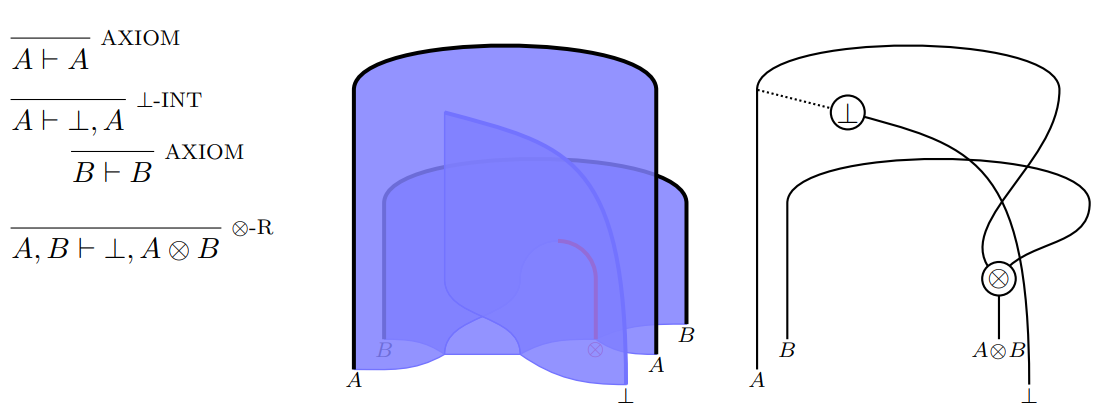
\includegraphics[width=130mm]{pictures/proof_net.png}
\caption{3D representation of proof nets \cite[Fig. 1]{dunn} }
\end{figure}




However, because proof nets are drawn on a 2-dimensional sheet of paper, the projection loses information: in particular the unit introduction and removal are degeneracies under the projection, making their connectivity  under the projection ambiguous. In \cite{ldc} the units are accounted for by using so-called ``thinning links,'' which we won't expose here as we shall not use it, and its combinatorial nature doesn't lead to a particularly elegant exposition.  This can be ignored in the case of monoidal categories, because they are inherently lower-dimensional objects; thus these problems with projections are assuaged. A direct construction of proof nets was later presented by \cite{wilson}, giving an inductive proof of MacLane's coherence theorem.  As well as giving a straightforward proof of the coherence theorem, this greatly simplified the exposition of proof nets in the monoidal case.

Proof nets have also been rediscovered in the compact closed case in the form of the scalable ZX-calculus \cite{szx} although they have not discovered the units and counits.  The scalable ZX-calculus has been since used extensively as a graphical calculus for quantum protocols where one seeks to index a register of wires, used prominently, for example in \cite{szxi,szxii}.  We will motivate this more in Section \ref{sec:cqm} when we introduce categorical quantum mechanics and the ZX-calculus.

On a separate note, linearly distributive categories have also been used to explore quantum causality \cite{sander} as well as to give toy models for infinite dimensional quantum processes  \cite{muc}.  Therefore, there is also motivation for understanding proof nets in the non-monoidal setting in the context of exploring quantum mechanics from a categorical perpsective, although it is not the focus of this thesis.


\subsection{Monoidal presentations}
In this section, we review how monoidal categories can be presented in terms of generators and equations. .





\begin{definition}
\label{def:monoidaltheory}

%A {\bf symmetric monoidal theory} is a triple $T=({\sf Ob},\Sigma ,E \)$. $\sf Ob$ is a set of {\em objects}. $\Sigma\in [{\sf Ob}]\times [{\sf Ob}]^{G}$ is a set of {\bf generators} $g$ with associated arities $(X,Y) \in [{\sf Ob}]\times [{\sf Ob}]$,  denoted $g:X\to Y$, where $[\_]$ is the finite list monad. Let $\Sigma'$ denote the set $\Sigma\sqcup\{c_X: [X,X]\to[X,X] | \forall X \in {\sf Ob} \}$, where the $c_X$ are regarded as the braiding maps.  Moreover, let $\Sigma^*$ denote the 
%$E \subseteq \{(f:X\to Y,g:X\to Y) \in \Sigma^2\}$

A {\bf monoidal theory} is a triple $T=({\sf Ob},\Sigma ,E )$ where: ${\sf Ob}$ is regarded as the set of generating objects; $\Sigma$, the set of generating morphisms with arities in $[{\sf Ob}]\times [{\sf Ob}]$, denoted $f:X\to Y$;  and $E$ the set of generating equations between parallel maps generated by $\Sigma$.

Every monoidal theory uniquely defines a strict monoidal category $\bar T$ given by quotienting the strict monoidal category freely generated by the objects in $\sf Ob$ and maps in $\Sigma$ modulo the equations in $E$.  Call such a monoidal category a {\bf multicoloured pro}, or merely a {\bf pro} when $|{\sf Ob}|=1$.  We will say that $T$ is a presentation of $\bar T$.
\end{definition}



 In practice, we won't explicitly regard a  monoidal theory as a triple; rather, we will present multicoloured pros by first drawing the string diagrams for all of the generators and then equations string diagrams for the equations. For example:

\begin{example}
Consider the monoidal theory for the prop $\m$ generated by a monoid on one object:


$$
\begin{tikzpicture}[yscale=-1]
	\begin{pgfonlayer}{nodelayer}
		\node [style=X] (10) at (8, 2) {};
		\node [style=none] (11) at (8.5, 2.75) {};
		\node [style=none] (12) at (7.5, 2.75) {};
		\node [style=none] (13) at (8, 1.25) {};
		\node [style=none] (14) at (8.5, 3.25) {};
		\node [style=X] (15) at (7.5, 2.75) {};
	\end{pgfonlayer}
	\begin{pgfonlayer}{edgelayer}
		\draw [in=-90, out=30] (10) to (11.center);
		\draw (13.center) to (10);
		\draw [in=-90, out=150] (10) to (12.center);
		\draw (11.center) to (14.center);
	\end{pgfonlayer}
\end{tikzpicture}
=
\begin{tikzpicture}[yscale=-1]
	\begin{pgfonlayer}{nodelayer}
		\node [style=none] (16) at (6.5, 1.25) {};
		\node [style=none] (17) at (6.5, 3.25) {};
	\end{pgfonlayer}
	\begin{pgfonlayer}{edgelayer}
		\draw (16.center) to (17.center);
	\end{pgfonlayer}
\end{tikzpicture}
=
\begin{tikzpicture}[yscale=-1]
	\begin{pgfonlayer}{nodelayer}
		\node [style=X] (4) at (5, 2) {};
		\node [style=none] (5) at (4.5, 2.75) {};
		\node [style=none] (6) at (5.5, 2.75) {};
		\node [style=none] (7) at (5, 1.25) {};
		\node [style=none] (8) at (4.5, 3.25) {};
		\node [style=X] (9) at (5.5, 2.75) {};
	\end{pgfonlayer}
	\begin{pgfonlayer}{edgelayer}
		\draw [in=-90, out=150] (4) to (5.center);
		\draw (7.center) to (4);
		\draw [in=-90, out=30] (4) to (6.center);
		\draw (5.center) to (8.center);
	\end{pgfonlayer}
\end{tikzpicture}
$$


This is a presentation for the pro, $\FinMon$, of finite ordinals and monotone maps.
\end{example}

\begin{definition}

A {\bf symmetric monoidal theory} $T$ consists of the same data as a monoidal theory except the equations are now defined by parallel maps generated by $\Sigma\sqcup C$, where  $C=\{c_X:[X,X]\to [X,X]|\forall X \in {\sf Ob}\}$ is the set of distinguished braiding maps.


The corresponding strict symmetric monoidal category $\bar T$ is given by quotienting the symmetric monoidal category freely generated by the objects $\sf Ob$ and morphisms $\Sigma$ by the equations in $E$.  These symmetric monoidal categories are called {\bf multicoloured props}, or merely {\bf props} when $|{\sf Ob}|=1$.
\end{definition}






\begin{example}
Consider the symmetric monoidal theory generated by a commutative monoid on one object:

$$
\begin{tikzpicture}[yscale=-1]
	\begin{pgfonlayer}{nodelayer}
		\node [style=X] (10) at (8, 2) {};
		\node [style=none] (11) at (8.5, 2.75) {};
		\node [style=none] (12) at (7.5, 2.75) {};
		\node [style=none] (13) at (8, 1.25) {};
		\node [style=none] (14) at (8.5, 3.25) {};
		\node [style=X] (15) at (7.5, 2.75) {};
	\end{pgfonlayer}
	\begin{pgfonlayer}{edgelayer}
		\draw [in=-90, out=30] (10) to (11.center);
		\draw (13.center) to (10);
		\draw [in=-90, out=150] (10) to (12.center);
		\draw (11.center) to (14.center);
	\end{pgfonlayer}
\end{tikzpicture}
=
\begin{tikzpicture}[yscale=-1]
	\begin{pgfonlayer}{nodelayer}
		\node [style=none] (16) at (6.5, 1.25) {};
		\node [style=none] (17) at (6.5, 3.25) {};
	\end{pgfonlayer}
	\begin{pgfonlayer}{edgelayer}
		\draw (16.center) to (17.center);
	\end{pgfonlayer}
\end{tikzpicture}
=
\begin{tikzpicture}[yscale=-1]
	\begin{pgfonlayer}{nodelayer}
		\node [style=X] (4) at (5, 2) {};
		\node [style=none] (5) at (4.5, 2.75) {};
		\node [style=none] (6) at (5.5, 2.75) {};
		\node [style=none] (7) at (5, 1.25) {};
		\node [style=none] (8) at (4.5, 3.25) {};
		\node [style=X] (9) at (5.5, 2.75) {};
	\end{pgfonlayer}
	\begin{pgfonlayer}{edgelayer}
		\draw [in=-90, out=150] (4) to (5.center);
		\draw (7.center) to (4);
		\draw [in=-90, out=30] (4) to (6.center);
		\draw (5.center) to (8.center);
	\end{pgfonlayer}
\end{tikzpicture}
\hspace*{1cm}
\begin{tikzpicture}[yscale=-1]
	\begin{pgfonlayer}{nodelayer}
		\node [style=X] (18) at (10, 2) {};
		\node [style=none] (19) at (10.5, 2.75) {};
		\node [style=none] (20) at (9.5, 2.75) {};
		\node [style=none] (21) at (10, 1.25) {};
		\node [style=none] (22) at (9.5, 3.75) {};
		\node [style=none] (23) at (10.5, 3.75) {};
	\end{pgfonlayer}
	\begin{pgfonlayer}{edgelayer}
		\draw [in=-90, out=30] (18) to (19.center);
		\draw (21.center) to (18);
		\draw [in=-90, out=150] (18) to (20.center);
		\draw [in=270, out=90] (19.center) to (22.center);
		\draw [in=270, out=90] (20.center) to (23.center);
	\end{pgfonlayer}
\end{tikzpicture}
=
\begin{tikzpicture}[yscale=-1]
	\begin{pgfonlayer}{nodelayer}
		\node [style=X] (24) at (12, 2) {};
		\node [style=none] (25) at (12.5, 2.75) {};
		\node [style=none] (26) at (11.5, 2.75) {};
		\node [style=none] (27) at (12, 1.25) {};
		\node [style=none] (28) at (12.5, 3.75) {};
		\node [style=none] (29) at (11.5, 3.75) {};
	\end{pgfonlayer}
	\begin{pgfonlayer}{edgelayer}
		\draw [in=-90, out=30] (24) to (25.center);
		\draw (27.center) to (24);
		\draw [in=-90, out=150] (24) to (26.center);
		\draw (25.center) to (28.center);
		\draw (26.center) to (29.center);
	\end{pgfonlayer}
\end{tikzpicture}
$$

This is a presentation for the prop of finite ordinals and functions.
This is a formal way to talk about the graph of a function between finite sets.

\end{example}

This elegant description of the symmetric monoidal category of finite sets motivates finding presentations for other well-known mathematical structures.

\begin{example}
Take semiring $S$.
Consider the prop generated by a commutative monoid and cocommutative comonoid:

$$
\begin{tikzpicture}[yscale=-1]
	\begin{pgfonlayer}{nodelayer}
		\node [style=X] (10) at (8, 2) {};
		\node [style=none] (11) at (8.5, 2.75) {};
		\node [style=none] (12) at (7.5, 2.75) {};
		\node [style=none] (13) at (8, 1.25) {};
		\node [style=none] (14) at (8.5, 3.25) {};
		\node [style=X] (15) at (7.5, 2.75) {};
	\end{pgfonlayer}
	\begin{pgfonlayer}{edgelayer}
		\draw [in=-90, out=30] (10) to (11.center);
		\draw (13.center) to (10);
		\draw [in=-90, out=150] (10) to (12.center);
		\draw (11.center) to (14.center);
	\end{pgfonlayer}
\end{tikzpicture}
=
\begin{tikzpicture}[yscale=-1]
	\begin{pgfonlayer}{nodelayer}
		\node [style=none] (16) at (6.5, 1.25) {};
		\node [style=none] (17) at (6.5, 3.25) {};
	\end{pgfonlayer}
	\begin{pgfonlayer}{edgelayer}
		\draw (16.center) to (17.center);
	\end{pgfonlayer}
\end{tikzpicture}
=
\begin{tikzpicture}[yscale=-1]
	\begin{pgfonlayer}{nodelayer}
		\node [style=X] (4) at (5, 2) {};
		\node [style=none] (5) at (4.5, 2.75) {};
		\node [style=none] (6) at (5.5, 2.75) {};
		\node [style=none] (7) at (5, 1.25) {};
		\node [style=none] (8) at (4.5, 3.25) {};
		\node [style=X] (9) at (5.5, 2.75) {};
	\end{pgfonlayer}
	\begin{pgfonlayer}{edgelayer}
		\draw [in=-90, out=150] (4) to (5.center);
		\draw (7.center) to (4);
		\draw [in=-90, out=30] (4) to (6.center);
		\draw (5.center) to (8.center);
	\end{pgfonlayer}
\end{tikzpicture},
\hspace*{.5cm}
\begin{tikzpicture}[yscale=-1]
	\begin{pgfonlayer}{nodelayer}
		\node [style=X] (18) at (10, 2) {};
		\node [style=none] (19) at (10.5, 2.75) {};
		\node [style=none] (20) at (9.5, 2.75) {};
		\node [style=none] (21) at (10, 1.25) {};
		\node [style=none] (22) at (9.5, 3.75) {};
		\node [style=none] (23) at (10.5, 3.75) {};
	\end{pgfonlayer}
	\begin{pgfonlayer}{edgelayer}
		\draw [in=-90, out=30] (18) to (19.center);
		\draw (21.center) to (18);
		\draw [in=-90, out=150] (18) to (20.center);
		\draw [in=270, out=90] (19.center) to (22.center);
		\draw [in=270, out=90] (20.center) to (23.center);
	\end{pgfonlayer}
\end{tikzpicture}
=
\begin{tikzpicture}[yscale=-1]
	\begin{pgfonlayer}{nodelayer}
		\node [style=X] (24) at (12, 2) {};
		\node [style=none] (25) at (12.5, 2.75) {};
		\node [style=none] (26) at (11.5, 2.75) {};
		\node [style=none] (27) at (12, 1.25) {};
		\node [style=none] (28) at (12.5, 3.75) {};
		\node [style=none] (29) at (11.5, 3.75) {};
	\end{pgfonlayer}
	\begin{pgfonlayer}{edgelayer}
		\draw [in=-90, out=30] (24) to (25.center);
		\draw (27.center) to (24);
		\draw [in=-90, out=150] (24) to (26.center);
		\draw (25.center) to (28.center);
		\draw (26.center) to (29.center);
	\end{pgfonlayer}
\end{tikzpicture},
\hspace*{.5cm}
\begin{tikzpicture}
	\begin{pgfonlayer}{nodelayer}
		\node [style=Z] (10) at (8, 2) {};
		\node [style=none] (11) at (8.5, 2.75) {};
		\node [style=none] (12) at (7.5, 2.75) {};
		\node [style=none] (13) at (8, 1.25) {};
		\node [style=none] (14) at (8.5, 3.25) {};
		\node [style=Z] (15) at (7.5, 2.75) {};
	\end{pgfonlayer}
	\begin{pgfonlayer}{edgelayer}
		\draw [in=-90, out=30] (10) to (11.center);
		\draw (13.center) to (10);
		\draw [in=-90, out=150] (10) to (12.center);
		\draw (11.center) to (14.center);
	\end{pgfonlayer}
\end{tikzpicture}
=
\begin{tikzpicture}
	\begin{pgfonlayer}{nodelayer}
		\node [style=none] (16) at (6.5, 1.25) {};
		\node [style=none] (17) at (6.5, 3.25) {};
	\end{pgfonlayer}
	\begin{pgfonlayer}{edgelayer}
		\draw (16.center) to (17.center);
	\end{pgfonlayer}
\end{tikzpicture}
=
\begin{tikzpicture}
	\begin{pgfonlayer}{nodelayer}
		\node [style=Z] (4) at (5, 2) {};
		\node [style=none] (5) at (4.5, 2.75) {};
		\node [style=none] (6) at (5.5, 2.75) {};
		\node [style=none] (7) at (5, 1.25) {};
		\node [style=none] (8) at (4.5, 3.25) {};
		\node [style=Z] (9) at (5.5, 2.75) {};
	\end{pgfonlayer}
	\begin{pgfonlayer}{edgelayer}
		\draw [in=-90, out=150] (4) to (5.center);
		\draw (7.center) to (4);
		\draw [in=-90, out=30] (4) to (6.center);
		\draw (5.center) to (8.center);
	\end{pgfonlayer}
\end{tikzpicture}\ ,
\hspace*{.5cm}
\begin{tikzpicture}
	\begin{pgfonlayer}{nodelayer}
		\node [style=Z] (18) at (10, 2) {};
		\node [style=none] (19) at (10.5, 2.75) {};
		\node [style=none] (20) at (9.5, 2.75) {};
		\node [style=none] (21) at (10, 1.25) {};
		\node [style=none] (22) at (9.5, 3.75) {};
		\node [style=none] (23) at (10.5, 3.75) {};
	\end{pgfonlayer}
	\begin{pgfonlayer}{edgelayer}
		\draw [in=-90, out=30] (18) to (19.center);
		\draw (21.center) to (18);
		\draw [in=-90, out=150] (18) to (20.center);
		\draw [in=270, out=90] (19.center) to (22.center);
		\draw [in=270, out=90] (20.center) to (23.center);
	\end{pgfonlayer}
\end{tikzpicture}
=
\begin{tikzpicture}
	\begin{pgfonlayer}{nodelayer}
		\node [style=Z] (24) at (12, 2) {};
		\node [style=none] (25) at (12.5, 2.75) {};
		\node [style=none] (26) at (11.5, 2.75) {};
		\node [style=none] (27) at (12, 1.25) {};
		\node [style=none] (28) at (12.5, 3.75) {};
		\node [style=none] (29) at (11.5, 3.75) {};
	\end{pgfonlayer}
	\begin{pgfonlayer}{edgelayer}
		\draw [in=-90, out=30] (24) to (25.center);
		\draw (27.center) to (24);
		\draw [in=-90, out=150] (24) to (26.center);
		\draw (25.center) to (28.center);
		\draw (26.center) to (29.center);
	\end{pgfonlayer}
\end{tikzpicture}
$$

Interacting to form a  bialgebra:
$$
\begin{tikzpicture}
	\begin{pgfonlayer}{nodelayer}
		\node [style=Z] (30) at (15, 2.25) {};
		\node [style=X] (31) at (15, 1.5) {};
		\node [style=none] (32) at (14.5, 0.75) {};
		\node [style=none] (33) at (15.5, 0.75) {};
		\node [style=none] (34) at (14.5, 3) {};
		\node [style=none] (35) at (15.5, 3) {};
	\end{pgfonlayer}
	\begin{pgfonlayer}{edgelayer}
		\draw (30) to (31);
		\draw [in=90, out=-150] (31) to (32.center);
		\draw [in=90, out=-30] (31) to (33.center);
		\draw [in=30, out=-90] (35.center) to (30);
		\draw [in=-90, out=150] (30) to (34.center);
	\end{pgfonlayer}
\end{tikzpicture}
=
\begin{tikzpicture}
	\begin{pgfonlayer}{nodelayer}
		\node [style=Z] (36) at (17, 1.5) {};
		\node [style=X] (37) at (17, 2.5) {};
		\node [style=Z] (42) at (17.75, 1.5) {};
		\node [style=X] (45) at (17.75, 2.5) {};
		\node [style=none] (46) at (17, 3.25) {};
		\node [style=none] (47) at (17.75, 3.25) {};
		\node [style=none] (48) at (17, 0.75) {};
		\node [style=none] (49) at (17.75, 0.75) {};
	\end{pgfonlayer}
	\begin{pgfonlayer}{edgelayer}
		\draw (42) to (37);
		\draw [bend right] (37) to (36);
		\draw (36) to (45);
		\draw [bend left] (45) to (42);
		\draw (37) to (46.center);
		\draw (47.center) to (45);
		\draw (49.center) to (42);
		\draw (36) to (48.center);
	\end{pgfonlayer}
\end{tikzpicture}\ ,
\hspace*{.5cm}
\begin{tikzpicture}
	\begin{pgfonlayer}{nodelayer}
		\node [style=Z] (50) at (19.25, 2.25) {};
		\node [style=X] (51) at (19.25, 1.5) {};
	\end{pgfonlayer}
	\begin{pgfonlayer}{edgelayer}
		\draw (50) to (51);
	\end{pgfonlayer}
\end{tikzpicture}
=
\begin{tikzpicture}
	\begin{pgfonlayer}{nodelayer}
		\node [style=none] (52) at (20, 2.25) {};
		\node [style=none] (53) at (20, 1.5) {};
		\node [style=none] (54) at (20.75, 1.5) {};
		\node [style=none] (55) at (20.75, 2.25) {};
	\end{pgfonlayer}
	\begin{pgfonlayer}{edgelayer}
		\draw [style=dashed] (52.center) to (53.center);
		\draw [style=dashed] (53.center) to (54.center);
		\draw [style=dashed] (54.center) to (55.center);
		\draw [style=dashed] (55.center) to (52.center);
	\end{pgfonlayer}
\end{tikzpicture}
$$
And generators for all elements $a,b \in k$ representing the structure of $k$ under convolution:

$$
\begin{tikzpicture}
	\begin{pgfonlayer}{nodelayer}
		\node [style=none] (0) at (0, 0.25) {};
		\node [style=none] (1) at (0, -2.25) {};
		\node [style=X] (2) at (0, -0.25) {};
		\node [style=Z] (3) at (0, -1.75) {};
		\node [style=none] (4) at (-0.5, -1) {};
		\node [style=none] (5) at (0.5, -1) {};
		\node [style=scalar,fill=white] (6) at (-0.5, -1) {$a$};
		\node [style=scalar,fill=white] (7) at (0.5, -1) {$b$};
	\end{pgfonlayer}
	\begin{pgfonlayer}{edgelayer}
		\draw (1.center) to (3);
		\draw (2) to (0.center);
		\draw [in=90, out=-30] (2) to (5.center);
		\draw [in=30, out=-90] (5.center) to (3);
		\draw [in=-90, out=150] (3) to (4.center);
		\draw [in=-150, out=90] (4.center) to (2);
	\end{pgfonlayer}
\end{tikzpicture}
=
\begin{tikzpicture}
	\begin{pgfonlayer}{nodelayer}
		\node [style=none] (0) at (0.5, 0.25) {};
		\node [style=none] (1) at (0.5, -2.25) {};
		\node [style=scalar] (2) at (0.5, -1) {$a+b$};
	\end{pgfonlayer}
	\begin{pgfonlayer}{edgelayer}
		\draw (2) to (0.center);
		\draw (1.center) to (2);
	\end{pgfonlayer}
\end{tikzpicture}\ ,
\hspace*{.5cm}
\begin{tikzpicture}
	\begin{pgfonlayer}{nodelayer}
		\node [style=none] (0) at (0.5, 0.25) {};
		\node [style=none] (1) at (0.5, -2.25) {};
		\node [style=scalar] (2) at (0.5, -0.5) {$b$};
		\node [style=scalar] (3) at (0.5, -1.5) {$a$};
	\end{pgfonlayer}
	\begin{pgfonlayer}{edgelayer}
		\draw (2) to (0.center);
		\draw (1.center) to (3);
		\draw (3) to (2);
	\end{pgfonlayer}
\end{tikzpicture}
=
\begin{tikzpicture}
	\begin{pgfonlayer}{nodelayer}
		\node [style=none] (0) at (0.5, 0.25) {};
		\node [style=none] (1) at (0.5, -2.25) {};
		\node [style=scalar] (2) at (0.5, -1) {$ab$};
	\end{pgfonlayer}
	\begin{pgfonlayer}{edgelayer}
		\draw (2) to (0.center);
		\draw (1.center) to (2);
	\end{pgfonlayer}
\end{tikzpicture}\ ,
\hspace*{.5cm}
\begin{tikzpicture}
	\begin{pgfonlayer}{nodelayer}
		\node [style=none] (0) at (0.5, 0.25) {};
		\node [style=none] (1) at (0.5, -1.25) {};
		\node [style=scalar] (2) at (0.5, -0.5) {$1$};
	\end{pgfonlayer}
	\begin{pgfonlayer}{edgelayer}
		\draw (2) to (0.center);
		\draw (1.center) to (2);
	\end{pgfonlayer}
\end{tikzpicture}
=
\begin{tikzpicture}
	\begin{pgfonlayer}{nodelayer}
		\node [style=none] (0) at (0.5, 0.25) {};
		\node [style=none] (1) at (0.5, -1.25) {};
	\end{pgfonlayer}
	\begin{pgfonlayer}{edgelayer}
		\draw (1.center) to (0.center);
	\end{pgfonlayer}
\end{tikzpicture}\ ,
\hspace*{.5cm}
\begin{tikzpicture}
	\begin{pgfonlayer}{nodelayer}
		\node [style=none] (0) at (0.5, 0.25) {};
		\node [style=none] (1) at (0.5, -1.25) {};
		\node [style=scalar] (2) at (0.5, -0.5) {$0$};
	\end{pgfonlayer}
	\begin{pgfonlayer}{edgelayer}
		\draw (2) to (0.center);
		\draw (1.center) to (2);
	\end{pgfonlayer}
\end{tikzpicture}
=
\begin{tikzpicture}
	\begin{pgfonlayer}{nodelayer}
		\node [style=none] (0) at (0.5, 0.25) {};
		\node [style=none] (1) at (0.5, -1.25) {};
		\node [style=X] (2) at (0.5, -0.25) {};
		\node [style=Z] (3) at (0.5, -0.75) {};
	\end{pgfonlayer}
	\begin{pgfonlayer}{edgelayer}
		\draw (2) to (0.center);
		\draw (3) to (1.center);
	\end{pgfonlayer}
\end{tikzpicture}
$$

Such that the commutative monoid and cocommutative comonoid are both natural with respect to the scalars:

$$
\begin{tikzpicture}
	\begin{pgfonlayer}{nodelayer}
		\node [style=Z] (12) at (2, 0) {};
		\node [style=none] (15) at (2.5, 0.75) {};
		\node [style=none] (17) at (2, -0.75) {};
		\node [style=none] (18) at (1.5, 0.75) {};
		\node [style=scalar,fill=white] (19) at (2, -0.75) {$a$};
		\node [style=none] (20) at (2, -1.5) {};
	\end{pgfonlayer}
	\begin{pgfonlayer}{edgelayer}
		\draw (17.center) to (12);
		\draw [in=-90, out=30] (12) to (15.center);
		\draw [in=150, out=-90] (18.center) to (12);
		\draw (20.center) to (17.center);
	\end{pgfonlayer}
\end{tikzpicture}
=
\begin{tikzpicture}
	\begin{pgfonlayer}{nodelayer}
		\node [style=Z] (21) at (3.75, -0.75) {};
		\node [style=none] (22) at (4.25, 0) {};
		\node [style=none] (23) at (3.75, -1.5) {};
		\node [style=none] (24) at (3.25, 0) {};
		\node [style=scalar,fill=white] (25) at (3.25, 0) {$a$};
		\node [style=scalar,fill=white] (27) at (4.25, 0) {$a$};
		\node [style=none] (28) at (3.25, 0.75) {};
		\node [style=none] (29) at (4.25, 0.75) {};
	\end{pgfonlayer}
	\begin{pgfonlayer}{edgelayer}
		\draw (23.center) to (21);
		\draw [in=-90, out=30] (21) to (22.center);
		\draw [in=150, out=-90] (24.center) to (21);
		\draw (28.center) to (25);
		\draw (29.center) to (27);
	\end{pgfonlayer}
\end{tikzpicture}
\ ,
\hspace*{.2cm}
\begin{tikzpicture}
	\begin{pgfonlayer}{nodelayer}
		\node [style=Z] (0) at (2, 0) {};
		\node [style=none] (2) at (2, -0.75) {};
		\node [style=scalar,fill=white] (4) at (2, -0.75) {$a$};
		\node [style=none] (5) at (2, -1.5) {};
	\end{pgfonlayer}
	\begin{pgfonlayer}{edgelayer}
		\draw (2.center) to (0);
		\draw (5.center) to (2.center);
	\end{pgfonlayer}
\end{tikzpicture}
=
\begin{tikzpicture}
	\begin{pgfonlayer}{nodelayer}
		\node [style=Z] (6) at (3.75, -0.75) {};
		\node [style=none] (8) at (3.75, -1.5) {};
	\end{pgfonlayer}
	\begin{pgfonlayer}{edgelayer}
		\draw (8.center) to (6);
	\end{pgfonlayer}
\end{tikzpicture}
\ ,
\hspace*{.2cm}
\begin{tikzpicture}
	\begin{pgfonlayer}{nodelayer}
		\node [style=X] (36) at (7.5, 0) {};
		\node [style=none] (37) at (8, -0.75) {};
		\node [style=none] (38) at (7.5, 0.75) {};
		\node [style=none] (39) at (7, -0.75) {};
		\node [style=scalar,fill=white] (40) at (7, -0.75) {$a$};
		\node [style=scalar,fill=white] (41) at (8, -0.75) {$a$};
		\node [style=none] (42) at (7, -1.5) {};
		\node [style=none] (43) at (8, -1.5) {};
	\end{pgfonlayer}
	\begin{pgfonlayer}{edgelayer}
		\draw (38.center) to (36);
		\draw [in=90, out=-30] (36) to (37.center);
		\draw [in=-150, out=90] (39.center) to (36);
		\draw (42.center) to (40);
		\draw (43.center) to (41);
	\end{pgfonlayer}
\end{tikzpicture}
=
\begin{tikzpicture}
	\begin{pgfonlayer}{nodelayer}
		\node [style=X] (30) at (5.75, -0.75) {};
		\node [style=none] (31) at (6.25, -1.5) {};
		\node [style=none] (32) at (5.75, 0) {};
		\node [style=none] (33) at (5.25, -1.5) {};
		\node [style=scalar,fill=white] (34) at (5.75, 0) {$a$};
		\node [style=none] (35) at (5.75, 0.75) {};
	\end{pgfonlayer}
	\begin{pgfonlayer}{edgelayer}
		\draw (32.center) to (30);
		\draw [in=90, out=-30] (30) to (31.center);
		\draw [in=-150, out=90] (33.center) to (30);
		\draw (35.center) to (32.center);
	\end{pgfonlayer}
\end{tikzpicture}
\ ,
\hspace*{.2cm}
\begin{tikzpicture}
	\begin{pgfonlayer}{nodelayer}
		\node [style=X] (15) at (7.5, 0) {};
		\node [style=none] (17) at (7.5, 0.75) {};
	\end{pgfonlayer}
	\begin{pgfonlayer}{edgelayer}
		\draw (17.center) to (15);
	\end{pgfonlayer}
\end{tikzpicture}
=
\begin{tikzpicture}
	\begin{pgfonlayer}{nodelayer}
		\node [style=X] (9) at (5.75, -0.75) {};
		\node [style=none] (11) at (5.75, 0) {};
		\node [style=scalar,fill=white] (13) at (5.75, 0) {$a$};
		\node [style=none] (14) at (5.75, 0.75) {};
	\end{pgfonlayer}
	\begin{pgfonlayer}{edgelayer}
		\draw (11.center) to (9);
		\draw (14.center) to (11.center);
	\end{pgfonlayer}
\end{tikzpicture}
$$



This monoidal theory is equivalent to the prop of matrices over $S$ $\Mat(S)$ under the direct sum.
\end{example}


One can glue monoidal theories together:


\begin{lemma}
Take three symmetric monoidal theories

$$T_0=({\sf Ob}_0,\Sigma_0 ,E_0 ), \ T_1=({\sf Ob}_1,\Sigma_1 ,E_1 ), \ T_2=({\sf Ob}_2,\Sigma_2 ,E_2 )$$

such that $\bar{T_0}$ is a sub-pro(p) of both $\bar{T_1}$ and $\bar{T_2}$ and $\Sigma_0 \subseteq \Sigma_1$ and $\Sigma_2$.
Then the pushout of the diagram $\bar{T_1} \leftarrow \bar{T_0} \rightarrow \bar{T_2}$  in the category of strict (symmetric) monoidal categories is presented by the (symmetric) monoidal theory:

$$
( {\sf Ob}_1 +_{{\sf Ob}_0} {\sf Ob}_2, \Sigma_0+\Sigma_1, E_1 \cup E_2 \cup E_3 )
$$

\end{lemma}

We will use this presentation extensively throughout the thesis.  We will also use the following:

\begin{example}
Consider the symmetric monoidal theory generated by a commutative monoid in addition to this new generator and equation:

$$
\begin{tikzpicture}
	\begin{pgfonlayer}{nodelayer}
		\node [style=none] (0) at (0.5, 0.5) {};
		\node [style=X] (2) at (0.5, -0.25) {$1$};
		\node [style=Z] (3) at (0.5, 0.5) {};
		\node [style=none] (4) at (0, 1.25) {};
		\node [style=none] (5) at (1, 1.25) {};
	\end{pgfonlayer}
	\begin{pgfonlayer}{edgelayer}
		\draw (2) to (0.center);
		\draw [in=270, out=150] (3) to (4.center);
		\draw [in=270, out=30] (3) to (5.center);
	\end{pgfonlayer}
\end{tikzpicture}
=
\begin{tikzpicture}
	\begin{pgfonlayer}{nodelayer}
		\node [style=X] (7) at (2, -0.25) {$1$};
		\node [style=none] (9) at (2, 1.25) {};
		\node [style=none] (10) at (3, 1.25) {};
		\node [style=X] (11) at (3, -0.25) {$1$};
	\end{pgfonlayer}
	\begin{pgfonlayer}{edgelayer}
		\draw (7) to (9.center);
		\draw (11) to (10.center);
	\end{pgfonlayer}
\end{tikzpicture},
\hspace*{.5cm}
\begin{tikzpicture}
	\begin{pgfonlayer}{nodelayer}
		\node [style=none] (0) at (0.5, 0.5) {};
		\node [style=X] (2) at (0.5, -0.25) {$1$};
		\node [style=Z] (3) at (0.5, 0.5) {};
	\end{pgfonlayer}
	\begin{pgfonlayer}{edgelayer}
		\draw (2) to (0.center);
	\end{pgfonlayer}
\end{tikzpicture}
=
\begin{tikzpicture}
	\begin{pgfonlayer}{nodelayer}
		\node [style=none] (12) at (0, -0.25) {};
		\node [style=none] (13) at (0, 0.5) {};
		\node [style=none] (14) at (-0.75, 0.5) {};
		\node [style=none] (15) at (-0.75, -0.25) {};
	\end{pgfonlayer}
	\begin{pgfonlayer}{edgelayer}
		\draw [style=dashed] (12.center) to (13.center);
		\draw [style=dashed] (13.center) to (14.center);
		\draw [style=dashed] (14.center) to (15.center);
		\draw [style=dashed] (15.center) to (12.center);
	\end{pgfonlayer}
\end{tikzpicture}
$$


We see that $\FSet^\op$ embeds in this prop as well as in the prop $\Mat(S)$ for some semiring $S$.  The pushout of this diagram is presented by adding this generator and equations to the presentation of $\Mat(S)$.  This is a presentation for the prop of affine matrices over $S$.
\end{example}




There is another  more elegant way to compose presentations of monoidal and symmetric monoidal categories (via distributive law).  We will introduce this notion slightly later, because it requires a considerable amount of mathematical machinery to expose.

%Notice that the coproduct is a special case of the pushout.

\subsection{Dagger-monoidal categories}
In this thesis, we will usually work with monoidal categories with extra structure called the dagger which allows one in some sense to``run maps in reverse:''


\begin{definition}
A {\bf \dag-category} ({\em read dagger-category}) is a category $\X$ equipped with a functor ${(\_)}^\dag:\X^\op\to\X$ (the dagger) which is:

\begin{description}
\item[\ \ Identity on objects:] so that for all objects $X$ of $\X$, $X^\dag = X$.
\item[\ \ Involutive:] so that for all maps $f$ of $\X$, $(f^\dag)^\dag = f$.
\end{description}

A map $f$ in a dagger category is an:

\begin{description}
\item[\ \ Isometry] when $f^\dag; f = 1$.
\item[\ \ Coisometry] when $f; f^\dag = 1$.
\item[\ \ Unitary] when $f^\dag = f^{-1}$.
\item[\ \ Projector] such that $f;f=f$ and $f^\dag=f$ (also known as a $\dag$-idempotent).
\end{description}

\end{definition}


\begin{example}
 $\Mat_\C$ is a \dag-category with respect to both the transpose and the complex conjugate transpose.
\end{example}

\begin{example}

The category $\Hilb$ of complex Hilbert spaces and bounded linear maps is a dagger category with respect to the Hermetian adjoint.  The Hermetian adjoint of a map $A$ is the unique map $A^\dag$ satifying the following equation:
$$
\langle x;A|y\rangle = \langle x | A^\dag; y \rangle
$$


Let $\FHilb$ denote the full subcategory of finite dimensional Hilbert spaces of $\Hilb$.  This is also a $\dag$-category.
\end{example}

\begin{lemma}
There is an equivalence of categories $\FHilb \cong \Mat_\C$ preserving and reflecting the dagger structure.
The Hermetian conjugate of finite dimensional Hilbert spaces corresponds to the complex conjugate transpose along the equivalence $\Mat_\C \cong \FHilb$.
\end{lemma}



There is a natural way to combined monoidal and dagger structure:

\begin{definition}
A {\bf  (strict) \dag-(symmetric) monoidal category} is a (strict) (symmetric) monoidal category equipped with a strict (symmetric) dagger functor with respect to which all the components of the  coherence isomorphisms of the (symmetric) monoidal structure are unitary.
\end{definition}



\begin{example}
The dagger category and symmetric monoidal structures of $\FHilb$, $\Hilb$ and $\Mat_\C$ are all compatible making them \dag-symmetric monoidal categories.
\end{example}


We capture more of monoidal category theory within the framework of dagger categories:

\begin{definition}
A {(strict) \dag-compact closed category} is a (strict) compact closed category which is (strict) \dag-symmetric monoidal and for all objects $\X$:

$$
\xymatrix{
I \ar[r]^{\epsilon_X^\dag} \ar[dr]_{\eta_X}   &  X\otimes X^* \ar[d]^{c_{X,X^*}}\\
                                                                        &  X^* \otimes X 
}
$$
\end{definition}

\begin{example}
$\Mat_\C$ is a strict \dag-compact closed category with respect to both the transpose and the complex conjugate transpose.  
$\FHilb$ is \dag-compact closed with respect to the  Hermetian adjoint.

\end{example}

Note that $\Hilb$ is not a $\dag$-compact closed category anymore!




\subsection{Spans and relations in computation}

Categories are defined in a manner which distinguishes the inputs and outputs of morphisms.  \dag-categories are one approach to moving beyond this bias; however, they are evil in the sense are the \dag-structure is not always preserved/reflected by categorical equivalence: the theory of \dag-categories does not play well with the theory of ordinary categories.  

Spans and relations provide a categorically well-behaved, flexible setting with which to interpret processes without elevating inputs over outputs.
If functions are produce unique outputs from inputs, spans and relations nondeterministicaly associate several inputs with several outputs.  To introduce these mathematical constructions, we first need to recall some basic facts about limits: 



\begin{definition}
The {\bf product} of two objects $X$ and $Y$ (if it exists) in some category, is an object $X\times Y$ equipped with maps $\pi_0:X\times Y\to X $ and $\pi_1:X\times Y \to Y$ called the {\bf projections},  such that for any object $A$ and diagram  $X \xleftarrow{f} A \xrightarrow{g} Y$ there exists a unique map $\langle  f, g \rangle :A \to X\times Y$ called {\bf the pairing map} making the following diagram commute:


$$
\xymatrix{
    &
    & A \ar[lld]_f \ar[rrd]^g \ar@{-->}[d]^{\langle f,g\rangle}
    &
    &
  \\X 
    &
    & X\times Y \ar[ll]^{\pi_0} \ar[rr]_{\pi_1}
    &
    & Y
}
$$ 

Given two maps $f:W\to X$ and $G:Y\to Z$, their product is defined to be the universal map $f\times g:W\times Y \to X\times Z$: 

$$
\xymatrix{
    W \ar[d]_f
    &
    & W\times Y \ar@{-->}[d]^{f\times g} \ar[ll]_{\pi_0} \ar[rr]^{\pi_1}
    &
    & Y \ar[d]^g
  \\X
    &
    & Y\times Z  \ar[ll]_{\pi^0} \ar[rr]_{\pi_1}
    &
    &Z
}
$$


A terminal object in a category (if it exists) is an object $1$ equipped with a unique map $1:X\to 1$ for every object $1$ called the {\bf discard map}.



A category is  {\bf Cartesian } when it has all finite products and a terminal object. In a Cartesian category, the discard maps and {\bf diagonals} $\langle 1, 1 \rangle$ yield a natural family of commutative monoids.


The products/projections/pairing maps/terminal objects/cartesian categories/diagonal maps in $\X$ are respectively {\bf coproducts}/{\bf injections}/{\bf copairing maps}/{\bf initial objects}/{\bf cocartesian categories}/{\bf codiagonal maps} in $\X^\op$.

\end{definition}

The basic idea is that Cartesian categories axiomatize copying, and coCartesian categories axiomatize comparison.

\begin{lemma}
A category is cartesian iff it is equipped with a natural supply of cocommutative comonoids compatible with the tensor product:


$$
\begin{tikzpicture}
	\begin{pgfonlayer}{nodelayer}
		\node [style=none] (0) at (0, 2.5) {};
		\node [style=none] (1) at (1, 2.5) {};
		\node [style=Z] (2) at (0.5, 1.5) {};
		\node [style=none] (3) at (0.5, 0.5) {};
	\end{pgfonlayer}
	\begin{pgfonlayer}{edgelayer}
		\draw [style=simple] (3.center) to (2);
		\draw [style=simple, in=-90, out=117] (2) to (0.center);
		\draw [style=simple, in=63, out=-90] (1.center) to (2);
	\end{pgfonlayer}
\end{tikzpicture}
=
\begin{tikzpicture}
	\begin{pgfonlayer}{nodelayer}
		\node [style=Z] (0) at (0, 2.5) {};
		\node [style=Z] (1) at (1, 2.5) {};
		\node [style=none] (2) at (0.5, 1.5) {};
		\node [style=none] (3) at (0.5, 0.5) {};
		\node [style=none] (4) at (0, 3.5) {};
		\node [style=none] (5) at (1, 3.5) {};
		\node [style=none] (6) at (0, 4.5) {};
		\node [style=none] (7) at (1, 4.5) {};
		\node [style=otimes] (8) at (0.5, 1.5) {};
		\node [style=otimes] (9) at (1, 3.5) {};
		\node [style=otimes] (10) at (0, 3.5) {};
	\end{pgfonlayer}
	\begin{pgfonlayer}{edgelayer}
		\draw [style=simple] (3.center) to (2.center);
		\draw [style=simple, in=-90, out=135] (2.center) to (0);
		\draw [style=simple] (0) to (5.center);
		\draw [style=simple, in=120, out=-120, looseness=1.25] (4.center) to (0);
		\draw [style=simple, in=-60, out=60, looseness=1.25] (1) to (5.center);
		\draw [style=simple] (1) to (4.center);
		\draw [style=simple, in=45, out=-90] (1) to (2.center);
		\draw [style=simple] (4.center) to (6.center);
		\draw [style=simple] (5.center) to (7.center);
	\end{pgfonlayer}
\end{tikzpicture}
\ ,
\hspace*{.2cm}
\begin{tikzpicture}
	\begin{pgfonlayer}{nodelayer}
		\node [style=Z] (2) at (1, 1.5) {};
		\node [style=none] (3) at (1, 0.5) {};
	\end{pgfonlayer}
	\begin{pgfonlayer}{edgelayer}
		\draw [style=simple] (3.center) to (2);
	\end{pgfonlayer}
\end{tikzpicture}
=
\begin{tikzpicture}
	\begin{pgfonlayer}{nodelayer}
		\node [style=Z] (4) at (2.5, 2.5) {};
		\node [style=Z] (5) at (3.5, 2.5) {};
		\node [style=none] (6) at (3, 1.5) {};
		\node [style=none] (7) at (3, 0.5) {};
		\node [style=otimes] (12) at (3, 1.5) {};
	\end{pgfonlayer}
	\begin{pgfonlayer}{edgelayer}
		\draw [style=simple] (7.center) to (6.center);
		\draw [style=simple, in=-90, out=135] (6.center) to (4);
		\draw [style=simple, in=45, out=-90] (5) to (6.center);
	\end{pgfonlayer}
\end{tikzpicture}$$
$$
\begin{tikzpicture}[xscale=-1]
	\begin{pgfonlayer}{nodelayer}
		\node [style=Z] (0) at (5.75, -0.75) {};
		\node [style=none] (1) at (6.25, 0) {};
		\node [style=none] (2) at (5.75, -1.5) {};
		\node [style=none] (3) at (5.25, 0) {};
		\node [style=none] (5) at (5.25, 0.75) {};
		\node [style=Z] (6) at (6.25, 0) {};
	\end{pgfonlayer}
	\begin{pgfonlayer}{edgelayer}
		\draw (2.center) to (0);
		\draw [in=-90, out=30] (0) to (1.center);
		\draw [in=150, out=-90] (3.center) to (0);
		\draw [in=270, out=90] (3.center) to (5.center);
	\end{pgfonlayer}
\end{tikzpicture}
=
\begin{tikzpicture}
	\begin{pgfonlayer}{nodelayer}
		\node [style=none] (9) at (7.25, -1.5) {};
		\node [style=none] (11) at (7.25, 0.75) {};
	\end{pgfonlayer}
	\begin{pgfonlayer}{edgelayer}
		\draw (11.center) to (9.center);
	\end{pgfonlayer}
\end{tikzpicture}
=
\begin{tikzpicture}
	\begin{pgfonlayer}{nodelayer}
		\node [style=Z] (0) at (5.75, -0.75) {};
		\node [style=none] (1) at (6.25, 0) {};
		\node [style=none] (2) at (5.75, -1.5) {};
		\node [style=none] (3) at (5.25, 0) {};
		\node [style=none] (5) at (5.25, 0.75) {};
		\node [style=Z] (6) at (6.25, 0) {};
	\end{pgfonlayer}
	\begin{pgfonlayer}{edgelayer}
		\draw (2.center) to (0);
		\draw [in=-90, out=30] (0) to (1.center);
		\draw [in=150, out=-90] (3.center) to (0);
		\draw [in=270, out=90] (3.center) to (5.center);
	\end{pgfonlayer}
\end{tikzpicture}
\ ,
\hspace*{.2cm}
\begin{tikzpicture}
	\begin{pgfonlayer}{nodelayer}
		\node [style=Z] (21) at (3.75, -0.75) {};
		\node [style=none] (22) at (4.25, 0) {};
		\node [style=none] (23) at (3.75, -1.5) {};
		\node [style=none] (24) at (3.25, 0) {};
		\node [style=none] (28) at (3.25, 0.75) {};
		\node [style=none] (29) at (4.25, 0.75) {};
	\end{pgfonlayer}
	\begin{pgfonlayer}{edgelayer}
		\draw (23.center) to (21);
		\draw [in=-90, out=30] (21) to (22.center);
		\draw [in=150, out=-90] (24.center) to (21);
		\draw [in=270, out=90] (22.center) to (28.center);
		\draw [in=270, out=90] (24.center) to (29.center);
	\end{pgfonlayer}
\end{tikzpicture}
=
\begin{tikzpicture}
	\begin{pgfonlayer}{nodelayer}
		\node [style=Z] (30) at (5.75, -0.75) {};
		\node [style=none] (31) at (6.25, 0) {};
		\node [style=none] (32) at (5.75, -1.5) {};
		\node [style=none] (33) at (5.25, 0) {};
		\node [style=none] (34) at (6.25, 0.75) {};
		\node [style=none] (35) at (5.25, 0.75) {};
	\end{pgfonlayer}
	\begin{pgfonlayer}{edgelayer}
		\draw (32.center) to (30);
		\draw [in=-90, out=30] (30) to (31.center);
		\draw [in=150, out=-90] (33.center) to (30);
		\draw [in=270, out=90] (31.center) to (34.center);
		\draw [in=270, out=90] (33.center) to (35.center);
	\end{pgfonlayer}
\end{tikzpicture}\ ,
\hspace*{.2cm}
\begin{tikzpicture}
	\begin{pgfonlayer}{nodelayer}
		\node [style=Z] (12) at (2, 0) {};
		\node [style=none] (15) at (2.5, 0.75) {};
		\node [style=none] (17) at (2, -0.75) {};
		\node [style=none] (18) at (1.5, 0.75) {};
		\node [style=map] (19) at (2, -0.75) {$f$};
		\node [style=none] (20) at (2, -1.5) {};
	\end{pgfonlayer}
	\begin{pgfonlayer}{edgelayer}
		\draw (17.center) to (12);
		\draw [in=-90, out=30] (12) to (15.center);
		\draw [in=150, out=-90] (18.center) to (12);
		\draw (20.center) to (17.center);
	\end{pgfonlayer}
\end{tikzpicture}
=
\begin{tikzpicture}
	\begin{pgfonlayer}{nodelayer}
		\node [style=Z] (21) at (3.75, -0.75) {};
		\node [style=none] (22) at (4.25, 0) {};
		\node [style=none] (23) at (3.75, -1.5) {};
		\node [style=none] (24) at (3.25, 0) {};
		\node [style=map] (25) at (3.25, 0) {$f$};
		\node [style=map] (27) at (4.25, 0) {$f$};
		\node [style=none] (28) at (3.25, 0.75) {};
		\node [style=none] (29) at (4.25, 0.75) {};
	\end{pgfonlayer}
	\begin{pgfonlayer}{edgelayer}
		\draw (23.center) to (21);
		\draw [in=-90, out=30] (21) to (22.center);
		\draw [in=150, out=-90] (24.center) to (21);
		\draw (28.center) to (25);
		\draw (29.center) to (27);
	\end{pgfonlayer}
\end{tikzpicture} \ ,
\hspace*{.2cm}
\begin{tikzpicture}
	\begin{pgfonlayer}{nodelayer}
		\node [style=Z] (0) at (2, 0) {};
		\node [style=none] (2) at (2, -0.75) {};
		\node [style=map] (4) at (2, -0.75) {$f$};
		\node [style=none] (5) at (2, -1.5) {};
	\end{pgfonlayer}
	\begin{pgfonlayer}{edgelayer}
		\draw (2.center) to (0);
		\draw (5.center) to (2.center);
	\end{pgfonlayer}
\end{tikzpicture}
=
\begin{tikzpicture}
	\begin{pgfonlayer}{nodelayer}
		\node [style=Z] (6) at (3.75, -0.75) {};
		\node [style=none] (8) at (3.75, -1.5) {};
	\end{pgfonlayer}
	\begin{pgfonlayer}{edgelayer}
		\draw (8.center) to (6);
	\end{pgfonlayer}
\end{tikzpicture}
$$
\end{lemma}

The following Lemma justfies thinking of our running  examples of (finite) sets under the Cartesian product and matrices, vector spaces, hilbert spaces under the direct sum as symmetric monoidal categories.  Similarly, for (finite) sets as a symmetric monoidal categories under the coproduct.

\begin{lemma}
(Co)cartesian categories are symmetric monoidal with respect to the (co)product as the tensor and the initial/terminal object as the unit.
\end{lemma}




As we alluded to in the introduction of this subsection, the Cartesian notion of copying is biases inputs over outputs; however, this is fundamentally incompatible with dagger structure.  We are interested in a more permissive, symmetric notion of copying. The following notion allows us to develop such a structure:


\begin{definition}
The {\bf pullback} of a diagram  $X \xrightarrow{f} A \xleftarrow{g} Y$ (if it exists) is an object $X\ {}_f \times_{g} Y$ called and maps $\pi_0:X\ {}_f \times_{g} Y\to X$ and  $\pi_1:X\ {}_f \times_{g} Y\to Y$ called {\bf the  projections}, such that for any diagram $X \xleftarrow{p_0} P \xrightarrow{p_1} Y$ making the the following diagram commute:

$$
\xymatrix{
    &
    & B   \ar[dll]_{p_0} \ar[drr]^{p^1}
    &
    &
  \\X \ar[drr]_f 
    &
    & 
    &
    & Y  \ar[dll]^{g}
  \\
    &
    & A
    &
    & 
}
$$

There exists a unique map $u: P\to X\ {}_f\times_g Y $ called the {\bf pairing map} making the following diagram commute:

$$
\xymatrix{
    &
    & P \ar@/_/[ddll]_{p_0}  \ar@/^/[ddrr]^{p_1} \ar@{-->}[d]^{u}
    &
    &
  \\
    &
    & X\ {}_f \times_{g} Y  \ar[dll]_{\pi_0} \ar[drr]^{\pi_1}
    &
    &
  \\X \ar[drr]_f 
    &
    & 
    &
    & Y \ar[dll]^g 
  \\
    &
    & A
    &
    & 
}
$$

A category is {\bf finitely complete} if it has a terminal object and all pullbacks exist. Notice that product $X\times Y$ is the pullback of the diagram $X \rightarrow 1 \leftarrow Y$.
\end{definition}

\begin{example} 
In Sets the pullback of a cospan $X \xrightarrow{f} A \xleftarrow{g} Y$ is (up to unique isomorphism) the set $\{(x,y) \in X\times Y : f(x) = g(y)\}$.


The concrete pullback of matrices is essentially the same, with the product the direct sum.
\end{example}

Spans form a 2-category under pullback:
\begin{definition}
Given a finitely complete category $\X$, the 2-category of spans $\Span(\X)$ has:

\begin{description}
\item[\ \ 0-cells:] Objects of $\X$.
\item[\ \ 1-cells:] 1-cells $(A,f,g):X\to Y$ are spans in $\X$ from $A$:

$$
\xymatrix{
    & A \ar[dl]_{f} \ar[dr]^{g}
    &
  \\X 
    &
    & Y
}
$$

Composition is given by the span induced by pullback:
$$
\xymatrix{
    & A\ar[dl]_{f} \ar[dr]^{g}
    &
  \\X 
    &
    & Y
}\ ;\
\xymatrix{
    & B\ar[dl]_{h} \ar[dr]^{k}
    &
  \\Y 
    &
    & Z
}
:=
\xymatrix{
    &
    & A {}_g\times_k B \ar[dl]_{\pi_0} \ar[dr]^{\pi_1}
    &
    &
  \\
    & A \ar[dl]_{f} \ar[dr]^{g}
    &
    & B \ar[dl]_{h} \ar[dr]^{k}
    &
  \\X
    &
    & Y
    &
    & Z
}
$$

The identity on $X$ is given by the span:

$$
\xymatrix{
    & X \ar@{=}[dl] \ar@{=}[dr] 
    &
  \\X 
    &
    & X
}
$$
%ooPoo
%oAoBo
%XoYoZ

\item[\ \ 2-cells:] A 2-cell $\phi:(A,f,g)\Rightarrow (B,h,k)$ between parallel spans is a map $f:A\to B$ in $\X$ such that the following diagram commute

$$
\xymatrix{
    & A \ar[dl]_{f} \ar[dr]^{g} \ar[dd]^{\phi}
    &
  \\X 
    &
    & Y
  \\
    & B \ar[ul]^{h} \ar[ur]_{k}
    &
}
$$

The composition and identity of  2-cells is given by the compostition and identity in $\X$.
\end{description}

Note that composition of 1-cells is not strict, so that the associativity and unitality of composition hold up to coherent isomorphism.  The coherence isomorphisms are the natural 2-cells induced by the universal property of the pullback.


The 1-category of spans of $\X$, $\Span^\sim(\X)$, has maps being equivalence classes of isomorphic spans. 
\end{definition}


TODO  Frobenius algebra structure


Categories of spans give mathematical semantics for nondeterminstic processes where inputs are associated to possible outputs with multiplicity.  The Frobenius algebra is interpreted as a nondeterministic branching which allows for inputs and outputs to be related to each other in multiple ways.
A 2-cell between two processes thus describes a method to transform one process into another in a way that preserves the relationships between inputs and outputs.
Notice that one can have many parallel unequal 2-cells.


\begin{lemma}
TODO MORE Spans of finite sets are matrices over the natural numbers
\end{lemma}

In a sense, one can interpret the element of a matrix at coordinates $i,j$ as the number of possible ways to transition from index $j$ to index $i$.


  We seek moreover, to quotient by multiplicity, to obtain a semantics for merely possibilistic processes.  To do so, we need more assumptions about the category with which we seek to work internal to.


\begin{definition}
The {\bf equalizer}, of two parallel maps $f,g:X\to Y$, if it exists, is an object $E_{f,g}$ equipped with a map $m:E_{f,g}\to X$ such that for all objects $F$ and maps $h:F\to E_{f,g}$, there exists a unique map $u:F\to A$ such that the following diagram commutes:

$$
\xymatrix{
    F \ar@{-->}[dr]^{u} \ar[d]_h
  \\ E_{f,g} \ar[r]_e
    & X \ar@<-.5ex>[r]_g \ar@<.5ex>[r]^f
    & Y
}
$$

The maps $e$ arising from equalizers are monomorphisms.  Monomorphisms arising this way are called {\bf regular monomorphisms}.


The dual notion to an equalizer is a {\bf coequalizer}, and the epimorphisms arizing in this way are called {\bf regular epimorphisms}.
\end{definition}



\begin{lemma}
Epi mono factorization TODO
\end{lemma}


\begin{example}
Sets and matrices both have equalizers.

In sets, the equalizer of two functions $g,f:X\to Y$ is (up to unique isomorphism) the set $\{x \in X:f(x)=g(x)\} \subseteq X$.

The coequalizer is the quotient $Y/\sim$   of the set $Y$ by the equivalence relation $f(x)\sim f(y)$.

The situation is essentially the same for matrices.
\end{example}


\begin{definition}
A {\bf regular category} is a finitely complete category where moreover:

\begin{itemize}
\item For any map $f:X\to Y$, the pullback of $f$ along itself $\xymatrix{X\ {}_f \times_f X  \ar@<-.5ex>[r]_{\ \ \ \ \pi_0;f} \ar@<.5ex>[r]^{\ \ \ \ \pi_0;f} & Y}$ admits a coequalizer.

\item Pullbacks of arbitrary maps along regular epimorphisms are regular epimorphisms.
\end{itemize}

\end{definition}


\begin{example}
Sets, finite sets and matrices over a field are all regular categories.
\end{example}


\begin{definition}
Given a regular category $\X$, define the 2-category of {\bf relations} internal to $\X$, $\Rel(\X)$ has:

\begin{description}
\item[0-cells:] Objects of $\X$.
\item[1-cells:] 1-cells $(A,f,g):X\to Y$ are jointly monic spans in $\X$ from $A$:


$$
\xymatrix{
    & A \ar[dl]_{f} \ar[dr]^{g}
    &
  \\X 
    &
    & Y
}
$$
This span being {\bf jointly monic} means that for any object $B$ and morphisms $h,k:B\to A$ if $h;f=k;f$ and $h;g=k;g$, then $h=k$.

To compose jointly monic spans $(A,f,g):X\to Y$ and $(B,h,k):Y\to Z$,  first compute the pullback
$$
\xymatrix{
    &
    & A\ {}_g\times_k B \ar[dl]_{\pi_0} \ar[dr]^{\pi_1}
    &
    &
  \\
    & A \ar[dl]_{f} \ar[dr]^{g}
    &
    & B \ar[dl]_{h} \ar[dr]^{k}
    &
  \\X
    &
    & Y
    &
    & Z
}
$$

Composing with the pairing map we get a map $\langle \pi_0;f,\pi_1;k\rangle :A {}_g\times_k B \to X\times Z$.
Because $\X$ is a regular category, there is a factorization 

$$
\xymatrix{
  A\ {}_g\times_k B \ar[dr]^{\langle \pi_0;f,\pi_1;k\rangle}  \ar@{->>}[d]
  \\ E \ar@{>->}[r]_{e}
    &  X\times Z
}
$$

Which induces a jointly monic span, which we take to be the composite:

$$
\xymatrix{
    & A \ar[dl]_{f} \ar[dr]_{g}
    &
  \\X 
    &
    & Y
};
\xymatrix{
    & B \ar[dl]_{f} \ar[dr]_{g}
    &
  \\Y 
    &
    & Z
}
:=
\xymatrix{
    & E \ar[dl]_{e;\pi_0} \ar[dr]^{e;\pi_1}
    &
  \\X 
    &
    & Y
}
$$

The identity for composition is the same as for spans.

\item[2-cells:] The 2-cells and their composition and identity is the same as for spans.

\end{description}

\end{definition}

Relations have the special propert, unlike spans, that they are poset-enriched; that is to say, either there exists a single 2-cell between 1-cells or there doesn't. This makes things much simpler than the spans picture, because one never has to deal with coherence equations.  This also justifies the interpretation of possibilistic processes in this setting: possibility amounts to the mere existence of a 2-cell.  Any two ways to arrive at the same result must be the same.


We give a concrete description of the canonical example of internal relations.


\begin{example}
$\Rel=\Rel(\Set)$ has:

\begin{description}
\item[0-cells:] Natural numbers.

\item[1-cells:] A relation from $n\to m$ is a a subset $X \times Y$.

The composition of relations $R \subseteq X \times Y$  and $S \subseteq Y \times Z$ is given by:
$$
R;S := \{  (x,z) \in X\times Z: \exists y \in Y, (x,y) \in R \wedge (y,z) \in S \} \subseteq X\times Z
$$ 

\item[2-cells:] 
A 2-cell $R\Rightarrow S$ is a subset $R\subseteq S$.
\end{description}

Finite relations $\FRel=\Rel(\FSet)$, linear relations $\LinRel=\Rel(\Mat_k)$ are defined in the same way.
\end{example}



Relations of finite sets have a familiar presentation:

\begin{lemma}
Relations of finite sets is isomorphic to matrices over the boolean semiring.
\end{lemma}



Notice how spans of finite sets are matrices over the natural numbers; whereas relations are matrices over the Boolean semiring.  This gives some concrete evidence for how the quotient going from spans to relations forgets about multiplicity.


In the dual picture, corelations can be interpreted as the algebra for  partitions, and cospans as partitions with counting.  These interpretations are elucidated by looking at the monoidal presentations when these constructions are applied to finite sets.

\begin{lemma} %GIVE DAGGERS
Buni et als paper, separate into different lemmas


Rel/Span under coproduct is monoidal.  Give presentation for finite sets, hint at the later connection to distributive laws
  spans finite sets under the coproduct is strong monoidally isomorphic to natural number matrices under the direct sum
  relations of finite sets under the coproduct is strong monoidally isomorphic to boolean matrices under the direct sum

Rel/Span under product is monoidal.  Note that it is not a prop, so presenations are harder.  Hint at how we will take a shot at this in the ZXA section
  spans finite sets under the product is strong monoidally isomorphic to natural number matrices under the bilinear tensor product
  relations of finite sets under the product is strong monoidally isomorphic to boolean matrices under the bilinear tensor product


CoRel/Cospan under coproduct is monoidal.  Give presentation for finite sets, hint at the later connection to distributive laws



CoRel/Cospan under product is not monoidal.  It is only premonoidal.  Say this is an open problem.  Cite recent papers on premonoidal categories
\end{lemma}


The following category of relations is very important for this thesis:


\begin{definition}
Given a field $k$, the $\dag$-compact closed prop of {\bf linear relations} over $k$, $\LinRel_{k}$ is defined to be $\Rel(\Mat_k)$ with respect to the direct sum.

Explicity, $\LinRel_{k}$ has:

\begin{description}
\item[Objects:] Natural numbers.

\item[Maps:] A linear relation $n\to m$ is a linear subspace of $k^n \oplus k^m$.

\item[Composition:] Relational composition, so that for $R \subseteq k^n \oplus k^m$  and $S \subseteq k^m \oplus k^\ell$:
$$
R;S := \{  (x,z) \in k^{n} \oplus k^{\ell} : \exists y \in k^{m}, (x,y) \in R \wedge (y,z) \in S \} \subseteq k^n \oplus k^\ell
$$ 

\item[Tensor product:] Direct sum, so that for $R \subseteq k^n \oplus k^m$ and $S \subseteq k^\ell \oplus k^q$:

$$R\oplus S : =
\left\{
\left(
\begin{pmatrix}
a_1\\a_2
\end{pmatrix},
\begin{pmatrix}
b_1\\b_2
\end{pmatrix}
:
\forall (a_1,b_1) \in R, (a_2,b_2) \in S
\right)
\right\} \subseteq k^{n+\ell}\oplus k^{m+q}
$$

\item[Dagger:] Relational converse, so that for $R \subseteq k^{n}\oplus k^m$:

$$
R^T := \{ (b,a) : \forall (a,b) \in R \} \subseteq k^{m} \oplus k^n
$$
\end{description}
\end{definition}

We can also capture affine relations as a prop, by regarding the empty relation as a subobject:




\begin{lemma}[\cite{ihpub}]
Given a field $k$, $\LinRel_{k}$ is generated by the generators and equations of the presentation of $\Mat_k$ as well as those of $\Mat_k^{\op}$ (drawn as the vertically flipped generators of $\Mat_k$) modulo the equations for all $a \in k$, $a\neq 0$:

$$
\begin{tikzpicture}
	\begin{pgfonlayer}{nodelayer}
		\node [style=Z] (0) at (0.75, 0.5) {};
		\node [style=Z] (1) at (0, 1) {};
		\node [style=none] (2) at (0, 1.5) {};
		\node [style=none] (6) at (1, 1.5) {};
		\node [style=none] (7) at (-0.25, 0) {};
		\node [style=none] (8) at (0.75, 0) {};
	\end{pgfonlayer}
	\begin{pgfonlayer}{edgelayer}
		\draw (1) to (2.center);
		\draw [in=90, out=-120] (1) to (7.center);
		\draw (0) to (1);
		\draw [in=-90, out=60] (0) to (6.center);
		\draw (8.center) to (0);
	\end{pgfonlayer}
\end{tikzpicture}
=
\begin{tikzpicture}
	\begin{pgfonlayer}{nodelayer}
		\node [style=none] (11) at (2.25, 1.5) {};
		\node [style=none] (12) at (3.25, 1.5) {};
		\node [style=none] (13) at (2.25, 0) {};
		\node [style=none] (14) at (3.25, 0) {};
		\node [style=Z] (15) at (2.75, 1) {};
		\node [style=Z] (16) at (2.75, 0.5) {};
	\end{pgfonlayer}
	\begin{pgfonlayer}{edgelayer}
		\draw (15) to (11.center);
		\draw (15) to (12.center);
		\draw (15) to (16);
		\draw (16) to (13.center);
		\draw (14.center) to (16);
	\end{pgfonlayer}
\end{tikzpicture}
=
\begin{tikzpicture}
	\begin{pgfonlayer}{nodelayer}
		\node [style=Z] (17) at (4.5, 0.5) {};
		\node [style=Z] (18) at (5.25, 1) {};
		\node [style=none] (19) at (5.25, 1.5) {};
		\node [style=none] (20) at (4.25, 1.5) {};
		\node [style=none] (21) at (5.5, 0) {};
		\node [style=none] (22) at (4.5, 0) {};
	\end{pgfonlayer}
	\begin{pgfonlayer}{edgelayer}
		\draw (18) to (19.center);
		\draw [in=90, out=-60] (18) to (21.center);
		\draw (17) to (18);
		\draw [in=-90, out=120] (17) to (20.center);
		\draw (22.center) to (17);
	\end{pgfonlayer}
\end{tikzpicture},
\hspace*{.5cm}
\begin{tikzpicture}
	\begin{pgfonlayer}{nodelayer}
		\node [style=Z] (0) at (0, 0) {};
		\node [style=Z] (1) at (0, 1) {};
		\node [style=none] (2) at (0, 1.5) {};
		\node [style=none] (3) at (0, -0.5) {};
	\end{pgfonlayer}
	\begin{pgfonlayer}{edgelayer}
		\draw (0) to (3.center);
		\draw [bend left=45, looseness=1.25] (0) to (1);
		\draw [bend left=45, looseness=1.25] (1) to (0);
		\draw (1) to (2.center);
	\end{pgfonlayer}
\end{tikzpicture}
=
\begin{tikzpicture}
	\begin{pgfonlayer}{nodelayer}
		\node [style=none] (6) at (1, 1.5) {};
		\node [style=none] (7) at (1, -0.5) {};
	\end{pgfonlayer}
	\begin{pgfonlayer}{edgelayer}
		\draw (7.center) to (6.center);
	\end{pgfonlayer}
\end{tikzpicture},
\hspace*{.5cm}
\begin{tikzpicture}
	\begin{pgfonlayer}{nodelayer}
		\node [style=X] (0) at (0.75, 0.5) {};
		\node [style=X] (1) at (0, 1) {};
		\node [style=none] (2) at (0, 1.5) {};
		\node [style=none] (6) at (1, 1.5) {};
		\node [style=none] (7) at (-0.25, 0) {};
		\node [style=none] (8) at (0.75, 0) {};
	\end{pgfonlayer}
	\begin{pgfonlayer}{edgelayer}
		\draw (1) to (2.center);
		\draw [in=90, out=-120] (1) to (7.center);
		\draw (0) to (1);
		\draw [in=-90, out=60] (0) to (6.center);
		\draw (8.center) to (0);
	\end{pgfonlayer}
\end{tikzpicture}
=
\begin{tikzpicture}
	\begin{pgfonlayer}{nodelayer}
		\node [style=none] (11) at (2.25, 1.5) {};
		\node [style=none] (12) at (3.25, 1.5) {};
		\node [style=none] (13) at (2.25, 0) {};
		\node [style=none] (14) at (3.25, 0) {};
		\node [style=X] (15) at (2.75, 1) {};
		\node [style=X] (16) at (2.75, 0.5) {};
	\end{pgfonlayer}
	\begin{pgfonlayer}{edgelayer}
		\draw (15) to (11.center);
		\draw (15) to (12.center);
		\draw (15) to (16);
		\draw (16) to (13.center);
		\draw (14.center) to (16);
	\end{pgfonlayer}
\end{tikzpicture}
=
\begin{tikzpicture}
	\begin{pgfonlayer}{nodelayer}
		\node [style=X] (17) at (4.5, 0.5) {};
		\node [style=X] (18) at (5.25, 1) {};
		\node [style=none] (19) at (5.25, 1.5) {};
		\node [style=none] (20) at (4.25, 1.5) {};
		\node [style=none] (21) at (5.5, 0) {};
		\node [style=none] (22) at (4.5, 0) {};
	\end{pgfonlayer}
	\begin{pgfonlayer}{edgelayer}
		\draw (18) to (19.center);
		\draw [in=90, out=-60] (18) to (21.center);
		\draw (17) to (18);
		\draw [in=-90, out=120] (17) to (20.center);
		\draw (22.center) to (17);
	\end{pgfonlayer}
\end{tikzpicture},
\hspace*{.5cm}
\begin{tikzpicture}
	\begin{pgfonlayer}{nodelayer}
		\node [style=X] (0) at (0, 0) {};
		\node [style=X] (1) at (0, 1) {};
		\node [style=none] (2) at (0, 1.5) {};
		\node [style=none] (3) at (0, -0.5) {};
	\end{pgfonlayer}
	\begin{pgfonlayer}{edgelayer}
		\draw (0) to (3.center);
		\draw [bend left=45, looseness=1.25] (0) to (1);
		\draw [bend left=45, looseness=1.25] (1) to (0);
		\draw (1) to (2.center);
	\end{pgfonlayer}
\end{tikzpicture}
=
\begin{tikzpicture}
	\begin{pgfonlayer}{nodelayer}
		\node [style=none] (6) at (1, 1.5) {};
		\node [style=none] (7) at (1, -0.5) {};
	\end{pgfonlayer}
	\begin{pgfonlayer}{edgelayer}
		\draw (7.center) to (6.center);
	\end{pgfonlayer}
\end{tikzpicture},
$$
$$
\begin{tikzpicture}
	\begin{pgfonlayer}{nodelayer}
		\node [style=Z] (11) at (3.75, -1) {};
		\node [style=Z] (12) at (3.75, -0.25) {};
	\end{pgfonlayer}
	\begin{pgfonlayer}{edgelayer}
		\draw (11) to (12);
	\end{pgfonlayer}
\end{tikzpicture}
=
\begin{tikzpicture}
	\begin{pgfonlayer}{nodelayer}
		\node [style=X] (11) at (3.75, -1) {};
		\node [style=X] (12) at (3.75, -0.25) {};
	\end{pgfonlayer}
	\begin{pgfonlayer}{edgelayer}
		\draw (11) to (12);
	\end{pgfonlayer}
\end{tikzpicture}
=
\begin{tikzpicture}
	\begin{pgfonlayer}{nodelayer}
		\node [style=none] (0) at (2, 0) {};
		\node [style=none] (1) at (2, -1) {};
		\node [style=none] (2) at (3, -1) {};
		\node [style=none] (3) at (3, 0) {};
	\end{pgfonlayer}
	\begin{pgfonlayer}{edgelayer}
		\draw[style=dashed] (3.center) to (0.center);
		\draw[style=dashed] (0.center) to (1.center);
		\draw[style=dashed] (1.center) to (2.center);
		\draw[style=dashed] (2.center) to (3.center);
	\end{pgfonlayer}
\end{tikzpicture},
\hspace*{.5cm}
\begin{tikzpicture}
	\begin{pgfonlayer}{nodelayer}
		\node [style=none] (3) at (17, 1.5) {};
		\node [style=none] (4) at (17, -0.75) {};
		\node [style=scalarop] (5) at (17, 0.75) {$a$};
		\node [style=scalar] (6) at (17, 0) {$a$};
	\end{pgfonlayer}
	\begin{pgfonlayer}{edgelayer}
		\draw (4.center) to (6);
		\draw (6) to (5);
		\draw (5) to (3.center);
	\end{pgfonlayer}
\end{tikzpicture}
=
\begin{tikzpicture}
	\begin{pgfonlayer}{nodelayer}
		\node [style=none] (3) at (17, 1.5) {};
		\node [style=none] (4) at (17, -0.75) {};
		\node [style=scalar] (5) at (17, 0.75) {$a$};
		\node [style=scalarop] (6) at (17, 0) {$a$};
	\end{pgfonlayer}
	\begin{pgfonlayer}{edgelayer}
		\draw (4.center) to (6);
		\draw (6) to (5);
		\draw (5) to (3.center);
	\end{pgfonlayer}
\end{tikzpicture}
=
\begin{tikzpicture}
	\begin{pgfonlayer}{nodelayer}
		\node [style=none] (3) at (17, 1.5) {};
		\node [style=none] (4) at (17, -0.75) {};
	\end{pgfonlayer}
	\begin{pgfonlayer}{edgelayer}
		\draw (4.center) to (3.center);
	\end{pgfonlayer}
\end{tikzpicture}
$$
\end{lemma}


\begin{definition}
The prop of affine relations over $k$, $\Aff\Rel_{k}$ is the full subcategory of $\Rel(\Aff\Mat_k+1)$ of nonempty affine subspaces, where $\Aff\Mat_k+1)$ is the category of finite-dimensional, possibly empty, affine spaces. Concretely, this is constructed in the same way as $\LinRel_k$ except a map $n\to m$ is instead a (possibly empty) affine subspace of $k^n\oplus k^m$.
\end{definition}




\begin{lemma}[\cite{affine}]
$\Aff\Rel_{k}$ is presented adding the following generators and equations to the presentation of $\LinRel_k$:

$$
\begin{tikzpicture}
	\begin{pgfonlayer}{nodelayer}
		\node [style=X] (0) at (0, -0.25) {$1$};
		\node [style=Z] (1) at (0, 0.5) {};
		\node [style=none] (2) at (-0.5, 1.25) {};
		\node [style=none] (3) at (0.5, 1.25) {};
	\end{pgfonlayer}
	\begin{pgfonlayer}{edgelayer}
		\draw (0) to (1);
		\draw [in=-90, out=150] (1) to (2.center);
		\draw [in=-90, out=30] (1) to (3.center);
	\end{pgfonlayer}
\end{tikzpicture}
=
\begin{tikzpicture}
	\begin{pgfonlayer}{nodelayer}
		\node [style=X] (4) at (1.5, -0.25) {$1$};
		\node [style=none] (6) at (1.5, 1.25) {};
		\node [style=none] (7) at (2.5, 1.25) {};
		\node [style=X] (8) at (2.5, -0.25) {$1$};
	\end{pgfonlayer}
	\begin{pgfonlayer}{edgelayer}
		\draw (4) to (6.center);
		\draw (7.center) to (8);
	\end{pgfonlayer}
\end{tikzpicture},
\hspace*{.5cm}
\begin{tikzpicture}
	\begin{pgfonlayer}{nodelayer}
		\node [style=X] (9) at (4, -0.25) {$1$};
		\node [style=Z] (10) at (4, 0.5) {};
	\end{pgfonlayer}
	\begin{pgfonlayer}{edgelayer}
		\draw (9) to (10);
	\end{pgfonlayer}
\end{tikzpicture}
=
\begin{tikzpicture}
	\begin{pgfonlayer}{nodelayer}
		\node [style=none] (27) at (2, 5) {};
		\node [style=none] (28) at (2, 4) {};
		\node [style=none] (29) at (3, 4) {};
		\node [style=none] (30) at (3, 5) {};
	\end{pgfonlayer}
	\begin{pgfonlayer}{edgelayer}
		\draw[style=dashed] (30.center) to (27.center);
		\draw[style=dashed] (27.center) to (28.center);
		\draw[style=dashed] (28.center) to (29.center);
		\draw[style=dashed] (29.center) to (30.center);
	\end{pgfonlayer}
\end{tikzpicture}
,
\hspace*{.5cm}
\begin{tikzpicture}
	\begin{pgfonlayer}{nodelayer}
		\node [style=X] (17) at (7.75, -0.25) {$1$};
		\node [style=X] (18) at (7.75, 0.5) {};
		\node [style=none] (19) at (8.5, 1) {};
		\node [style=none] (20) at (8.5, -0.75) {};
	\end{pgfonlayer}
	\begin{pgfonlayer}{edgelayer}
		\draw (17) to (18);
		\draw (20.center) to (19.center);
	\end{pgfonlayer}
\end{tikzpicture}
=
\begin{tikzpicture}
	\begin{pgfonlayer}{nodelayer}
		\node [style=X] (21) at (9.25, -0.25) {$1$};
		\node [style=X] (22) at (9.25, 0.5) {};
		\node [style=none] (23) at (10, 1) {};
		\node [style=none] (24) at (10, -0.75) {};
		\node [style=Z] (25) at (10, -0.25) {};
		\node [style=X] (26) at (10, 0.5) {};
	\end{pgfonlayer}
	\begin{pgfonlayer}{edgelayer}
		\draw (21) to (22);
		\draw (24.center) to (25);
		\draw (26) to (23.center);
	\end{pgfonlayer}
\end{tikzpicture}
$$

\end{lemma}

Categories of relations regarded as monoidal categories under the cartesian product have a succinct algebraic generalization so that they need not arize from the internal relations of a regular category:


\begin{definition}
A {\bf cartesian bicategory of relations} is a monoidal category $\X$ enriched in posets,  equipped with a lax natural commutative comonoid structure $(\Delta, !)$ so that the comultiplication and counit both have right adjoints $(\Delta^*,!^*)$.
The monoid and comonoid structure interact to form a special Frobenius algebra.


$$
\begin{tikzpicture}
	\begin{pgfonlayer}{nodelayer}
		\node [style=none] (0) at (0, 2.5) {};
		\node [style=none] (1) at (1, 2.5) {};
		\node [style=Z] (2) at (0.5, 1.5) {};
		\node [style=none] (3) at (0.5, 0.5) {};
	\end{pgfonlayer}
	\begin{pgfonlayer}{edgelayer}
		\draw [style=simple] (3.center) to (2);
		\draw [style=simple, in=-90, out=117] (2) to (0.center);
		\draw [style=simple, in=63, out=-90] (1.center) to (2);
	\end{pgfonlayer}
\end{tikzpicture}
=
\begin{tikzpicture}
	\begin{pgfonlayer}{nodelayer}
		\node [style=Z] (0) at (0, 2.5) {};
		\node [style=Z] (1) at (1, 2.5) {};
		\node [style=none] (2) at (0.5, 1.5) {};
		\node [style=none] (3) at (0.5, 0.5) {};
		\node [style=none] (4) at (0, 3.5) {};
		\node [style=none] (5) at (1, 3.5) {};
		\node [style=none] (6) at (0, 4.5) {};
		\node [style=none] (7) at (1, 4.5) {};
		\node [style=otimes] (8) at (0.5, 1.5) {};
		\node [style=otimes] (9) at (1, 3.5) {};
		\node [style=otimes] (10) at (0, 3.5) {};
	\end{pgfonlayer}
	\begin{pgfonlayer}{edgelayer}
		\draw [style=simple] (3.center) to (2.center);
		\draw [style=simple, in=-90, out=135] (2.center) to (0);
		\draw [style=simple] (0) to (5.center);
		\draw [style=simple, in=120, out=-120, looseness=1.25] (4.center) to (0);
		\draw [style=simple, in=-60, out=60, looseness=1.25] (1) to (5.center);
		\draw [style=simple] (1) to (4.center);
		\draw [style=simple, in=45, out=-90] (1) to (2.center);
		\draw [style=simple] (4.center) to (6.center);
		\draw [style=simple] (5.center) to (7.center);
	\end{pgfonlayer}
\end{tikzpicture}
\ ,
\hspace*{.2cm}
\begin{tikzpicture}
	\begin{pgfonlayer}{nodelayer}
		\node [style=Z] (2) at (1, 1.5) {};
		\node [style=none] (3) at (1, 0.5) {};
	\end{pgfonlayer}
	\begin{pgfonlayer}{edgelayer}
		\draw [style=simple] (3.center) to (2);
	\end{pgfonlayer}
\end{tikzpicture}
=
\begin{tikzpicture}
	\begin{pgfonlayer}{nodelayer}
		\node [style=Z] (4) at (2.5, 2.5) {};
		\node [style=Z] (5) at (3.5, 2.5) {};
		\node [style=none] (6) at (3, 1.5) {};
		\node [style=none] (7) at (3, 0.5) {};
		\node [style=otimes] (12) at (3, 1.5) {};
	\end{pgfonlayer}
	\begin{pgfonlayer}{edgelayer}
		\draw [style=simple] (7.center) to (6.center);
		\draw [style=simple, in=-90, out=135] (6.center) to (4);
		\draw [style=simple, in=45, out=-90] (5) to (6.center);
	\end{pgfonlayer}
\end{tikzpicture}\ ,
 \hspace*{.2cm}
\begin{tikzpicture}[yscale=-1]
	\begin{pgfonlayer}{nodelayer}
		\node [style=none] (0) at (0, 2.5) {};
		\node [style=none] (1) at (1, 2.5) {};
		\node [style=Z] (2) at (0.5, 1.5) {};
		\node [style=none] (3) at (0.5, 0.5) {};
	\end{pgfonlayer}
	\begin{pgfonlayer}{edgelayer}
		\draw [style=simple] (3.center) to (2);
		\draw [style=simple, in=-90, out=117] (2) to (0.center);
		\draw [style=simple, in=63, out=-90] (1.center) to (2);
	\end{pgfonlayer}
\end{tikzpicture}
=
\begin{tikzpicture}[yscale=-1]
	\begin{pgfonlayer}{nodelayer}
		\node [style=Z] (0) at (0, 2.5) {};
		\node [style=Z] (1) at (1, 2.5) {};
		\node [style=none] (2) at (0.5, 1.5) {};
		\node [style=none] (3) at (0.5, 0.5) {};
		\node [style=none] (4) at (0, 3.5) {};
		\node [style=none] (5) at (1, 3.5) {};
		\node [style=none] (6) at (0, 4.5) {};
		\node [style=none] (7) at (1, 4.5) {};
		\node [style=otimes] (8) at (0.5, 1.5) {};
		\node [style=otimes] (9) at (1, 3.5) {};
		\node [style=otimes] (10) at (0, 3.5) {};
	\end{pgfonlayer}
	\begin{pgfonlayer}{edgelayer}
		\draw [style=simple] (3.center) to (2.center);
		\draw [style=simple, in=-90, out=135] (2.center) to (0);
		\draw [style=simple] (0) to (5.center);
		\draw [style=simple, in=120, out=-120, looseness=1.25] (4.center) to (0);
		\draw [style=simple, in=-60, out=60, looseness=1.25] (1) to (5.center);
		\draw [style=simple] (1) to (4.center);
		\draw [style=simple, in=45, out=-90] (1) to (2.center);
		\draw [style=simple] (4.center) to (6.center);
		\draw [style=simple] (5.center) to (7.center);
	\end{pgfonlayer}
\end{tikzpicture}
\ ,
\hspace*{.2cm}
\begin{tikzpicture}[yscale=-1]
	\begin{pgfonlayer}{nodelayer}
		\node [style=Z] (2) at (1, 1.5) {};
		\node [style=none] (3) at (1, 0.5) {};
	\end{pgfonlayer}
	\begin{pgfonlayer}{edgelayer}
		\draw [style=simple] (3.center) to (2);
	\end{pgfonlayer}
\end{tikzpicture}
=
\begin{tikzpicture}[yscale=-1]
	\begin{pgfonlayer}{nodelayer}
		\node [style=Z] (4) at (2.5, 2.5) {};
		\node [style=Z] (5) at (3.5, 2.5) {};
		\node [style=none] (6) at (3, 1.5) {};
		\node [style=none] (7) at (3, 0.5) {};
		\node [style=otimes] (12) at (3, 1.5) {};
	\end{pgfonlayer}
	\begin{pgfonlayer}{edgelayer}
		\draw [style=simple] (7.center) to (6.center);
		\draw [style=simple, in=-90, out=135] (6.center) to (4);
		\draw [style=simple, in=45, out=-90] (5) to (6.center);
	\end{pgfonlayer}
\end{tikzpicture}
$$
$$
\begin{tikzpicture}[xscale=-1]
	\begin{pgfonlayer}{nodelayer}
		\node [style=Z] (0) at (5.75, -0.75) {};
		\node [style=none] (1) at (6.25, 0) {};
		\node [style=none] (2) at (5.75, -1.5) {};
		\node [style=none] (3) at (5.25, 0) {};
		\node [style=none] (5) at (5.25, 0.75) {};
		\node [style=Z] (6) at (6.25, 0) {};
	\end{pgfonlayer}
	\begin{pgfonlayer}{edgelayer}
		\draw (2.center) to (0);
		\draw [in=-90, out=30] (0) to (1.center);
		\draw [in=150, out=-90] (3.center) to (0);
		\draw [in=270, out=90] (3.center) to (5.center);
	\end{pgfonlayer}
\end{tikzpicture}
=
\begin{tikzpicture}
	\begin{pgfonlayer}{nodelayer}
		\node [style=none] (9) at (7.25, -1.5) {};
		\node [style=none] (11) at (7.25, 0.75) {};
	\end{pgfonlayer}
	\begin{pgfonlayer}{edgelayer}
		\draw (11.center) to (9.center);
	\end{pgfonlayer}
\end{tikzpicture}
=
\begin{tikzpicture}
	\begin{pgfonlayer}{nodelayer}
		\node [style=Z] (0) at (5.75, -0.75) {};
		\node [style=none] (1) at (6.25, 0) {};
		\node [style=none] (2) at (5.75, -1.5) {};
		\node [style=none] (3) at (5.25, 0) {};
		\node [style=none] (5) at (5.25, 0.75) {};
		\node [style=Z] (6) at (6.25, 0) {};
	\end{pgfonlayer}
	\begin{pgfonlayer}{edgelayer}
		\draw (2.center) to (0);
		\draw [in=-90, out=30] (0) to (1.center);
		\draw [in=150, out=-90] (3.center) to (0);
		\draw [in=270, out=90] (3.center) to (5.center);
	\end{pgfonlayer}
\end{tikzpicture}
\ ,
\hspace*{.2cm}
\begin{tikzpicture}
	\begin{pgfonlayer}{nodelayer}
		\node [style=Z] (21) at (3.75, -0.75) {};
		\node [style=none] (22) at (4.25, 0) {};
		\node [style=none] (23) at (3.75, -1.5) {};
		\node [style=none] (24) at (3.25, 0) {};
		\node [style=none] (28) at (3.25, 0.75) {};
		\node [style=none] (29) at (4.25, 0.75) {};
	\end{pgfonlayer}
	\begin{pgfonlayer}{edgelayer}
		\draw (23.center) to (21);
		\draw [in=-90, out=30] (21) to (22.center);
		\draw [in=150, out=-90] (24.center) to (21);
		\draw [in=270, out=90] (22.center) to (28.center);
		\draw [in=270, out=90] (24.center) to (29.center);
	\end{pgfonlayer}
\end{tikzpicture}
=
\begin{tikzpicture}
	\begin{pgfonlayer}{nodelayer}
		\node [style=Z] (30) at (5.75, -0.75) {};
		\node [style=none] (31) at (6.25, 0) {};
		\node [style=none] (32) at (5.75, -1.5) {};
		\node [style=none] (33) at (5.25, 0) {};
		\node [style=none] (34) at (6.25, 0.75) {};
		\node [style=none] (35) at (5.25, 0.75) {};
	\end{pgfonlayer}
	\begin{pgfonlayer}{edgelayer}
		\draw (32.center) to (30);
		\draw [in=-90, out=30] (30) to (31.center);
		\draw [in=150, out=-90] (33.center) to (30);
		\draw [in=270, out=90] (31.center) to (34.center);
		\draw [in=270, out=90] (33.center) to (35.center);
	\end{pgfonlayer}
\end{tikzpicture}\ ,
\hspace*{.2cm}
\begin{tikzpicture}
	\begin{pgfonlayer}{nodelayer}
		\node [style=Z] (12) at (2, 0) {};
		\node [style=none] (15) at (2.5, 0.75) {};
		\node [style=none] (17) at (2, -0.75) {};
		\node [style=none] (18) at (1.5, 0.75) {};
		\node [style=map] (19) at (2, -0.75) {$f$};
		\node [style=none] (20) at (2, -1.5) {};
	\end{pgfonlayer}
	\begin{pgfonlayer}{edgelayer}
		\draw (17.center) to (12);
		\draw [in=-90, out=30] (12) to (15.center);
		\draw [in=150, out=-90] (18.center) to (12);
		\draw (20.center) to (17.center);
	\end{pgfonlayer}
\end{tikzpicture}
\leq
\begin{tikzpicture}
	\begin{pgfonlayer}{nodelayer}
		\node [style=Z] (21) at (3.75, -0.75) {};
		\node [style=none] (22) at (4.25, 0) {};
		\node [style=none] (23) at (3.75, -1.5) {};
		\node [style=none] (24) at (3.25, 0) {};
		\node [style=map] (25) at (3.25, 0) {$f$};
		\node [style=map] (27) at (4.25, 0) {$f$};
		\node [style=none] (28) at (3.25, 0.75) {};
		\node [style=none] (29) at (4.25, 0.75) {};
	\end{pgfonlayer}
	\begin{pgfonlayer}{edgelayer}
		\draw (23.center) to (21);
		\draw [in=-90, out=30] (21) to (22.center);
		\draw [in=150, out=-90] (24.center) to (21);
		\draw (28.center) to (25);
		\draw (29.center) to (27);
	\end{pgfonlayer}
\end{tikzpicture} \ ,
\hspace*{.2cm}
\begin{tikzpicture}
	\begin{pgfonlayer}{nodelayer}
		\node [style=Z] (0) at (2, 0) {};
		\node [style=none] (2) at (2, -0.75) {};
		\node [style=map] (4) at (2, -0.75) {$f$};
		\node [style=none] (5) at (2, -1.5) {};
	\end{pgfonlayer}
	\begin{pgfonlayer}{edgelayer}
		\draw (2.center) to (0);
		\draw (5.center) to (2.center);
	\end{pgfonlayer}
\end{tikzpicture}
\leq
\begin{tikzpicture}
	\begin{pgfonlayer}{nodelayer}
		\node [style=Z] (6) at (3.75, -0.75) {};
		\node [style=none] (8) at (3.75, -1.5) {};
	\end{pgfonlayer}
	\begin{pgfonlayer}{edgelayer}
		\draw (8.center) to (6);
	\end{pgfonlayer}
\end{tikzpicture}
$$
$$
\begin{tikzpicture}[scale=-1]
	\begin{pgfonlayer}{nodelayer}
		\node [style=Z] (0) at (5.75, -0.75) {};
		\node [style=none] (1) at (6.25, 0) {};
		\node [style=none] (2) at (5.75, -1.5) {};
		\node [style=none] (3) at (5.25, 0) {};
		\node [style=none] (5) at (5.25, 0.75) {};
		\node [style=Z] (6) at (6.25, 0) {};
	\end{pgfonlayer}
	\begin{pgfonlayer}{edgelayer}
		\draw (2.center) to (0);
		\draw [in=-90, out=30] (0) to (1.center);
		\draw [in=150, out=-90] (3.center) to (0);
		\draw [in=270, out=90] (3.center) to (5.center);
	\end{pgfonlayer}
\end{tikzpicture}
=
\begin{tikzpicture}[yscale=-1]
	\begin{pgfonlayer}{nodelayer}
		\node [style=none] (9) at (7.25, -1.5) {};
		\node [style=none] (11) at (7.25, 0.75) {};
	\end{pgfonlayer}
	\begin{pgfonlayer}{edgelayer}
		\draw (11.center) to (9.center);
	\end{pgfonlayer}
\end{tikzpicture}
=
\begin{tikzpicture}[yscale=-1]
	\begin{pgfonlayer}{nodelayer}
		\node [style=Z] (0) at (5.75, -0.75) {};
		\node [style=none] (1) at (6.25, 0) {};
		\node [style=none] (2) at (5.75, -1.5) {};
		\node [style=none] (3) at (5.25, 0) {};
		\node [style=none] (5) at (5.25, 0.75) {};
		\node [style=Z] (6) at (6.25, 0) {};
	\end{pgfonlayer}
	\begin{pgfonlayer}{edgelayer}
		\draw (2.center) to (0);
		\draw [in=-90, out=30] (0) to (1.center);
		\draw [in=150, out=-90] (3.center) to (0);
		\draw [in=270, out=90] (3.center) to (5.center);
	\end{pgfonlayer}
\end{tikzpicture}
\ ,
\hspace*{.2cm}
\begin{tikzpicture}[yscale=-1]
	\begin{pgfonlayer}{nodelayer}
		\node [style=Z] (21) at (3.75, -0.75) {};
		\node [style=none] (22) at (4.25, 0) {};
		\node [style=none] (23) at (3.75, -1.5) {};
		\node [style=none] (24) at (3.25, 0) {};
		\node [style=none] (28) at (3.25, 0.75) {};
		\node [style=none] (29) at (4.25, 0.75) {};
	\end{pgfonlayer}
	\begin{pgfonlayer}{edgelayer}
		\draw (23.center) to (21);
		\draw [in=-90, out=30] (21) to (22.center);
		\draw [in=150, out=-90] (24.center) to (21);
		\draw [in=270, out=90] (22.center) to (28.center);
		\draw [in=270, out=90] (24.center) to (29.center);
	\end{pgfonlayer}
\end{tikzpicture}
=
\begin{tikzpicture}[yscale=-1]
	\begin{pgfonlayer}{nodelayer}
		\node [style=Z] (30) at (5.75, -0.75) {};
		\node [style=none] (31) at (6.25, 0) {};
		\node [style=none] (32) at (5.75, -1.5) {};
		\node [style=none] (33) at (5.25, 0) {};
		\node [style=none] (34) at (6.25, 0.75) {};
		\node [style=none] (35) at (5.25, 0.75) {};
	\end{pgfonlayer}
	\begin{pgfonlayer}{edgelayer}
		\draw (32.center) to (30);
		\draw [in=-90, out=30] (30) to (31.center);
		\draw [in=150, out=-90] (33.center) to (30);
		\draw [in=270, out=90] (31.center) to (34.center);
		\draw [in=270, out=90] (33.center) to (35.center);
	\end{pgfonlayer}
\end{tikzpicture}\ ,
\hspace*{.2cm}
\begin{tikzpicture}
	\begin{pgfonlayer}{nodelayer}
		\node [style=Z] (0) at (3.75, 0) {};
		\node [style=none] (1) at (4.25, -0.75) {};
		\node [style=none] (2) at (3.75, 0.75) {};
		\node [style=none] (3) at (3.25, -0.75) {};
		\node [style=map] (4) at (3.25, -0.75) {$f$};
		\node [style=map] (5) at (4.25, -0.75) {$f$};
		\node [style=none] (6) at (3.25, -1.5) {};
		\node [style=none] (7) at (4.25, -1.5) {};
	\end{pgfonlayer}
	\begin{pgfonlayer}{edgelayer}
		\draw (2.center) to (0);
		\draw [in=90, out=-30] (0) to (1.center);
		\draw [in=-150, out=90] (3.center) to (0);
		\draw (6.center) to (4);
		\draw (7.center) to (5);
	\end{pgfonlayer}
\end{tikzpicture}
\leq
\begin{tikzpicture}
	\begin{pgfonlayer}{nodelayer}
		\node [style=Z] (8) at (5.75, -0.75) {};
		\node [style=none] (9) at (6.25, -1.5) {};
		\node [style=none] (10) at (5.75, 0) {};
		\node [style=none] (11) at (5.25, -1.5) {};
		\node [style=map] (12) at (5.75, 0) {$f$};
		\node [style=none] (13) at (5.75, 0.75) {};
	\end{pgfonlayer}
	\begin{pgfonlayer}{edgelayer}
		\draw (10.center) to (8);
		\draw [in=90, out=-30] (8) to (9.center);
		\draw [in=-150, out=90] (11.center) to (8);
		\draw (13.center) to (10.center);
	\end{pgfonlayer}
\end{tikzpicture}
 \ ,
\hspace*{.2cm}
\begin{tikzpicture}[yscale=-1]
	\begin{pgfonlayer}{nodelayer}
		\node [style=Z] (6) at (3.75, -0.75) {};
		\node [style=none] (8) at (3.75, -1.5) {};
	\end{pgfonlayer}
	\begin{pgfonlayer}{edgelayer}
		\draw (8.center) to (6);
	\end{pgfonlayer}
\end{tikzpicture}
\leq
\begin{tikzpicture}
	\begin{pgfonlayer}{nodelayer}
		\node [style=Z] (9) at (4.75, -1.5) {};
		\node [style=none] (10) at (4.75, -0.75) {};
		\node [style=map] (11) at (4.75, -0.75) {$f$};
		\node [style=none] (12) at (4.75, 0) {};
	\end{pgfonlayer}
	\begin{pgfonlayer}{edgelayer}
		\draw (10.center) to (9);
		\draw (12.center) to (10.center);
	\end{pgfonlayer}
\end{tikzpicture}
$$
$$
\begin{tikzpicture}
	\begin{pgfonlayer}{nodelayer}
		\node [style=Z] (21) at (10, -0.75) {};
		\node [style=Z] (24) at (10, 0) {};
	\end{pgfonlayer}
	\begin{pgfonlayer}{edgelayer}
		\draw (24) to (21);
	\end{pgfonlayer}
\end{tikzpicture}
=
\begin{tikzpicture}
	\begin{pgfonlayer}{nodelayer}
		\node [style=none] (30) at (11, 0) {};
		\node [style=none] (31) at (11, -1) {};
		\node [style=none] (32) at (12, -1) {};
		\node [style=none] (33) at (12, 0) {};
	\end{pgfonlayer}
	\begin{pgfonlayer}{edgelayer}
		\draw[style=dashed] (32.center) to (33.center);
		\draw[style=dashed] (33.center) to (30.center);
		\draw[style=dashed] (30.center) to (31.center);
		\draw[style=dashed] (31.center) to (32.center);
	\end{pgfonlayer}
\end{tikzpicture}
\ , \hspace*{.2cm}
\begin{tikzpicture}
	\begin{pgfonlayer}{nodelayer}
		\node [style=Z] (0) at (0, 0) {};
		\node [style=Z] (1) at (0, 1) {};
		\node [style=none] (2) at (0, 1.5) {};
		\node [style=none] (3) at (0, -0.5) {};
	\end{pgfonlayer}
	\begin{pgfonlayer}{edgelayer}
		\draw (0) to (3.center);
		\draw [bend left=45, looseness=1.25] (0) to (1);
		\draw [bend left=45, looseness=1.25] (1) to (0);
		\draw (1) to (2.center);
	\end{pgfonlayer}
\end{tikzpicture}
=
\begin{tikzpicture}
	\begin{pgfonlayer}{nodelayer}
		\node [style=none] (6) at (1, 1.5) {};
		\node [style=none] (7) at (1, -0.5) {};
	\end{pgfonlayer}
	\begin{pgfonlayer}{edgelayer}
		\draw (7.center) to (6.center);
	\end{pgfonlayer}
\end{tikzpicture} \ ,
\hspace*{.2cm}
\begin{tikzpicture}
	\begin{pgfonlayer}{nodelayer}
		\node [style=Z] (0) at (0.75, 0.5) {};
		\node [style=Z] (1) at (0, 1) {};
		\node [style=none] (2) at (0, 1.5) {};
		\node [style=none] (6) at (1, 1.5) {};
		\node [style=none] (7) at (-0.25, 0) {};
		\node [style=none] (8) at (0.75, 0) {};
	\end{pgfonlayer}
	\begin{pgfonlayer}{edgelayer}
		\draw (1) to (2.center);
		\draw [in=90, out=-120] (1) to (7.center);
		\draw (0) to (1);
		\draw [in=-90, out=60] (0) to (6.center);
		\draw (8.center) to (0);
	\end{pgfonlayer}
\end{tikzpicture}
=
\begin{tikzpicture}
	\begin{pgfonlayer}{nodelayer}
		\node [style=none] (11) at (2.25, 1.5) {};
		\node [style=none] (12) at (3.25, 1.5) {};
		\node [style=none] (13) at (2.25, 0) {};
		\node [style=none] (14) at (3.25, 0) {};
		\node [style=Z] (15) at (2.75, 1) {};
		\node [style=Z] (16) at (2.75, 0.5) {};
	\end{pgfonlayer}
	\begin{pgfonlayer}{edgelayer}
		\draw (15) to (11.center);
		\draw (15) to (12.center);
		\draw (15) to (16);
		\draw (16) to (13.center);
		\draw (14.center) to (16);
	\end{pgfonlayer}
\end{tikzpicture}
=
\begin{tikzpicture}
	\begin{pgfonlayer}{nodelayer}
		\node [style=Z] (17) at (4.5, 0.5) {};
		\node [style=Z] (18) at (5.25, 1) {};
		\node [style=none] (19) at (5.25, 1.5) {};
		\node [style=none] (20) at (4.25, 1.5) {};
		\node [style=none] (21) at (5.5, 0) {};
		\node [style=none] (22) at (4.5, 0) {};
	\end{pgfonlayer}
	\begin{pgfonlayer}{edgelayer}
		\draw (18) to (19.center);
		\draw [in=90, out=-60] (18) to (21.center);
		\draw (17) to (18);
		\draw [in=-90, out=120] (17) to (20.center);
		\draw (22.center) to (17);
	\end{pgfonlayer}
\end{tikzpicture}
$$
$$
\begin{tikzpicture}
	\begin{pgfonlayer}{nodelayer}
		\node [style=none] (16) at (4.25, -1.5) {};
		\node [style=none] (17) at (3.25, -1.5) {};
		\node [style=none] (19) at (4.25, 0.75) {};
		\node [style=none] (20) at (3.25, 0.75) {};
	\end{pgfonlayer}
	\begin{pgfonlayer}{edgelayer}
		\draw (16.center) to (19.center);
		\draw (20.center) to (17.center);
	\end{pgfonlayer}
\end{tikzpicture}
\leq
\begin{tikzpicture}
	\begin{pgfonlayer}{nodelayer}
		\node [style=Z] (8) at (5.75, -0.75) {};
		\node [style=none] (9) at (6.25, -1.5) {};
		\node [style=none] (11) at (5.25, -1.5) {};
		\node [style=Z] (12) at (5.75, 0) {};
		\node [style=none] (13) at (6.25, 0.75) {};
		\node [style=none] (14) at (5.25, 0.75) {};
	\end{pgfonlayer}
	\begin{pgfonlayer}{edgelayer}
		\draw [in=90, out=-30] (8) to (9.center);
		\draw [in=-150, out=90] (11.center) to (8);
		\draw [in=-90, out=30] (12) to (13.center);
		\draw [in=150, out=-90] (14.center) to (12);
		\draw (8) to (12);
	\end{pgfonlayer}
\end{tikzpicture}
\ ,
\hspace*{.2cm}
\begin{tikzpicture}
	\begin{pgfonlayer}{nodelayer}
		\node [style=none] (27) at (8.25, -1.5) {};
		\node [style=none] (29) at (8.25, 0.75) {};
	\end{pgfonlayer}
	\begin{pgfonlayer}{edgelayer}
		\draw (27.center) to (29.center);
	\end{pgfonlayer}
\end{tikzpicture}
\leq
\begin{tikzpicture}
	\begin{pgfonlayer}{nodelayer}
		\node [style=Z] (21) at (10, -0.75) {};
		\node [style=none] (23) at (10, -1.5) {};
		\node [style=Z] (24) at (10, 0) {};
		\node [style=none] (26) at (10, 0.75) {};
	\end{pgfonlayer}
	\begin{pgfonlayer}{edgelayer}
		\draw (23.center) to (21);
		\draw (26.center) to (24);
	\end{pgfonlayer}
\end{tikzpicture}
$$

The category of comonoid homorphisms of a Cartesian bicategory of relations is Cartesian category $\Map(\X)$.
\end{definition}

Span is not a cartesian bicategory of relations because it is poset enriched.  One could have given a similar axiomatization for non-poset enriched categories, as done in \cite{?}, however this is much more difficult to work with because this notion requires coherence conditions.


As stated before, bicategories of relations subsume categories of internal relations:
\begin{example}
$\Rel(\X)$ is a cartesian bicategory of relations under the Cartesian product and $\Map(\Rel(\X))=\X$ is Cartesian.
\end{example}


Just as is the case for categories of internal relations, the Frobenius algebra structure of a Cartesian bicategory of relations can be interpreted as a nondeterministic copying/comparison structure. 

However, there are classes of categories in between Cartesian categories and Cartesian bicategories of relations which capture partially invertible (as in $\Pinj$) and partial notions of copying (as in $\Par$).  We review these notions and give examples which will serve to motivate their usage in quantum computing later in this thesis.



%Partial maps of sets are spans with left leg monic. Give span diagram with domain and function


First, we review the categorical semantics of partiality:

\label{sec:rest}

%Restriction and inverse categories provide a categorical semantics for partial computing and reversible computing, respectively.  We review how weakened products can be constructed in both settings; relating one to the other.

\begin{definition}\cite[\S 2.1.1]{cockett}
A {\bf restriction category} is a category along with a restriction operator:

\hfil
$
(A \xrightarrow{f} B )\mapsto (A \xrightarrow{\bar f} A)
$\\
such that:

\begin{multicols}{4}
\begin{enumerate}[label={\bf [R.\arabic*]}, ref={\bf [R.\arabic*]}]
\item $\bar f ; f  = f$
\label{R.1}
\item $\bar f ; \bar g = \bar g ; \bar f$
\label{R.2}
\item $\bar f ; \bar g = \bar{\bar f ;  g}$
\label{R.3}
\item $f ; \bar g = \bar{f; g} ; f$
\label{R.4}
\end{enumerate}
\end{multicols}

Maps of the form $\bar f$ are called restriction idempotents.
The canonical example of a restriction category is $\Par$, sets and partial maps.  The restriction in this case, just restricts partial functions to their domain of definition.


Restriction categories are poset enriched where $f \leq g \iff \bar f ; g = f$.


A map $f$ in a restriction category is called a {\bf partial isomorphism}, in case there exists a map $g$ called the partial inverse of $f$ so that $f;g=\bar f$ and $g;f = \bar g$.  Similarly, a map $f$ in a restriction category is {\bf total} if $\bar f =1$.  Denote the subcategories of partial isomorphisms and total maps of a restriction category $\X$, respectively by $\ParIso(\X)$ and $\Total(\X)$.



%A {\bf split restriction category} is a restriction category in which all restriction idempotents split.
\end{definition}

%
%One can augment partiality with copying:
%
%\begin{example} \cite[p. 101]{pcat} \cite[\S 5]{restiii}
%A {\bf counital copy category} (or a p-category with a one element object) is a monoidal category with a family of commutative comonoids on every object compatible with the monoidal structure, with a natural comultiplication.  This gives a restriction via copying and then discarding:
%$$
%\begin{tikzpicture}
%	\begin{pgfonlayer}{nodelayer}
%		\node [style=none] (0) at (0.75, -2.5) {};
%		\node [style=none] (1) at (0.75, -0.5) {};
%		\node [style=map] (2) at (0.75, -1.5) {$\bar f$};
%	\end{pgfonlayer}
%	\begin{pgfonlayer}{edgelayer}
%		\draw [style=simple] (0.center) to (2);
%		\draw [style=simple] (2) to (1.center);
%	\end{pgfonlayer}
%\end{tikzpicture}
%:=
%\begin{tikzpicture}
%	\begin{pgfonlayer}{nodelayer}
%		\node [style=map] (0) at (0, 2.5) {$f$};
%		\node [style=Z] (1) at (0, 3.5) {};
%		\node [style=Z] (2) at (0.5, 1.5) {};
%		\node [style=none] (3) at (1, 3.5) {};
%		\node [style=none] (4) at (0.5, 0.5) {};
%	\end{pgfonlayer}
%	\begin{pgfonlayer}{edgelayer}
%		\draw [style=simple] (1) to (0);
%		\draw [style=simple, in=117, out=-90] (0) to (2);
%		\draw [style=simple] (2) to (4.center);
%		\draw [style=simple, in=-90, out=60] (2) to (3.center);
%	\end{pgfonlayer}
%\end{tikzpicture}
%$$
%\end{example}

There is a way to construct restriction categories in terms of a restricted category spans of spans internal to a category.  To do so, we need an abstract notion of domains:

\begin{definition}\cite[\S 3.1]{cockett}
A {\bf stable system of monics} $\M$ of $\X$ is a collection of monics in $\X$ containing all isomorphisms; where for any cospan $ X\xrightarrow{f} Z \xleftarrowtail{m} Y$  in $\X$, where $m'$ is in $\M$, the following pullback exists:

%\hfil$
%\xymatrixrowsep{.005in}
%\xymatrixcolsep{.13in}
%  \xymatrix{
%    W \ar[r]^{f'} \ar@{>->}[d]_{m'} & Y  \ar@{>->}[d]^m \\
%    X \ar[r]_{f} & Z
%  }
%$\\

$$
\xymatrixrowsep{.005in}
\xymatrixcolsep{.13in}
  \xymatrix{
  	& W \ar@{>->}[dl]_{m'} \ar[dr]^{f'}\\
  	X \ar[dr]_f &  & Y \ar@{>->}[dl]^m\\
  	& Z
  }
$$

Where $m'$ is in $\M$.

\end{definition}

Stable systems of monics allow one to represent the domains of definition of a partial functions as a subobjects:

\begin{definition}\cite[\S 3.1]{cockett}
Given a stable system of monics $\M$ in a category $\X$, the {\bf partial map category} $\Par(\X,\M)$ is given by the same objects as in $\X$ where morphisms $X\to Y$, given by isomorphism classes of spans $X\xleftarrowtail{m} Z \xrightarrow{f} Y$ where $f$ is a map in $\X$ and $m$ is a map in $\M$.  Composition is given by pullback and the identity is given by the trivial span.


Partial map categories have a restriction structure given by:  $(X\xleftarrowtail{m} Z \xrightarrow{f} Y) \mapsto (X\xleftarrowtail{m} Z \xrightarrowtail{m} X)$.  Moreover, a partial isomorphism is a span $X\xleftarrowtail{e} Z \xrightarrowtail{m} Y$ where $e,m \in \M$; the partial inverse given by  $Y\xleftarrowtail{m} Z \xrightarrowtail{e} X$.
\end{definition}


$\Par$ is equivalently the partial map category $\Par(\Sets,\M)$ where $\M$ is all monics in $\Sets$.

To augment restriction categories with copying, one must relax the definition of a Cartesian category: 


\begin{definition}\cite{restiii}
A restriction category has {\bf binary restriction products}, when for all objects  $X,Y$, there exists an object $X\times Y$ and total maps $X \xleftarrow{\pi_0}  X\times Y \xrightarrow{\pi_1} Y$, so that for all objects $Z$ and all maps $X \xleftarrow{f} Z \xrightarrow{g} Y$, there exists a unique $Z\xrightarrow{\langle f,g \rangle} X\times Y$ making the diagram commute:
$$
\xymatrixrowsep{0.2cm}
\xymatrixcolsep{0.4cm}
\xymatrix{
&& Z\ar@{..>}[dd]|-{\langle f, g\rangle} \ar@/_/[ddll]_f \ar@/^/[ddrr]^g &&\\
& \ar@{}[dr]|-{\geq} && \ar@{}[dl] |-{\leq} &\\
X &&  X\times Y \ar[rr]_{\pi_1} \ar[ll]^{\pi_0}  && Y
}
$$

so that $\bar{\langle f, g\rangle ;\pi_0}; f = \langle f, g\rangle ;\pi_0$ and $\bar{\langle f, g\rangle; \pi_1} ;g = \langle f, g\rangle; \pi_1$;
where additionally $\bar{\langle f, g\rangle} =  \bar f ; \bar g$.

%%DRAW DIAGRAM
%\begin{center}
%\begin{tabular}{ccc}
%  $\langle f, g\rangle \pi_0 \leq f$ &
%  $\langle f, g\rangle \pi_1 \leq g$ &
%  $\bar{\langle f, g\rangle} =  \bar f \bar g$
%\end{tabular}
%\end{center}

A restriction category has a {\bf restriction terminal object} $\top$ when for all objects $X$, there exists a unique total map $!_X:X\to\top$ such that $f ; !_Y = \bar ;  f !_X$.

A restriction category with a restriction terminal object and binary restriction products is a {\bf Cartesian restriction category}.


An object $A$ in a restriction category with restriction products is {\bf discrete} when the diagonal map $\Delta_X:=\langle 1_X, 1_X\rangle$ is a partial isomorphism. A restriction category is discrete when all objects are discrete. 
\end{definition}



$\Par$ is a canonical example of a Cartesian restriction category; the restriction product is given by the Cartesian product on underlying sets and the terminal object is  the singleton set. In fact it is also discrete, because the converse of the diagonal relation is a partial function.




\begin{theorem}\cite[Thm. 5.2]{restiii}
Cartesian restriction categories are in bijection with monoidal categories equipped with a supply of (co)commutative comonoids, compatible with the tensor product, whose multiplication is natural.
$$
\begin{tikzpicture}
	\begin{pgfonlayer}{nodelayer}
		\node [style=none] (0) at (0, 2.5) {};
		\node [style=none] (1) at (1, 2.5) {};
		\node [style=Z] (2) at (0.5, 1.5) {};
		\node [style=none] (3) at (0.5, 0.5) {};
	\end{pgfonlayer}
	\begin{pgfonlayer}{edgelayer}
		\draw [style=simple] (3.center) to (2);
		\draw [style=simple, in=-90, out=117] (2) to (0.center);
		\draw [style=simple, in=63, out=-90] (1.center) to (2);
	\end{pgfonlayer}
\end{tikzpicture}
=
\begin{tikzpicture}
	\begin{pgfonlayer}{nodelayer}
		\node [style=Z] (0) at (0, 2.5) {};
		\node [style=Z] (1) at (1, 2.5) {};
		\node [style=none] (2) at (0.5, 1.5) {};
		\node [style=none] (3) at (0.5, 0.5) {};
		\node [style=none] (4) at (0, 3.5) {};
		\node [style=none] (5) at (1, 3.5) {};
		\node [style=none] (6) at (0, 4.5) {};
		\node [style=none] (7) at (1, 4.5) {};
		\node [style=otimes] (8) at (0.5, 1.5) {};
		\node [style=otimes] (9) at (1, 3.5) {};
		\node [style=otimes] (10) at (0, 3.5) {};
	\end{pgfonlayer}
	\begin{pgfonlayer}{edgelayer}
		\draw [style=simple] (3.center) to (2.center);
		\draw [style=simple, in=-90, out=135] (2.center) to (0);
		\draw [style=simple] (0) to (5.center);
		\draw [style=simple, in=120, out=-120, looseness=1.25] (4.center) to (0);
		\draw [style=simple, in=-60, out=60, looseness=1.25] (1) to (5.center);
		\draw [style=simple] (1) to (4.center);
		\draw [style=simple, in=45, out=-90] (1) to (2.center);
		\draw [style=simple] (4.center) to (6.center);
		\draw [style=simple] (5.center) to (7.center);
	\end{pgfonlayer}
\end{tikzpicture}
\ ,
\hspace*{.2cm}
\begin{tikzpicture}
	\begin{pgfonlayer}{nodelayer}
		\node [style=Z] (2) at (1, 1.5) {};
		\node [style=none] (3) at (1, 0.5) {};
	\end{pgfonlayer}
	\begin{pgfonlayer}{edgelayer}
		\draw [style=simple] (3.center) to (2);
	\end{pgfonlayer}
\end{tikzpicture}
=
\begin{tikzpicture}
	\begin{pgfonlayer}{nodelayer}
		\node [style=Z] (4) at (2.5, 2.5) {};
		\node [style=Z] (5) at (3.5, 2.5) {};
		\node [style=none] (6) at (3, 1.5) {};
		\node [style=none] (7) at (3, 0.5) {};
		\node [style=otimes] (12) at (3, 1.5) {};
	\end{pgfonlayer}
	\begin{pgfonlayer}{edgelayer}
		\draw [style=simple] (7.center) to (6.center);
		\draw [style=simple, in=-90, out=135] (6.center) to (4);
		\draw [style=simple, in=45, out=-90] (5) to (6.center);
	\end{pgfonlayer}
\end{tikzpicture}
$$
$$
\begin{tikzpicture}[xscale=-1]
	\begin{pgfonlayer}{nodelayer}
		\node [style=Z] (0) at (5.75, -0.75) {};
		\node [style=none] (1) at (6.25, 0) {};
		\node [style=none] (2) at (5.75, -1.5) {};
		\node [style=none] (3) at (5.25, 0) {};
		\node [style=none] (5) at (5.25, 0.75) {};
		\node [style=Z] (6) at (6.25, 0) {};
	\end{pgfonlayer}
	\begin{pgfonlayer}{edgelayer}
		\draw (2.center) to (0);
		\draw [in=-90, out=30] (0) to (1.center);
		\draw [in=150, out=-90] (3.center) to (0);
		\draw [in=270, out=90] (3.center) to (5.center);
	\end{pgfonlayer}
\end{tikzpicture}
=
\begin{tikzpicture}
	\begin{pgfonlayer}{nodelayer}
		\node [style=none] (9) at (7.25, -1.5) {};
		\node [style=none] (11) at (7.25, 0.75) {};
	\end{pgfonlayer}
	\begin{pgfonlayer}{edgelayer}
		\draw (11.center) to (9.center);
	\end{pgfonlayer}
\end{tikzpicture}
=
\begin{tikzpicture}
	\begin{pgfonlayer}{nodelayer}
		\node [style=Z] (0) at (5.75, -0.75) {};
		\node [style=none] (1) at (6.25, 0) {};
		\node [style=none] (2) at (5.75, -1.5) {};
		\node [style=none] (3) at (5.25, 0) {};
		\node [style=none] (5) at (5.25, 0.75) {};
		\node [style=Z] (6) at (6.25, 0) {};
	\end{pgfonlayer}
	\begin{pgfonlayer}{edgelayer}
		\draw (2.center) to (0);
		\draw [in=-90, out=30] (0) to (1.center);
		\draw [in=150, out=-90] (3.center) to (0);
		\draw [in=270, out=90] (3.center) to (5.center);
	\end{pgfonlayer}
\end{tikzpicture}
\ ,
\hspace*{.2cm}
\begin{tikzpicture}
	\begin{pgfonlayer}{nodelayer}
		\node [style=Z] (21) at (3.75, -0.75) {};
		\node [style=none] (22) at (4.25, 0) {};
		\node [style=none] (23) at (3.75, -1.5) {};
		\node [style=none] (24) at (3.25, 0) {};
		\node [style=none] (28) at (3.25, 0.75) {};
		\node [style=none] (29) at (4.25, 0.75) {};
	\end{pgfonlayer}
	\begin{pgfonlayer}{edgelayer}
		\draw (23.center) to (21);
		\draw [in=-90, out=30] (21) to (22.center);
		\draw [in=150, out=-90] (24.center) to (21);
		\draw [in=270, out=90] (22.center) to (28.center);
		\draw [in=270, out=90] (24.center) to (29.center);
	\end{pgfonlayer}
\end{tikzpicture}
=
\begin{tikzpicture}
	\begin{pgfonlayer}{nodelayer}
		\node [style=Z] (30) at (5.75, -0.75) {};
		\node [style=none] (31) at (6.25, 0) {};
		\node [style=none] (32) at (5.75, -1.5) {};
		\node [style=none] (33) at (5.25, 0) {};
		\node [style=none] (34) at (6.25, 0.75) {};
		\node [style=none] (35) at (5.25, 0.75) {};
	\end{pgfonlayer}
	\begin{pgfonlayer}{edgelayer}
		\draw (32.center) to (30);
		\draw [in=-90, out=30] (30) to (31.center);
		\draw [in=150, out=-90] (33.center) to (30);
		\draw [in=270, out=90] (31.center) to (34.center);
		\draw [in=270, out=90] (33.center) to (35.center);
	\end{pgfonlayer}
\end{tikzpicture}\ ,
\hspace*{.2cm}
\begin{tikzpicture}
	\begin{pgfonlayer}{nodelayer}
		\node [style=Z] (12) at (2, 0) {};
		\node [style=none] (15) at (2.5, 0.75) {};
		\node [style=none] (17) at (2, -0.75) {};
		\node [style=none] (18) at (1.5, 0.75) {};
		\node [style=map] (19) at (2, -0.75) {$f$};
		\node [style=none] (20) at (2, -1.5) {};
	\end{pgfonlayer}
	\begin{pgfonlayer}{edgelayer}
		\draw (17.center) to (12);
		\draw [in=-90, out=30] (12) to (15.center);
		\draw [in=150, out=-90] (18.center) to (12);
		\draw (20.center) to (17.center);
	\end{pgfonlayer}
\end{tikzpicture}
=
\begin{tikzpicture}
	\begin{pgfonlayer}{nodelayer}
		\node [style=Z] (21) at (3.75, -0.75) {};
		\node [style=none] (22) at (4.25, 0) {};
		\node [style=none] (23) at (3.75, -1.5) {};
		\node [style=none] (24) at (3.25, 0) {};
		\node [style=map] (25) at (3.25, 0) {$f$};
		\node [style=map] (27) at (4.25, 0) {$f$};
		\node [style=none] (28) at (3.25, 0.75) {};
		\node [style=none] (29) at (4.25, 0.75) {};
	\end{pgfonlayer}
	\begin{pgfonlayer}{edgelayer}
		\draw (23.center) to (21);
		\draw [in=-90, out=30] (21) to (22.center);
		\draw [in=150, out=-90] (24.center) to (21);
		\draw (28.center) to (25);
		\draw (29.center) to (27);
	\end{pgfonlayer}
\end{tikzpicture}
$$


The restriction is given as follows:

$$
\begin{tikzpicture}
	\begin{pgfonlayer}{nodelayer}
		\node [style=map] (7) at (-1.75, 0.75) {$\bar f$};
		\node [style=none] (10) at (-1.75, 2) {};
		\node [style=none] (11) at (-1.75, -0.5) {};
	\end{pgfonlayer}
	\begin{pgfonlayer}{edgelayer}
		\draw (11.center) to (7);
		\draw (7) to (10.center);
	\end{pgfonlayer}
\end{tikzpicture}
:=
\begin{tikzpicture}
	\begin{pgfonlayer}{nodelayer}
		\node [style=Z] (0) at (0, 0) {};
		\node [style=map] (1) at (-0.5, 0.75) {$f$};
		\node [style=Z] (2) at (-0.5, 1.5) {};
		\node [style=none] (3) at (0.5, 0.75) {};
		\node [style=none] (4) at (0.5, 1.75) {};
		\node [style=none] (5) at (0, -0.75) {};
	\end{pgfonlayer}
	\begin{pgfonlayer}{edgelayer}
		\draw (5.center) to (0);
		\draw [in=-90, out=150] (0) to (1);
		\draw (1) to (2);
		\draw [in=-90, out=30] (0) to (3.center);
		\draw (3.center) to (4.center);
	\end{pgfonlayer}
\end{tikzpicture}
$$

Discrete cartesian restriction categories therefore have retract to the diagonal map, which is cocommutative due to the commutativity of the diagonal map:

$$
\begin{tikzpicture}
	\begin{pgfonlayer}{nodelayer}
		\node [style=Z] (0) at (0, 0) {};
		\node [style=Z] (1) at (0, 1) {};
		\node [style=none] (2) at (0, 1.5) {};
		\node [style=none] (3) at (0, -0.5) {};
	\end{pgfonlayer}
	\begin{pgfonlayer}{edgelayer}
		\draw (0) to (3.center);
		\draw [bend left=45, looseness=1.25] (0) to (1);
		\draw [bend left=45, looseness=1.25] (1) to (0);
		\draw (1) to (2.center);
	\end{pgfonlayer}
\end{tikzpicture}
=
\begin{tikzpicture}
	\begin{pgfonlayer}{nodelayer}
		\node [style=none] (6) at (1, 1.5) {};
		\node [style=none] (7) at (1, -0.5) {};
	\end{pgfonlayer}
	\begin{pgfonlayer}{edgelayer}
		\draw (7.center) to (6.center);
	\end{pgfonlayer}
\end{tikzpicture}\ ,
\hspace*{.2cm}
\begin{tikzpicture}[yscale=-1]
	\begin{pgfonlayer}{nodelayer}
		\node [style=none] (0) at (0, 2.5) {};
		\node [style=none] (1) at (1, 2.5) {};
		\node [style=Z] (2) at (0.5, 1.5) {};
		\node [style=none] (3) at (0.5, 0.5) {};
	\end{pgfonlayer}
	\begin{pgfonlayer}{edgelayer}
		\draw [style=simple] (3.center) to (2);
		\draw [style=simple, in=-90, out=117] (2) to (0.center);
		\draw [style=simple, in=63, out=-90] (1.center) to (2);
	\end{pgfonlayer}
\end{tikzpicture}
=
\begin{tikzpicture}[yscale=-1]
	\begin{pgfonlayer}{nodelayer}
		\node [style=Z] (0) at (0, 2.5) {};
		\node [style=Z] (1) at (1, 2.5) {};
		\node [style=none] (2) at (0.5, 1.5) {};
		\node [style=none] (3) at (0.5, 0.5) {};
		\node [style=none] (4) at (0, 3.5) {};
		\node [style=none] (5) at (1, 3.5) {};
		\node [style=none] (6) at (0, 4.5) {};
		\node [style=none] (7) at (1, 4.5) {};
		\node [style=otimes] (8) at (0.5, 1.5) {};
		\node [style=otimes] (9) at (1, 3.5) {};
		\node [style=otimes] (10) at (0, 3.5) {};
	\end{pgfonlayer}
	\begin{pgfonlayer}{edgelayer}
		\draw [style=simple] (3.center) to (2.center);
		\draw [style=simple, in=-90, out=135] (2.center) to (0);
		\draw [style=simple] (0) to (5.center);
		\draw [style=simple, in=120, out=-120, looseness=1.25] (4.center) to (0);
		\draw [style=simple, in=-60, out=60, looseness=1.25] (1) to (5.center);
		\draw [style=simple] (1) to (4.center);
		\draw [style=simple, in=45, out=-90] (1) to (2.center);
		\draw [style=simple] (4.center) to (6.center);
		\draw [style=simple] (5.center) to (7.center);
	\end{pgfonlayer}
\end{tikzpicture}\ ,
\hspace{.2cm}
\begin{tikzpicture}[yscale=-1]
	\begin{pgfonlayer}{nodelayer}
		\node [style=Z] (21) at (3.75, -0.75) {};
		\node [style=none] (22) at (4.25, 0) {};
		\node [style=none] (23) at (3.75, -1.5) {};
		\node [style=none] (24) at (3.25, 0) {};
		\node [style=none] (28) at (3.25, 0.75) {};
		\node [style=none] (29) at (4.25, 0.75) {};
	\end{pgfonlayer}
	\begin{pgfonlayer}{edgelayer}
		\draw (23.center) to (21);
		\draw [in=-90, out=30] (21) to (22.center);
		\draw [in=150, out=-90] (24.center) to (21);
		\draw [in=270, out=90] (22.center) to (28.center);
		\draw [in=270, out=90] (24.center) to (29.center);
	\end{pgfonlayer}
\end{tikzpicture}
=
\begin{tikzpicture}[yscale=-1]
	\begin{pgfonlayer}{nodelayer}
		\node [style=Z] (30) at (5.75, -0.75) {};
		\node [style=none] (31) at (6.25, 0) {};
		\node [style=none] (32) at (5.75, -1.5) {};
		\node [style=none] (33) at (5.25, 0) {};
		\node [style=none] (34) at (6.25, 0.75) {};
		\node [style=none] (35) at (5.25, 0.75) {};
	\end{pgfonlayer}
	\begin{pgfonlayer}{edgelayer}
		\draw (32.center) to (30);
		\draw [in=-90, out=30] (30) to (31.center);
		\draw [in=150, out=-90] (33.center) to (30);
		\draw [in=270, out=90] (31.center) to (34.center);
		\draw [in=270, out=90] (33.center) to (35.center);
	\end{pgfonlayer}
\end{tikzpicture}
$$

And is which moreover, interacts to form a semi-Frobenius algebra with the diagonal map due to the naturality of the diagonal map:

$$
\begin{tikzpicture}
	\begin{pgfonlayer}{nodelayer}
		\node [style=Z] (0) at (0.75, 0.5) {};
		\node [style=Z] (1) at (0, 1) {};
		\node [style=none] (2) at (0, 1.5) {};
		\node [style=none] (6) at (1, 1.5) {};
		\node [style=none] (7) at (-0.25, 0) {};
		\node [style=none] (8) at (0.75, 0) {};
	\end{pgfonlayer}
	\begin{pgfonlayer}{edgelayer}
		\draw (1) to (2.center);
		\draw [in=90, out=-120] (1) to (7.center);
		\draw (0) to (1);
		\draw [in=-90, out=60] (0) to (6.center);
		\draw (8.center) to (0);
	\end{pgfonlayer}
\end{tikzpicture}
=
\begin{tikzpicture}
	\begin{pgfonlayer}{nodelayer}
		\node [style=none] (11) at (2.25, 1.5) {};
		\node [style=none] (12) at (3.25, 1.5) {};
		\node [style=none] (13) at (2.25, 0) {};
		\node [style=none] (14) at (3.25, 0) {};
		\node [style=Z] (15) at (2.75, 1) {};
		\node [style=Z] (16) at (2.75, 0.5) {};
	\end{pgfonlayer}
	\begin{pgfonlayer}{edgelayer}
		\draw (15) to (11.center);
		\draw (15) to (12.center);
		\draw (15) to (16);
		\draw (16) to (13.center);
		\draw (14.center) to (16);
	\end{pgfonlayer}
\end{tikzpicture}
=
\begin{tikzpicture}
	\begin{pgfonlayer}{nodelayer}
		\node [style=Z] (17) at (4.5, 0.5) {};
		\node [style=Z] (18) at (5.25, 1) {};
		\node [style=none] (19) at (5.25, 1.5) {};
		\node [style=none] (20) at (4.25, 1.5) {};
		\node [style=none] (21) at (5.5, 0) {};
		\node [style=none] (22) at (4.5, 0) {};
	\end{pgfonlayer}
	\begin{pgfonlayer}{edgelayer}
		\draw (18) to (19.center);
		\draw [in=90, out=-60] (18) to (21.center);
		\draw (17) to (18);
		\draw [in=-90, out=120] (17) to (20.center);
		\draw (22.center) to (17);
	\end{pgfonlayer}
\end{tikzpicture}
$$


 
\end{theorem}




By forcing the unit to be natural, we obtain a Cartesian category:

\begin{proposition} 
\label{prop:cartesian}
If $\X$ is a  Cartesian restriction category, then $\Total(\X)$ is Cartesian.
\end{proposition}

Discrete cartesian restriction categories are a deterministic, but still partial version of relations:

\begin{lemma}
The category of comultiplication homorphisms of a Cartesian bicategory of relations is a discrete Cartesian restriction category.
\end{lemma}

Let us refine the notion of a restriction category:

\begin{definition}\cite[\S 2.3.2]{cockett}
An {\bf inverse category} is a restriction category in which all maps are partial isomorphisms.
\end{definition}

\begin{example}
The subcategory of partial isomorphisms of $\Par$ is  $\Pinj$.
\end{example}

Inverse categories are particular kinds of \dag-categories:

\begin{theorem}\cite[Thm. 2.20]{cockett}
A restriction category $\X$ is an inverse category if and only if there is a dagger functor $(\_)^\circ:\X^\op\to\X$ such that for all $X\xleftarrow{f} Z \xrightarrow{g} Y$:
\begin{center}
\begin{tabular}{cc}
 $f; f^\circ ; f = f$ & 
 $f ; f ^\circ ;g; g^\circ = g;g^\circ ; f; f ^\circ $
\end{tabular}
\end{center}
\end{theorem}

The unitary maps in an inverse category are the total maps.


Sets and partial injections are intimately related to Hilbert spaces

\begin{definition}
There is a \dag-symmetric monoidal embedding $\ell^2:\Pinj\to\Hilb$ taking:

\begin{description}
\item[Objects:] Sets $X$ are taken to the Hilbert space of square-integrable functions on $X$:

$$
\ell^2(X):=\left\{\phi:X\to \C  \ \bigl\vert \sum_{x\in X} \ \left|\phi(x)\right|^2 < \infty \right\}
$$

\item[Maps:] Given a partial injection $f=X \ \xleftarrowtail{f_0} A \  \xrightarrowtail{f_1} Z$ and some $\phi:X\to \C$ in $\ell^2(X)$

$$
(\ell^2(f)(\phi))(y) = \sum_{x\in f_1^{-1}(y)} \phi(f_0(x))
$$ 

\end{description}

The partial inverse is mapped to the adjoint
\end{definition}


Partial injections is special in the sense that there is an embedding into $\ell^2$. This does not generalize to sets and functions.  However, it can be modified to yield a functor from finite sets and functions/finites sets and spans into $\FHilb$, where all maps are bounded.  We will extensively use such embeddings thoughout this thesis.


The weakened notion of products in restriction categories is the right generalization of products for inverse categories because it does not impose enough equations governing the interaction between the diagonal map and its partial inverse.  In order to mix the dagger structure of an inverse category with symmetric monoidal structure, we first need the following definition:



\begin{definition}\cite[Def. 4.3.1]{giles}
A symmetric monoidal inverse category $\X$ is a {\bf discrete inverse category} when it is a dagger symmetric monoidal  category, 
equipped with a natural commutative semigroup and cocommutative cosemigroup on every object  compatible with the tensor product:

$$
\begin{tikzpicture}
	\begin{pgfonlayer}{nodelayer}
		\node [style=Z] (21) at (3.75, -0.75) {};
		\node [style=none] (22) at (4.25, 0) {};
		\node [style=none] (23) at (3.75, -1.5) {};
		\node [style=none] (24) at (3.25, 0) {};
		\node [style=none] (28) at (3.25, 0.75) {};
		\node [style=none] (29) at (4.25, 0.75) {};
	\end{pgfonlayer}
	\begin{pgfonlayer}{edgelayer}
		\draw (23.center) to (21);
		\draw [in=-90, out=30] (21) to (22.center);
		\draw [in=150, out=-90] (24.center) to (21);
		\draw [in=270, out=90] (22.center) to (28.center);
		\draw [in=270, out=90] (24.center) to (29.center);
	\end{pgfonlayer}
\end{tikzpicture}
=
\begin{tikzpicture}
	\begin{pgfonlayer}{nodelayer}
		\node [style=Z] (30) at (5.75, -0.75) {};
		\node [style=none] (31) at (6.25, 0) {};
		\node [style=none] (32) at (5.75, -1.5) {};
		\node [style=none] (33) at (5.25, 0) {};
		\node [style=none] (34) at (6.25, 0.75) {};
		\node [style=none] (35) at (5.25, 0.75) {};
	\end{pgfonlayer}
	\begin{pgfonlayer}{edgelayer}
		\draw (32.center) to (30);
		\draw [in=-90, out=30] (30) to (31.center);
		\draw [in=150, out=-90] (33.center) to (30);
		\draw [in=270, out=90] (31.center) to (34.center);
		\draw [in=270, out=90] (33.center) to (35.center);
	\end{pgfonlayer}
\end{tikzpicture}\ ,
\hspace*{.2cm}
\begin{tikzpicture}[yscale=-1]
	\begin{pgfonlayer}{nodelayer}
		\node [style=Z] (21) at (3.75, -0.75) {};
		\node [style=none] (22) at (4.25, 0) {};
		\node [style=none] (23) at (3.75, -1.5) {};
		\node [style=none] (24) at (3.25, 0) {};
		\node [style=none] (28) at (3.25, 0.75) {};
		\node [style=none] (29) at (4.25, 0.75) {};
	\end{pgfonlayer}
	\begin{pgfonlayer}{edgelayer}
		\draw (23.center) to (21);
		\draw [in=-90, out=30] (21) to (22.center);
		\draw [in=150, out=-90] (24.center) to (21);
		\draw [in=270, out=90] (22.center) to (28.center);
		\draw [in=270, out=90] (24.center) to (29.center);
	\end{pgfonlayer}
\end{tikzpicture}
=
\begin{tikzpicture}[yscale=-1]
	\begin{pgfonlayer}{nodelayer}
		\node [style=Z] (30) at (5.75, -0.75) {};
		\node [style=none] (31) at (6.25, 0) {};
		\node [style=none] (32) at (5.75, -1.5) {};
		\node [style=none] (33) at (5.25, 0) {};
		\node [style=none] (34) at (6.25, 0.75) {};
		\node [style=none] (35) at (5.25, 0.75) {};
	\end{pgfonlayer}
	\begin{pgfonlayer}{edgelayer}
		\draw (32.center) to (30);
		\draw [in=-90, out=30] (30) to (31.center);
		\draw [in=150, out=-90] (33.center) to (30);
		\draw [in=270, out=90] (31.center) to (34.center);
		\draw [in=270, out=90] (33.center) to (35.center);
	\end{pgfonlayer}
\end{tikzpicture}\ ,
\hspace*{.2cm}
\begin{tikzpicture}
	\begin{pgfonlayer}{nodelayer}
		\node [style=none] (0) at (0, 2.5) {};
		\node [style=none] (1) at (1, 2.5) {};
		\node [style=Z] (2) at (0.5, 1.5) {};
		\node [style=none] (3) at (0.5, 0.5) {};
	\end{pgfonlayer}
	\begin{pgfonlayer}{edgelayer}
		\draw [style=simple] (3.center) to (2);
		\draw [style=simple, in=-90, out=117] (2) to (0.center);
		\draw [style=simple, in=63, out=-90] (1.center) to (2);
	\end{pgfonlayer}
\end{tikzpicture}
=
\begin{tikzpicture}
	\begin{pgfonlayer}{nodelayer}
		\node [style=Z] (0) at (0, 2.5) {};
		\node [style=Z] (1) at (1, 2.5) {};
		\node [style=none] (2) at (0.5, 1.5) {};
		\node [style=none] (3) at (0.5, 0.5) {};
		\node [style=none] (4) at (0, 3.5) {};
		\node [style=none] (5) at (1, 3.5) {};
		\node [style=none] (6) at (0, 4.5) {};
		\node [style=none] (7) at (1, 4.5) {};
		\node [style=otimes] (8) at (0.5, 1.5) {};
		\node [style=otimes] (9) at (1, 3.5) {};
		\node [style=otimes] (10) at (0, 3.5) {};
	\end{pgfonlayer}
	\begin{pgfonlayer}{edgelayer}
		\draw [style=simple] (3.center) to (2.center);
		\draw [style=simple, in=-90, out=135] (2.center) to (0);
		\draw [style=simple] (0) to (5.center);
		\draw [style=simple, in=120, out=-120, looseness=1.25] (4.center) to (0);
		\draw [style=simple, in=-60, out=60, looseness=1.25] (1) to (5.center);
		\draw [style=simple] (1) to (4.center);
		\draw [style=simple, in=45, out=-90] (1) to (2.center);
		\draw [style=simple] (4.center) to (6.center);
		\draw [style=simple] (5.center) to (7.center);
	\end{pgfonlayer}
\end{tikzpicture}\ ,
\hspace*{.2cm}
\begin{tikzpicture}[yscale=-1]
	\begin{pgfonlayer}{nodelayer}
		\node [style=none] (0) at (0, 2.5) {};
		\node [style=none] (1) at (1, 2.5) {};
		\node [style=Z] (2) at (0.5, 1.5) {};
		\node [style=none] (3) at (0.5, 0.5) {};
	\end{pgfonlayer}
	\begin{pgfonlayer}{edgelayer}
		\draw [style=simple] (3.center) to (2);
		\draw [style=simple, in=-90, out=117] (2) to (0.center);
		\draw [style=simple, in=63, out=-90] (1.center) to (2);
	\end{pgfonlayer}
\end{tikzpicture}
=
\begin{tikzpicture}[yscale=-1]
	\begin{pgfonlayer}{nodelayer}
		\node [style=Z] (0) at (0, 2.5) {};
		\node [style=Z] (1) at (1, 2.5) {};
		\node [style=none] (2) at (0.5, 1.5) {};
		\node [style=none] (3) at (0.5, 0.5) {};
		\node [style=none] (4) at (0, 3.5) {};
		\node [style=none] (5) at (1, 3.5) {};
		\node [style=none] (6) at (0, 4.5) {};
		\node [style=none] (7) at (1, 4.5) {};
		\node [style=otimes] (8) at (0.5, 1.5) {};
		\node [style=otimes] (9) at (1, 3.5) {};
		\node [style=otimes] (10) at (0, 3.5) {};
	\end{pgfonlayer}
	\begin{pgfonlayer}{edgelayer}
		\draw [style=simple] (3.center) to (2.center);
		\draw [style=simple, in=-90, out=135] (2.center) to (0);
		\draw [style=simple] (0) to (5.center);
		\draw [style=simple, in=120, out=-120, looseness=1.25] (4.center) to (0);
		\draw [style=simple, in=-60, out=60, looseness=1.25] (1) to (5.center);
		\draw [style=simple] (1) to (4.center);
		\draw [style=simple, in=45, out=-90] (1) to (2.center);
		\draw [style=simple] (4.center) to (6.center);
		\draw [style=simple] (5.center) to (7.center);
	\end{pgfonlayer}
\end{tikzpicture}
$$
$$
\begin{tikzpicture}
	\begin{pgfonlayer}{nodelayer}
		\node [style=Z] (12) at (2, 0) {};
		\node [style=none] (15) at (2.5, 0.75) {};
		\node [style=none] (17) at (2, -0.75) {};
		\node [style=none] (18) at (1.5, 0.75) {};
		\node [style=map] (19) at (2, -0.75) {$f$};
		\node [style=none] (20) at (2, -1.5) {};
	\end{pgfonlayer}
	\begin{pgfonlayer}{edgelayer}
		\draw (17.center) to (12);
		\draw [in=-90, out=30] (12) to (15.center);
		\draw [in=150, out=-90] (18.center) to (12);
		\draw (20.center) to (17.center);
	\end{pgfonlayer}
\end{tikzpicture}
=
\begin{tikzpicture}
	\begin{pgfonlayer}{nodelayer}
		\node [style=Z] (21) at (3.75, -0.75) {};
		\node [style=none] (22) at (4.25, 0) {};
		\node [style=none] (23) at (3.75, -1.5) {};
		\node [style=none] (24) at (3.25, 0) {};
		\node [style=map] (25) at (3.25, 0) {$f$};
		\node [style=map] (27) at (4.25, 0) {$f$};
		\node [style=none] (28) at (3.25, 0.75) {};
		\node [style=none] (29) at (4.25, 0.75) {};
	\end{pgfonlayer}
	\begin{pgfonlayer}{edgelayer}
		\draw (23.center) to (21);
		\draw [in=-90, out=30] (21) to (22.center);
		\draw [in=150, out=-90] (24.center) to (21);
		\draw (28.center) to (25);
		\draw (29.center) to (27);
	\end{pgfonlayer}
\end{tikzpicture}
\ ,
\hspace*{.2cm}
\begin{tikzpicture}
	\begin{pgfonlayer}{nodelayer}
		\node [style=Z] (30) at (5.75, -0.75) {};
		\node [style=none] (31) at (6.25, -1.5) {};
		\node [style=none] (32) at (5.75, 0) {};
		\node [style=none] (33) at (5.25, -1.5) {};
		\node [style=map] (34) at (5.75, 0) {$f$};
		\node [style=none] (35) at (5.75, 0.75) {};
	\end{pgfonlayer}
	\begin{pgfonlayer}{edgelayer}
		\draw (32.center) to (30);
		\draw [in=90, out=-30] (30) to (31.center);
		\draw [in=-150, out=90] (33.center) to (30);
		\draw (35.center) to (32.center);
	\end{pgfonlayer}
\end{tikzpicture}
=
\begin{tikzpicture}
	\begin{pgfonlayer}{nodelayer}
		\node [style=Z] (36) at (7.5, 0) {};
		\node [style=none] (37) at (8, -0.75) {};
		\node [style=none] (38) at (7.5, 0.75) {};
		\node [style=none] (39) at (7, -0.75) {};
		\node [style=map] (40) at (7, -0.75) {$f$};
		\node [style=map] (41) at (8, -0.75) {$f$};
		\node [style=none] (42) at (7, -1.5) {};
		\node [style=none] (43) at (8, -1.5) {};
	\end{pgfonlayer}
	\begin{pgfonlayer}{edgelayer}
		\draw (38.center) to (36);
		\draw [in=90, out=-30] (36) to (37.center);
		\draw [in=-150, out=90] (39.center) to (36);
		\draw (42.center) to (40);
		\draw (43.center) to (41);
	\end{pgfonlayer}
\end{tikzpicture}
$$

Where the commutative semigroup and cocommutative cosemigroup  interact interact to form a $\dag$-semi-Frobenius algebra:
$$
\begin{tikzpicture}
	\begin{pgfonlayer}{nodelayer}
		\node [style=Z] (0) at (0.75, 0.5) {};
		\node [style=Z] (1) at (0, 1) {};
		\node [style=none] (2) at (0, 1.5) {};
		\node [style=none] (6) at (1, 1.5) {};
		\node [style=none] (7) at (-0.25, 0) {};
		\node [style=none] (8) at (0.75, 0) {};
	\end{pgfonlayer}
	\begin{pgfonlayer}{edgelayer}
		\draw (1) to (2.center);
		\draw [in=90, out=-120] (1) to (7.center);
		\draw (0) to (1);
		\draw [in=-90, out=60] (0) to (6.center);
		\draw (8.center) to (0);
	\end{pgfonlayer}
\end{tikzpicture}
=
\begin{tikzpicture}
	\begin{pgfonlayer}{nodelayer}
		\node [style=none] (11) at (2.25, 1.5) {};
		\node [style=none] (12) at (3.25, 1.5) {};
		\node [style=none] (13) at (2.25, 0) {};
		\node [style=none] (14) at (3.25, 0) {};
		\node [style=Z] (15) at (2.75, 1) {};
		\node [style=Z] (16) at (2.75, 0.5) {};
	\end{pgfonlayer}
	\begin{pgfonlayer}{edgelayer}
		\draw (15) to (11.center);
		\draw (15) to (12.center);
		\draw (15) to (16);
		\draw (16) to (13.center);
		\draw (14.center) to (16);
	\end{pgfonlayer}
\end{tikzpicture}
=
\begin{tikzpicture}
	\begin{pgfonlayer}{nodelayer}
		\node [style=Z] (17) at (4.5, 0.5) {};
		\node [style=Z] (18) at (5.25, 1) {};
		\node [style=none] (19) at (5.25, 1.5) {};
		\node [style=none] (20) at (4.25, 1.5) {};
		\node [style=none] (21) at (5.5, 0) {};
		\node [style=none] (22) at (4.5, 0) {};
	\end{pgfonlayer}
	\begin{pgfonlayer}{edgelayer}
		\draw (18) to (19.center);
		\draw [in=90, out=-60] (18) to (21.center);
		\draw (17) to (18);
		\draw [in=-90, out=120] (17) to (20.center);
		\draw (22.center) to (17);
	\end{pgfonlayer}
\end{tikzpicture}
$$

Which is {\bf special} so that the following equation holds:

$$
\begin{tikzpicture}
	\begin{pgfonlayer}{nodelayer}
		\node [style=Z] (0) at (0, 0) {};
		\node [style=Z] (1) at (0, 1) {};
		\node [style=none] (2) at (0, 1.5) {};
		\node [style=none] (3) at (0, -0.5) {};
	\end{pgfonlayer}
	\begin{pgfonlayer}{edgelayer}
		\draw (0) to (3.center);
		\draw [bend left=45, looseness=1.25] (0) to (1);
		\draw [bend left=45, looseness=1.25] (1) to (0);
		\draw (1) to (2.center);
	\end{pgfonlayer}
\end{tikzpicture}
=
\begin{tikzpicture}
	\begin{pgfonlayer}{nodelayer}
		\node [style=none] (6) at (1, 1.5) {};
		\node [style=none] (7) at (1, -0.5) {};
	\end{pgfonlayer}
	\begin{pgfonlayer}{edgelayer}
		\draw (7.center) to (6.center);
	\end{pgfonlayer}
\end{tikzpicture}
$$

\end{definition}

\begin{lemma}
In a discrete inverse category, restriction idempotents are strengths for the multiplication and comultiplication so that:
$$
\begin{tikzpicture}
	\begin{pgfonlayer}{nodelayer}
		\node [style=Z] (0) at (3, 1.75) {};
		\node [style=map] (1) at (3, 1) {$\bar f$};
		\node [style=none] (2) at (3, 0.5) {};
		\node [style=none] (3) at (2.5, 2.5) {};
		\node [style=none] (4) at (3.5, 2.5) {};
	\end{pgfonlayer}
	\begin{pgfonlayer}{edgelayer}
		\draw [style=simple, in=63, out=-90] (4.center) to (0);
		\draw [style=simple, in=-90, out=117] (0) to (3.center);
		\draw [style=simple] (1) to (0);
		\draw [style=simple] (1) to (2.center);
	\end{pgfonlayer}
\end{tikzpicture}
=
\begin{tikzpicture}
	\begin{pgfonlayer}{nodelayer}
		\node [style=Z] (0) at (3, 2) {};
		\node [style=none] (1) at (3, 1.5) {};
		\node [style=none] (2) at (2.5, 3) {};
		\node [style=none] (3) at (3.5, 3) {};
		\node [style=map] (4) at (2.5, 3) {$\bar f$};
		\node [style=none] (5) at (3.5, 3.5) {};
		\node [style=none] (6) at (2.5, 3.5) {};
	\end{pgfonlayer}
	\begin{pgfonlayer}{edgelayer}
		\draw [style=simple, in=63, out=-90] (3.center) to (0);
		\draw [style=simple, in=-90, out=117] (0) to (2.center);
		\draw [style=simple] (6.center) to (2.center);
		\draw [style=simple] (5.center) to (3.center);
		\draw [style=simple] (0) to (1.center);
	\end{pgfonlayer}
\end{tikzpicture}
=
\begin{tikzpicture}
	\begin{pgfonlayer}{nodelayer}
		\node [style=Z] (0) at (3, 2) {};
		\node [style=none] (1) at (3, 1.5) {};
		\node [style=none] (2) at (3.5, 3) {};
		\node [style=none] (3) at (2.5, 3) {};
		\node [style=map] (4) at (3.5, 3) {$\bar f$};
		\node [style=none] (5) at (2.5, 3.5) {};
		\node [style=none] (6) at (3.5, 3.5) {};
	\end{pgfonlayer}
	\begin{pgfonlayer}{edgelayer}
		\draw [style=simple, in=117, out=-90] (3.center) to (0);
		\draw [style=simple, in=-90, out=63] (0) to (2.center);
		\draw [style=simple] (6.center) to (2.center);
		\draw [style=simple] (5.center) to (3.center);
		\draw [style=simple] (0) to (1.center);
	\end{pgfonlayer}
\end{tikzpicture}
\hspace*{.6cm}
\begin{tikzpicture}
	\begin{pgfonlayer}{nodelayer}
		\node [style=Z] (0) at (3, 3) {};
		\node [style=none] (1) at (3, 3.5) {};
		\node [style=none] (2) at (3.5, 2) {};
		\node [style=none] (3) at (2.5, 2) {};
		\node [style=map] (4) at (3.5, 2) {$\bar f$};
		\node [style=none] (5) at (2.5, 1.5) {};
		\node [style=none] (6) at (3.5, 1.5) {};
	\end{pgfonlayer}
	\begin{pgfonlayer}{edgelayer}
		\draw [style=simple, in=-117, out=90] (3.center) to (0);
		\draw [style=simple, in=90, out=-63] (0) to (2.center);
		\draw [style=simple] (6.center) to (2.center);
		\draw [style=simple] (5.center) to (3.center);
		\draw [style=simple] (0) to (1.center);
	\end{pgfonlayer}
\end{tikzpicture}
=
\begin{tikzpicture}
	\begin{pgfonlayer}{nodelayer}
		\node [style=Z] (0) at (3, 3) {};
		\node [style=none] (1) at (3, 3.5) {};
		\node [style=none] (2) at (2.5, 2) {};
		\node [style=none] (3) at (3.5, 2) {};
		\node [style=map] (4) at (2.5, 2) {$\bar f$};
		\node [style=none] (5) at (3.5, 1.5) {};
		\node [style=none] (6) at (2.5, 1.5) {};
	\end{pgfonlayer}
	\begin{pgfonlayer}{edgelayer}
		\draw [style=simple, in=-63, out=90] (3.center) to (0);
		\draw [style=simple, in=90, out=-117] (0) to (2.center);
		\draw [style=simple] (6.center) to (2.center);
		\draw [style=simple] (5.center) to (3.center);
		\draw [style=simple] (0) to (1.center);
	\end{pgfonlayer}
\end{tikzpicture}
=
\begin{tikzpicture}
	\begin{pgfonlayer}{nodelayer}
		\node [style=Z] (0) at (3, 1.25) {};
		\node [style=map] (1) at (3, 2) {$\bar f$};
		\node [style=none] (2) at (3, 2.5) {};
		\node [style=none] (3) at (2.5, 0.5) {};
		\node [style=none] (4) at (3.5, 0.5) {};
	\end{pgfonlayer}
	\begin{pgfonlayer}{edgelayer}
		\draw [style=simple, in=-63, out=90] (4.center) to (0);
		\draw [style=simple, in=90, out=-117] (0) to (3.center);
		\draw [style=simple] (1) to (0);
		\draw [style=simple] (1) to (2.center);
	\end{pgfonlayer}
\end{tikzpicture}
$$
\end{lemma}


Discrete inverse categories are the canonical notion of weakened products for monoidal inverse categories:

\begin{lemma}
The subcategory of semi-Frobenius algebra homorphisms of a Cartesian bicategory of relations is a discrete inverse category.

Similarly the subcategory of  semi-Frobenius algebra homorphisms of a discrete Cartesian restriction category (the partial isomorphisms) is a discrete inverse category.
\end{lemma}



The other direction is less trivial; in particular getting a Cartesian restriction category from a discrete inverse category involves adding a restriction terminal object via the following construction which ``adds a history'' to a partial isomorphisms.  We will first introduce the more general copara construction, we will need this machinery later.


\begin{definition}
Given a monoidal category $\X$, the copara construction, $\CoPara(\X)$ is the monoidal category with:

\begin{description}
\item[Objects:] Same as in $\X$.

\item[Maps:]  
\hfil $
\dfrac{ X\xrightarrow{f} Y \otimes S \in \X           }
         { X\xrightarrow{(f,S)} Y \in  \CoPara(\X) }
$

\item[Composition]:  
\hfil $
\dfrac{X\xrightarrow{(f,S)} Y , \hspace*{.5cm} Y\xrightarrow{(g,T)} Z }
         {(f,S);(g;T) := (f;(g\otimes 1_S);\alpha^{-1}_{Z,S,T} ,S\otimes T) } 
$

\hfil Or in proof net notation:
\hspace*{.5cm}
$
\begin{tikzpicture}
	\begin{pgfonlayer}{nodelayer}
		\node [style=map] (0) at (0, 1.5) {$f$};
		\node [style=none] (1) at (-0.5, 2.5) {};
		\node [style=none] (2) at (0.5, 2.5) {};
		\node [style=none] (3) at (0, 0.5) {};
	\end{pgfonlayer}
	\begin{pgfonlayer}{edgelayer}
		\draw [in=117, out=-90] (1.center) to (0);
		\draw [in=-90, out=63] (0) to (2.center);
		\draw (0) to (3.center);
	\end{pgfonlayer}
\end{tikzpicture}
;
\begin{tikzpicture}
	\begin{pgfonlayer}{nodelayer}
		\node [style=map] (0) at (0, 1.5) {$g$};
		\node [style=none] (1) at (-0.5, 2.5) {};
		\node [style=none] (2) at (0.5, 2.5) {};
		\node [style=none] (3) at (0, 0.5) {};
	\end{pgfonlayer}
	\begin{pgfonlayer}{edgelayer}
		\draw [in=117, out=-90] (1.center) to (0);
		\draw [in=-90, out=63] (0) to (2.center);
		\draw (0) to (3.center);
	\end{pgfonlayer}
\end{tikzpicture}
:=
\begin{tikzpicture}
	\begin{pgfonlayer}{nodelayer}
		\node [style=map] (0) at (0, 1.5) {$f$};
		\node [style=none] (1) at (0.5, 2.5) {};
		\node [style=none] (2) at (0, 0.5) {};
		\node [style=map] (3) at (-0.5, 2.5) {$g$};
		\node [style=none] (4) at (-1, 3.5) {};
		\node [style=otimes] (5) at (0, 3.5) {};
		\node [style=none] (6) at (-0.5, 2.5) {};
		\node [style=none] (7) at (-1, 4.5) {};
		\node [style=none] (8) at (0, 4.5) {};
	\end{pgfonlayer}
	\begin{pgfonlayer}{edgelayer}
		\draw [in=-90, out=63] (0) to (1.center);
		\draw (0) to (2.center);
		\draw [in=117, out=-90] (4.center) to (3);
		\draw (3) to (5);
		\draw [in=117, out=-90] (6.center) to (0);
		\draw [in=-63, out=90] (1.center) to (5);
		\draw (5) to (8.center);
		\draw (4.center) to (7.center);
	\end{pgfonlayer}
\end{tikzpicture}
$

\item[Identity:]

$$
\dfrac{ 1_X \in  \CoPara(\X)}{(u^R_X)^{-1} \in \X}
$$
\hfil Or in proof net notation:
\hspace*{.5cm}
$
\begin{tikzpicture}
	\begin{pgfonlayer}{nodelayer}
		\node [style=none] (71) at (12.25, -0.75) {};
		\node [style=none] (72) at (11.25, -0.75) {};
		\node [style=none] (73) at (11.75, -1.5) {};
		\node [style=none] (74) at (11.75, -2.25) {};
		\node [style=none] (75) at (11.25, -0.5) {$X$};
		\node [style=none] (76) at (11.75, -2.5) {$X\otimes I$};
		\node [style=otimes] (77) at (11.75, -1.5) {};
		\node [style=unit] (78) at (12.25, -0.75) {};
	\end{pgfonlayer}
	\begin{pgfonlayer}{edgelayer}
		\draw (74.center) to (73.center);
		\draw [in=-90, out=30] (73.center) to (71.center);
		\draw [in=-90, out=150] (73.center) to (72.center);
	\end{pgfonlayer}
\end{tikzpicture}
$

\item[Tensor product:]\

\hspace*{-2cm}
$
\dfrac{X\xrightarrow{(f,S)} Y, \hspace*{.5cm} Z\xrightarrow{(g,T)} W}
{(f,S)\otimes (g;T) := ((f\otimes g);(1_{X\otimes S} \otimes c_{W,T});\alpha_{X,S,T\otimes W};(1_X\otimes \alpha_{S,T,W}^{-1};(c_{S,T}));\alpha_{Y,W,S\otimes T}^{-1} ,S\otimes T)} 
$

\hfil Or in proof net notation:
\hspace*{.5cm}
$
\begin{tikzpicture}
	\begin{pgfonlayer}{nodelayer}
		\node [style=map] (0) at (0, 1.5) {$f$};
		\node [style=none] (1) at (-0.5, 2.5) {};
		\node [style=none] (2) at (0.5, 2.5) {};
		\node [style=none] (3) at (0, 0.5) {};
	\end{pgfonlayer}
	\begin{pgfonlayer}{edgelayer}
		\draw [in=117, out=-90] (1.center) to (0);
		\draw [in=-90, out=63] (0) to (2.center);
		\draw (0) to (3.center);
	\end{pgfonlayer}
\end{tikzpicture}
\otimes
\begin{tikzpicture}
	\begin{pgfonlayer}{nodelayer}
		\node [style=map] (0) at (0, 1.5) {$g$};
		\node [style=none] (1) at (-0.5, 2.5) {};
		\node [style=none] (2) at (0.5, 2.5) {};
		\node [style=none] (3) at (0, 0.5) {};
	\end{pgfonlayer}
	\begin{pgfonlayer}{edgelayer}
		\draw [in=117, out=-90] (1.center) to (0);
		\draw [in=-90, out=63] (0) to (2.center);
		\draw (0) to (3.center);
	\end{pgfonlayer}
\end{tikzpicture}
:=
\begin{tikzpicture}
	\begin{pgfonlayer}{nodelayer}
		\node [style=map] (9) at (3.5, 1.5) {$f$};
		\node [style=map] (13) at (4.5, 1.5) {$g$};
		\node [style=otimes] (17) at (4.5, 2.5) {};
		\node [style=otimes] (18) at (3.5, 2.5) {};
		\node [style=otimes] (190) at (4, 0.75) {};
		\node  (19) at (4, 0.75) {};
		\node [style=none] (20) at (3.5, 3) {};
		\node [style=none] (21) at (4.5, 3) {};
		\node [style=none] (22) at (4, 0.25) {};
	\end{pgfonlayer}
	\begin{pgfonlayer}{edgelayer}
		\draw (13) to (18);
		\draw [bend right] (18) to (9);
		\draw (9) to (17);
		\draw [bend left] (17) to (13);
		\draw [in=45, out=-90] (13) to (19);
		\draw [in=-90, out=135] (19) to (9);
		\draw (21.center) to (17);
		\draw (22.center) to (19);
		\draw (18) to (20.center);
	\end{pgfonlayer}
\end{tikzpicture}
$


\item[Tensor unit:]\

$$
\dfrac{ I \in  \CoPara(\X)}{ 1_{I\otimes I}\in \X}
$$

\hfil Or in proof net notation:
\hspace*{.5cm}
$
\begin{tikzpicture}
	\begin{pgfonlayer}{nodelayer}
		\node [style=none] (0) at (11.25, 2) {};
		\node [style=none] (1) at (12.25, 2) {};
		\node [style=none] (2) at (11.75, 1.25) {};
		\node [style=none] (3) at (11.75, 0.5) {};
		\node [style=none] (4) at (12.25, 2.25) {$I$};
		\node [style=none] (5) at (11.75, 0.25) {$I\otimes I$};
		\node [style=otimes] (6) at (11.75, 1.25) {};
		\node [style=none] (7) at (11.25, 2.25) {$I$};
	\end{pgfonlayer}
	\begin{pgfonlayer}{edgelayer}
		\draw (3.center) to (2.center);
		\draw [in=-90, out=150] (2.center) to (0.center);
		\draw [in=-90, out=30] (2.center) to (1.center);
	\end{pgfonlayer}
\end{tikzpicture}
$

\end{description}
\end{definition}

The coherence data for the monoidal structure is inhereted in a straightforward way from $\X$. Moreover, if $\X$ is symmetric monoidal, then it is easy to see how ${\CoPara}(\X)$ is as well.

\begin{definition}\cite[Def. 5.1.1]{giles}
Given a discrete inverse category $\X$,  its {\bf Cartesian completion} $\tilde \X$ is the quotient of ${\CoPara}(\X)$ by either of the following equivalent symmetric monoidal congruence relations:
$$
\begin{tikzpicture}
	\begin{pgfonlayer}{nodelayer}
		\node [style=map] (0) at (0, 1.5) {$f$};
		\node [style=none] (1) at (0, 0.5) {};
		\node [style=map] (2) at (0, 3) {$f^\circ$};
		\node [style=map] (3) at (0, 4) {$g$};
		\node [style=Z] (4) at (-0.5, 2.25) {};
		\node [style=Z] (5) at (-0.5, 5) {};
		\node [style=none] (6) at (-0.5, 6) {};
		\node [style=none] (7) at (0.25, 6) {};
	\end{pgfonlayer}
	\begin{pgfonlayer}{edgelayer}
		\draw (0) to (1.center);
		\draw [in=75, out=-90] (7.center) to (3);
		\draw (6.center) to (5);
		\draw [in=120, out=-120] (5) to (4);
		\draw (4) to (2);
		\draw [in=60, out=-60, looseness=1.25] (2) to (0);
		\draw (0) to (4);
		\draw (3) to (2);
		\draw (3) to (5);
	\end{pgfonlayer}
\end{tikzpicture}
=
\begin{tikzpicture}
	\begin{pgfonlayer}{nodelayer}
		\node [style=map] (0) at (0, 1.5) {$g$};
		\node [style=none] (1) at (-0.5, 2.5) {};
		\node [style=none] (2) at (0.5, 2.5) {};
		\node [style=none] (3) at (0, 0.5) {};
	\end{pgfonlayer}
	\begin{pgfonlayer}{edgelayer}
		\draw [in=117, out=-90] (1.center) to (0);
		\draw [in=-90, out=63] (0) to (2.center);
		\draw (0) to (3.center);
	\end{pgfonlayer}
\end{tikzpicture}
\hspace*{.3cm}
or
\hspace*{.3cm}
\begin{tikzpicture}
	\begin{pgfonlayer}{nodelayer}
		\node [style=map] (0) at (0, 1.5) {$g$};
		\node [style=none] (1) at (0, 0.5) {};
		\node [style=map] (2) at (0, 3) {$g^\circ$};
		\node [style=map] (3) at (0, 4) {$f$};
		\node [style=Z] (4) at (-0.5, 2.25) {};
		\node [style=Z] (5) at (-0.5, 5) {};
		\node [style=none] (6) at (-0.5, 6) {};
		\node [style=none] (7) at (0.25, 6) {};
	\end{pgfonlayer}
	\begin{pgfonlayer}{edgelayer}
		\draw (0) to (1.center);
		\draw [in=75, out=-90] (7.center) to (3);
		\draw (6.center) to (5);
		\draw [in=120, out=-120] (5) to (4);
		\draw (4) to (2);
		\draw [in=60, out=-60, looseness=1.25] (2) to (0);
		\draw (0) to (4);
		\draw (3) to (2);
		\draw (3) to (5);
	\end{pgfonlayer}
\end{tikzpicture}
=
\begin{tikzpicture}
	\begin{pgfonlayer}{nodelayer}
		\node [style=map] (0) at (0, 1.5) {$f$};
		\node [style=none] (1) at (-0.5, 2.5) {};
		\node [style=none] (2) at (0.5, 2.5) {};
		\node [style=none] (3) at (0, 0.5) {};
	\end{pgfonlayer}
	\begin{pgfonlayer}{edgelayer}
		\draw [in=117, out=-90] (1.center) to (0);
		\draw [in=-90, out=63] (0) to (2.center);
		\draw (0) to (3.center);
	\end{pgfonlayer}
\end{tikzpicture}
$$

$\tilde \X$ has the structure of a discrete cartesian restriction category with:
\begin{description}

\item[Restriction product:]
\hfil
$
\langle f,g \rangle:=
\begin{tikzpicture}
	\begin{pgfonlayer}{nodelayer}
		\node [style=map] (0) at (-0.25, 2.5) {$f$};
		\node [style=none] (1) at (-0.25, 3.5) {};
		\node [style=none] (2) at (0.75, 3.5) {};
		\node [style=none] (3) at (-0.25, 3.5) {};
		\node [style=map] (4) at (0.75, 2.5) {$g$};
		\node [style=none] (5) at (0.75, 3.5) {};
		\node [style=otimes] (6) at (0.75, 3.5) {};
		\node [style=otimes] (7) at (-0.25, 3.5) {};
		\node [style=Z] (8) at (0.25, 1.5) {};
		\node [style=none] (9) at (-0.25, 4.5) {};
		\node [style=none] (10) at (0.75, 4.5) {};
		\node [style=none] (11) at (0.25, 0.5) {};
	\end{pgfonlayer}
	\begin{pgfonlayer}{edgelayer}
		\draw [style=simple, in=117, out=-120] (1.center) to (0);
		\draw [style=simple] (2.center) to (0);
		\draw [style=simple] (3.center) to (4);
		\draw [style=simple, in=63, out=-60] (5.center) to (4);
		\draw [style=simple, in=56, out=-90] (4) to (8);
		\draw [style=simple, in=-90, out=124] (8) to (0);
		\draw [style=simple] (9.center) to (1.center);
		\draw [style=simple] (2.center) to (10.center);
		\draw [style=simple] (8) to (11.center);
	\end{pgfonlayer}
\end{tikzpicture}
$

\item[Restriction terminal map:]
\hfil
$
\begin{tikzpicture}
	\begin{pgfonlayer}{nodelayer}
		\node [style=none] (2) at (11.75, -0.25) {};
		\node [style=none] (3) at (11.75, -1.25) {};
		\node [style=none] (4) at (11.75, 0) {$X$};
		\node [style=none] (5) at (11.75, -1.5) {$X$};
		\node [style=none] (7) at (12.75, -0.75) {};
		\node [style=unit] (8) at (12.75, -0.75) {};
		\node [style=none] (9) at (12.75, -0.25) {};
		\node [style=none] (10) at (12.75, 0) {$I$};
	\end{pgfonlayer}
	\begin{pgfonlayer}{edgelayer}
		\draw (3.center) to (2.center);
		\draw (7.center) to (9.center);
	\end{pgfonlayer}
\end{tikzpicture}
$
\end{description}

\end{definition}



\begin{theorem}\cite[Thm. 5.2.6]{giles}
There is an equivalence of categories between the category of discrete inverse categories and the category of discrete Cartesian categories.

 This equivalence is witnessed on the one hand by the Cartesian completion and on the other by taking the wide subcategory of partial isomorphisms.
\end{theorem}


\begin{example}\cite[Ex. 5.3.3]{giles}
$\tilde \Pinj$ is $\Par$.
\end{example}
\begin{proof}
For a partial function $f:X\to Y$, $\{(x,(y,x)) | (x,y) \in f \}/\sim$ is a partial isomorphism.
\end{proof}



\begin{lemma}
\label{lemma:xtildefaithful}
The canonical functor $\iota:\X\to \tilde \X$ is faithful.
\end{lemma}

\begin{proof}
Suppose that $\iota(f)\sim\iota(g)$, Then:


\begin{align*}
\begin{tikzpicture}
	\begin{pgfonlayer}{nodelayer}
		\node [style=map] (0) at (-0.5, 1.5) {$g$};
		\node [style=none] (1) at (-0.5, 2.5) {};
		\node [style=none] (2) at (-0.5, 0.5) {};
	\end{pgfonlayer}
	\begin{pgfonlayer}{edgelayer}
		\draw (1.center) to (0);
		\draw (0) to (2.center);
	\end{pgfonlayer}
\end{tikzpicture}
&=
\begin{tikzpicture}
	\begin{pgfonlayer}{nodelayer}
		\node [style=map] (0) at (-0.5, 1.25) {$f$};
		\node [style=none] (1) at (-0.5, 0.5) {};
		\node [style=map] (2) at (-0.25, 3) {$f^\circ$};
		\node [style=map] (3) at (-0.25, 3.75) {$g$};
		\node [style=Z] (4) at (-0.5, 2) {};
		\node [style=Z] (5) at (-0.5, 4.75) {};
		\node [style=none] (6) at (-0.5, 5.75) {};
	\end{pgfonlayer}
	\begin{pgfonlayer}{edgelayer}
		\draw (0) to (1.center);
		\draw (6.center) to (5);
		\draw [in=120, out=-120, looseness=0.75] (5) to (4);
		\draw [in=-90, out=56] (4) to (2);
		\draw (0) to (4);
		\draw (3) to (2);
		\draw [in=-63, out=90] (3) to (5);
	\end{pgfonlayer}
\end{tikzpicture}
=
\begin{tikzpicture}
	\begin{pgfonlayer}{nodelayer}
		\node [style=none] (0) at (-0.5, 0.5) {};
		\node [style=map] (1) at (-0.25, 4.5) {$g$};
		\node [style=Z] (2) at (-0.5, 2.75) {};
		\node [style=Z] (3) at (-0.5, 5.5) {};
		\node [style=none] (4) at (-0.5, 6.5) {};
		\node [style=map] (5) at (-0.25, 3.75) {$f^\circ$};
		\node [style=map] (6) at (-0.5, 1.25) {$f$};
		\node [style=map] (7) at (-0.5, 2) {$f^\circ f$};
	\end{pgfonlayer}
	\begin{pgfonlayer}{edgelayer}
		\draw (4.center) to (3);
		\draw [in=120, out=-120, looseness=0.75] (3) to (2);
		\draw [in=-63, out=90] (1) to (3);
		\draw [in=-90, out=56] (2) to (5);
		\draw (1) to (5);
		\draw [style=simple] (2) to (7);
		\draw [style=simple] (7) to (6);
		\draw [style=simple] (6) to (0.center);
	\end{pgfonlayer}
\end{tikzpicture}
=
\begin{tikzpicture}
	\begin{pgfonlayer}{nodelayer}
		\node [style=none] (0) at (-0.5, 0.5) {};
		\node [style=map] (1) at (0, 4) {$g$};
		\node [style=Z] (2) at (-0.5, 2.25) {};
		\node [style=Z] (3) at (-0.5, 5) {};
		\node [style=none] (4) at (-0.5, 6) {};
		\node [style=map] (5) at (0, 3.25) {$f^\circ$};
		\node [style=map] (6) at (-0.5, 1.25) {$f$};
		\node [style=map] (7) at (-1, 3.25) {$f^\circ f$};
		\node [style=none] (8) at (-1, 4) {};
	\end{pgfonlayer}
	\begin{pgfonlayer}{edgelayer}
		\draw (4.center) to (3);
		\draw [in=-60, out=90] (1) to (3);
		\draw [in=-90, out=56] (2) to (5);
		\draw (1) to (5);
		\draw [style=simple] (6) to (0.center);
		\draw [style=simple, in=-90, out=120] (2) to (7);
		\draw [style=simple] (2) to (6);
		\draw [style=simple, in=90, out=-120] (3) to (8.center);
		\draw [style=simple] (8.center) to (7);
	\end{pgfonlayer}
\end{tikzpicture}
=
\begin{tikzpicture}
	\begin{pgfonlayer}{nodelayer}
		\node [style=none] (0) at (-0.5, 0.5) {};
		\node [style=map] (1) at (0, 3.25) {$g$};
		\node [style=Z] (2) at (-0.5, 2.25) {};
		\node [style=Z] (3) at (-0.5, 4.25) {};
		\node [style=none] (4) at (-0.5, 5.25) {};
		\node [style=map] (5) at (-0.5, 1.25) {$ff^\circ$};
		\node [style=map] (6) at (-1, 3.25) {$f$};
	\end{pgfonlayer}
	\begin{pgfonlayer}{edgelayer}
		\draw (4.center) to (3);
		\draw [in=-60, out=90] (1) to (3);
		\draw [style=simple] (5) to (0.center);
		\draw [style=simple, in=-90, out=120] (2) to (6);
		\draw [style=simple] (2) to (5);
		\draw [style=simple, in=60, out=-90] (1) to (2);
		\draw [style=simple, in=90, out=-120] (3) to (6);
	\end{pgfonlayer}
\end{tikzpicture}
=
\begin{tikzpicture}
	\begin{pgfonlayer}{nodelayer}
		\node [style=none] (0) at (-0.5, 0.5) {};
		\node [style=map] (1) at (0, 3.25) {$g$};
		\node [style=Z] (2) at (-0.5, 1.5) {};
		\node [style=Z] (3) at (-0.5, 4.25) {};
		\node [style=none] (4) at (-0.5, 5.25) {};
		\node [style=map] (5) at (-1, 3.25) {$f$};
		\node [style=map] (6) at (-1, 2.5) {$ff^\circ$};
		\node [style=none] (7) at (0, 2.5) {};
	\end{pgfonlayer}
	\begin{pgfonlayer}{edgelayer}
		\draw (4.center) to (3);
		\draw [in=-60, out=90] (1) to (3);
		\draw [style=simple, in=90, out=-120] (3) to (5);
		\draw (1) to (7.center);
		\draw [in=60, out=-90] (7.center) to (2);
		\draw (2) to (0.center);
		\draw [in=-90, out=120] (2) to (6);
		\draw (6) to (5);
	\end{pgfonlayer}
\end{tikzpicture}\\
&=
\begin{tikzpicture}
	\begin{pgfonlayer}{nodelayer}
		\node [style=none] (0) at (-0.5, 0.5) {};
		\node [style=map] (1) at (0, 2.5) {$g$};
		\node [style=Z] (2) at (-0.5, 1.5) {};
		\node [style=Z] (3) at (-0.5, 3.5) {};
		\node [style=none] (4) at (-0.5, 4.5) {};
		\node [style=map] (5) at (-1, 2.5) {$f$};
	\end{pgfonlayer}
	\begin{pgfonlayer}{edgelayer}
		\draw (4.center) to (3);
		\draw [in=-60, out=90] (1) to (3);
		\draw [style=simple, in=90, out=-120] (3) to (5);
		\draw (2) to (0.center);
		\draw [in=60, out=-90] (1) to (2);
		\draw [in=-90, out=120] (2) to (5);
	\end{pgfonlayer}
\end{tikzpicture}
=
\begin{tikzpicture}
	\begin{pgfonlayer}{nodelayer}
		\node [style=none] (0) at (-0.5, 0.5) {};
		\node [style=map] (1) at (-0.2, 2.5) {$g$};
		\node [style=Z] (2) at (-0.5, 1.5) {};
		\node [style=Z] (3) at (-0.5, 3.5) {};
		\node [style=none] (4) at (-0.5, 4.5) {};
		\node [style=map] (5) at (-0.8, 2.5) {$f$};
	\end{pgfonlayer}
	\begin{pgfonlayer}{edgelayer}
		\draw (4.center) to (3);
		\draw [in=-120, out=90, looseness=1.25] (1) to (3);
		\draw [style=simple, in=90, out=-60, looseness=1.25] (3) to (5);
		\draw (2) to (0.center);
		\draw [in=120, out=-90, looseness=1.25] (1) to (2);
		\draw [in=-90, out=60, looseness=1.25] (2) to (5);
	\end{pgfonlayer}
\end{tikzpicture}
=
\begin{tikzpicture}
	\begin{pgfonlayer}{nodelayer}
		\node [style=none] (0) at (-0.5, 0.5) {};
		\node [style=map] (1) at (0, 2.5) {$f$};
		\node [style=Z] (2) at (-0.5, 1.5) {};
		\node [style=Z] (3) at (-0.5, 3.5) {};
		\node [style=none] (4) at (-0.5, 4.5) {};
		\node [style=map] (5) at (-1, 2.5) {$g$};
	\end{pgfonlayer}
	\begin{pgfonlayer}{edgelayer}
		\draw (4.center) to (3);
		\draw [in=-60, out=90] (1) to (3);
		\draw [style=simple, in=90, out=-120] (3) to (5);
		\draw (2) to (0.center);
		\draw [in=60, out=-90] (1) to (2);
		\draw [in=-90, out=120] (2) to (5);
	\end{pgfonlayer}
\end{tikzpicture}
=
\begin{tikzpicture}
	\begin{pgfonlayer}{nodelayer}
		\node [style=map] (0) at (-0.5, 1.25) {$g$};
		\node [style=none] (1) at (-0.5, 0.5) {};
		\node [style=map] (2) at (-0.25, 3) {$g^\circ$};
		\node [style=map] (3) at (-0.25, 3.75) {$f$};
		\node [style=Z] (4) at (-0.5, 2) {};
		\node [style=Z] (5) at (-0.5, 4.75) {};
		\node [style=none] (6) at (-0.5, 5.75) {};
	\end{pgfonlayer}
	\begin{pgfonlayer}{edgelayer}
		\draw (0) to (1.center);
		\draw (6.center) to (5);
		\draw [in=120, out=-120, looseness=0.75] (5) to (4);
		\draw [in=-90, out=56] (4) to (2);
		\draw (0) to (4);
		\draw (3) to (2);
		\draw [in=-63, out=90] (3) to (5);
	\end{pgfonlayer}
\end{tikzpicture}
=
\begin{tikzpicture}
	\begin{pgfonlayer}{nodelayer}
		\node [style=map] (0) at (-0.5, 1.5) {$f$};
		\node [style=none] (1) at (-0.5, 2.5) {};
		\node [style=none] (2) at (-0.5, 0.5) {};
	\end{pgfonlayer}
	\begin{pgfonlayer}{edgelayer}
		\draw (1.center) to (0);
		\draw (0) to (2.center);
	\end{pgfonlayer}
\end{tikzpicture}
\end{align*}



\end{proof}

Obtaining Cartesian bicategories of relations from discrete inverse categories is more difficult.  We will discuss this later in the thesis.


Let us summarize the various notions of weakenings of cartesian bicategories of relations in a table. Given a posetally enriched monoidal category with (if it exists) a left adjoint special Frobenius algebra structure:


\hfil
\begin{tabular}{l|cccc}
                                                     & $\Delta$          & $!$             & $\Delta^*$         & $!^*$\\
\hline
Discrete inverse category            & nat &  & nat  & \\
Cartesian restriction category      & nat &  lax  & lax \\
Cartesian                                      & nat & nat &   \\
Cartesian bicategory of relations & lax  & lax & lax & lax \\
\end{tabular}


The unit can be interpreted as providing the existence of a process, the counit as the discarding; the comultiplication as copying and the multiplication as comparison.

A process being a comultiplication homomorphism means it is deterministic and a counit homorphism means it is total.


\subsection{Internal category theory}

%\begin{definition}
%\label{def:monad}
%%monad
%\end{definition}
%
%
%
%\begin{definition}
%\label{def:span}
%
%%2-category of spans, cospans
%\end{definition}
%
%
%\begin{definition}
%\label{def:rel}
%
%%2-category of relations, corelations
%\end{definition}



In this section we review some basic results regarding internal categories.  By regarding categories as certain monads, this will allow us to compose categories together. 


\begin{definition}
\label{def:monad}
%Given a 2-category $\mathcal B$, there is a 2-category of monads in $\mathcal B$, $\Mnd({\mathcal B})$ with:
%
%\begin{description}
%\item[0-cells:]

Given a 2-category $\mathcal B$,  A {\bf monad} in $\mathcal B$ is a 0-cell $X$ and a 1-cell $T:X\to X$ in $\mathcal B$ equipped with 2-cells $\mu:T^2 \to T$ and $\eta:1_X\to T$ satisfying the associativity and unit laws


\hfil$
\xymatrix{
T^3 \ar[r]^{T;\mu} \ar[d]_{\mu; T}
  & T^2 \ar[d]^\mu\\
T^2\ar[r]_{\mu} & T
}
\hspace*{1cm}
\xymatrix{
T \ar[r]^{\eta; T} \ar[d]_{ T;\eta} \ar@{=}[dr] & T^2 \ar[d]^\mu\\
T^2 \ar[r]_{\mu} & T
}
$

%
%\item[1-cells:] {\bf Monad maps} from $(X,T,\mu^T, \eta^T)\to (Y,S,\mu^S, \eta^S)$ are a 1-cell $F:X\to Y$ and a 2-cell $\lambda:F;S\to T;F$ satisfying the equations:
%
%\hfil$
%\xymatrix{
%F \ar[r]^{\eta^S;F} \ar[dr]_{F;\eta^T} 
%  & S;F \ar[d]^{\lambda}\\
%  &  F;T
%}
%\hspace*{1cm}
%\xymatrix{
%S^2; F \ar[r]^{S;\lambda} \ar[d]_{\mu^S;F}
% & S;F;T \ar[r] ^{\lambda; T}
% & F;T^2 \ar[d]^{F;\mu^T}\\
%S;F \ar[rr]_{\lambda}
% &
% & F;T
%}
%$
%\item[2-cells:] {\bf Intertwiners} between monad maps $(F,\lambda) \to (G;\chi)$ are 2-cells $\phi: F\to G$ such that:
%
%$$
%\xymatrix{
%S;F \ar[r]^{S;\phi} \ar[d]_{\lambda}
% & S;G \ar[d]^{\chi}\\
%F;T \ar[r]_{\phi;T}
% & G;T
%}
%$$
%\end{description}
\end{definition}



\begin{definition}
Given two monads $\mathbb{T}=(X,T,\mu^T, \eta^T)$ and $\mathbb{S}=(X,S,\mu^S, \eta^S)$, a distributive law of $S$ over $T$ is a 2-cell $\lambda:S;T\to T;S$ satisfying the following coherence equations:


\hfil
$
\xymatrix{
S \ar[dr]^{S;\eta^T} \ar[d]_{\eta^T;S}\\
 T;S \ar[r]_{\lambda}
 & S;T
}
\hspace*{1cm}
\xymatrix{
T^2;S \ar[r]^{T;\lambda} \ar[d]_{\mu^T;S}
 & T;S;T \ar[r]^{\lambda;T}
  & S;T;T \ar[d]^{S;\mu^T}\\
T;S \ar[rr]_{\lambda}
  & 
  &S;T
}
$

\hfil
$
\xymatrix{
S \ar[dr]^{\eta^S;T} \ar[d]_{T;\eta^S}\\
 T;S \ar[r]_{\lambda}
 & S;T
}
\hspace*{1cm}
\xymatrix{
T;S^2 \ar[r]^{\lambda;S} \ar[d]_{T;\mu^S}
 & S;T;S \ar[r]^{S;\lambda}
  & S;S;T \ar[d]^{\mu^S;T}\\
T;S \ar[rr]_{\lambda}
  & 
  &S;T
}
$
\end{definition}


\begin{lemma}
Given a distributive law of monads $\lambda:S;T\to T;S$,
$T;S$ has a monad structure with:
\begin{description}
\item[\ \ unit:] $\eta^T\eta^S:1_{X} \to T;S $
\item[\ \ multiplication:] $(T;S)^2 \xrightarrow{1_X; \lambda ; 1_X} T;T;S;S \xrightarrow{\mu^T;\mu^S} T;S$
\end{description}
\end{lemma}

%Yang baxter


\begin{definition}
\label{def:internalcat}

%Internal category
Given a category $\mathcal V$ with finite pullbacks $\mathcal V$, a $\mathcal V$-{\bf internal category} is a monad in $\Span(\mathcal V)$.
\end{definition}


\begin{lemma}
\label{lem:internalcat}

Monads internal to $\Set$ are in bijection with small categories.
\end{lemma}

The collection of objects is given by the feet of the span, the set of morphisms by the apex, the domain and codomain by the left and right legs respectively.  The components of the unit of the comonad give the identity morphisms and the multiplication of the monad gives the composition.


It is not the case that monad maps correspond to functors between internal categories.  Functors are instead tight maps in the double category of spans of sets, which is outside of the scope of this thesis. 





%This allows us to compose internal categories with the same set of objects via distributive law via the composite monad induced by a distributive law on monads in $\Span(\X)$.


\begin{definition}
\label{def:monoid}
Let $\Mon$ denote the category with set-monoids as objects and monoid homorphisms as morphisms.
\end{definition}

Now every internal category is equipped with a tensor product given by the monoid structure of the set:


\begin{lemma}
\label{def:internalmonoidalcat}

Monads internal to $\Mon$ are in bijection with small monoidal categories.
\end{lemma}



\begin{lemma}
Given a two monoidal theories, and a distributive law between their corresponding multicoloured props, the induced pro has a monoidal theory

XXXXXXX
\end{lemma}



\begin{definition}
Consider the distributive law of pros:
\begin{align*}
 \m; \m^\op;&
    \begin{tikzpicture}[rotate=90]
	\begin{pgfonlayer}{nodelayer}
		\node [style=X] (0) at (-6.25, 0.25) {};
		\node [style=none] (1) at (-7, 0.25) {};
		\node [style=none] (2) at (-4.75, 0.25) {};
		\node [style=X] (3) at (-5.5, 0.25) {};
	\end{pgfonlayer}
	\begin{pgfonlayer}{edgelayer}
		\draw (0) to (1.center);
		\draw (3) to (2.center);
		\draw [bend right, looseness=1.25] (3) to (0);
		\draw [bend right, looseness=1.25] (0) to (3);
	\end{pgfonlayer}
  \end{tikzpicture}
  \eqzxa{special}
  \begin{tikzpicture}[rotate=90]
	\begin{pgfonlayer}{nodelayer}
		\node [style=none] (0) at (-7, 0.25) {};
		\node [style=none] (1) at (-6, 0.25) {};
	\end{pgfonlayer}
	\begin{pgfonlayer}{edgelayer}
		\draw (1.center) to (0.center);
	\end{pgfonlayer}
  \end{tikzpicture},
  \hspace*{.5cm}
  \begin{tikzpicture}[rotate=90]
	\begin{pgfonlayer}{nodelayer}
		\node [style=X] (0) at (-7, -0) {};
		\node [style=X] (1) at (-6.25, 0.5) {};
		\node [style=none] (2) at (-7, 0.75) {};
		\node [style=none] (3) at (-7.75, 0.75) {};
		\node [style=none] (4) at (-7.75, -0) {};
		\node [style=none] (5) at (-6.25, -0.25) {};
		\node [style=none] (6) at (-5.5, -0.25) {};
		\node [style=none] (7) at (-5.5, 0.5) {};
	\end{pgfonlayer}
	\begin{pgfonlayer}{edgelayer}
		\draw (6.center) to (5.center);
		\draw [in=-30, out=180, looseness=1.00] (5.center) to (0);
		\draw (1) to (0);
		\draw [in=0, out=150, looseness=1.00] (1) to (2.center);
		\draw (2.center) to (3.center);
		\draw (0) to (4.center);
		\draw (1) to (7.center);
	\end{pgfonlayer}
  \end{tikzpicture}
 =
  \begin{tikzpicture}[rotate=90,xscale=-1]
	\begin{pgfonlayer}{nodelayer}
		\node [style=X] (0) at (-7, -0) {};
		\node [style=X] (1) at (-6.25, 0.5) {};
		\node [style=none] (2) at (-7, 0.75) {};
		\node [style=none] (3) at (-7.75, 0.75) {};
		\node [style=none] (4) at (-7.75, -0) {};
		\node [style=none] (5) at (-6.25, -0.25) {};
		\node [style=none] (6) at (-5.5, -0.25) {};
		\node [style=none] (7) at (-5.5, 0.5) {};
	\end{pgfonlayer}
	\begin{pgfonlayer}{edgelayer}
		\draw (6.center) to (5.center);
		\draw [in=-30, out=180, looseness=1.00] (5.center) to (0);
		\draw (1) to (0);
		\draw [in=0, out=150, looseness=1.00] (1) to (2.center);
		\draw (2.center) to (3.center);
		\draw (0) to (4.center);
		\draw (1) to (7.center);
	\end{pgfonlayer}
  \end{tikzpicture}
  \eqzxa{frob}
  \begin{tikzpicture}[rotate=90]
	\begin{pgfonlayer}{nodelayer}
		\node [style=none] (0) at (-4.75, -0.25) {};
		\node [style=X] (1) at (-5.5, -0) {};
		\node [style=none] (2) at (-7, -0.25) {};
		\node [style=X] (3) at (-6.25, 0) {};
		\node [style=none] (4) at (-4.75, 0.25) {};
		\node [style=none] (5) at (-7, 0.25) {};
	\end{pgfonlayer}
	\begin{pgfonlayer}{edgelayer}
		\draw [in=-30, out=180, looseness=1.25] (0.center) to (1);
		\draw (3) to (1);
		\draw [in=180, out=30, looseness=1.25] (1) to (4.center);
		\draw [in=0, out=-150, looseness=1.25] (3) to (2.center);
		\draw [in=0, out=150, looseness=1.25] (3) to (5.center);
	\end{pgfonlayer}
\end{tikzpicture}
  \end{align*}

Giving a presentation for the  pro {\sf sfa} for the free {\bf special  Frobenius algebra}.

\end{definition}


\begin{lemma} \cite[?]{lack}
{\sf sfa} is a presentation for $(\Csp(\FinMon),+)$.
\end{lemma}

The idea is that the pullback which takes spans to cospans gives you the distributive law.  Because $\FinOrd$ is presented in terms of 2 generators, one just has to check all the possible ways to push the generators of $\m and \m^\op$



We want to be able to take distributive laws of two categories which both share some structure.  For example, what is the appropriate notion of distributive law of symmetric monoidal categories where the braiding of both categories are identified with each other.  For this, we need to work in bimodules of internal categories:



\begin{definition}
Given a 2-category $\mathcal B$ with coequalizers,
the 2-category of modules in $\mathcal B$, $\Mod(\mathcal{B})$ has:

\begin{description}
\item[\ \ 0-cells:] Monads in $\mathcal B$.
\item[\ \ 1-cells:] A $1$-cell between monads $\mathbb{T}=(X,T,\mu^T,\eta^T)\to \mathbb{S}=(Y,S,\mu^S,\eta^S)$ is a $(\mathbb{T},\mathbb{S})$-bimodule; that is, a 1-cell $F:X\to Y$ in $\mathcal B$ equipped with 2-cells $\tau:S;F\to F$ and $\rho:F;T\to F$ (the left and right actions, respectively) satisfying the following coherence equations: 


$$
\xymatrix{
 S;S;F \ar[r]^{\ \mu^S;F} \ar[d]_{S;\tau}
  & S;F \ar[d]^{\tau}
\\S;F \ar[r]_{\tau}
  &F
}
\hspace{.5cm}
\xymatrix{
  F \ar@{=}[dr] \ar[d]_{\eta^S;F} 
\\S;F \ar[r]_{\tau}
   & F
}
$$
$$
\xymatrix{
 F;T;T \ar[r]^{\ F;\mu^T} \ar[d]_{\rho;T}
  & F;T \ar[d]^{\rho}
\\F;T \ar[r]_{\rho}
  &F
}
\hspace{.5cm}
\xymatrix{
  F \ar@{=}[dr] \ar[d]_{F;\eta^T} 
\\F;T \ar[r]_{\rho}
   & F
}
$$
$$
\xymatrix{
S;F;T \ar[r]^{S;\rho} \ar[d]_{\tau;T}
& S;F \ar[d]^{\tau}\\
F;T \ar[r]_{\rho}
& F
}
$$


Given a $(\mathbb{S},\mathbb{T})$-bimodule $(F,\tau,\rho)$ and a  $(\mathbb{T},\mathbb{U})$-bimodule $(G,\tau,\rho')$, the composite has 1-cell given by the coequalizer:

$$
\xymatrix{
F;T;G  \ar@<-.5ex>[r]_{T;\rho'} \ar@<.5ex>[r]^{\tau;T} & F;G \ar[r] &F \otimes_T G 
}
$$

with left and right actions induced by $\tau$ and $\rho'$.

The identity 1-cell on a monad is the monad itself conidered as a bimodule over itself.

\item[\ \ 2-cells:] A 2-cell between $(\mathbb{S},\mathbb{T})$-bimodules $(F,\rho,\tau)\to (G,\rho',\tau')$ is a 2-cell $\phi:F\to G$ in $\mathcal{B}$ satisfying the following coherence conditions:

$$
\xymatrix{
  S;F \ar[r]^{\tau}  \ar[d]_{S;\phi}
   & F \ar[d]^{\phi}
\\S;G \ar[r]_{\tau'}
   &G
}
\hspace*{.5cm}
\xymatrix{
  F;T \ar[r]^{\rho}  \ar[d]_{\phi;T}
   & F \ar[d]^{\phi}
\\G;T \ar[r]_{\rho'}
   &G
}
$$

Composition and identities are given pointwise in $\mathcal B$.
\end{description}
\end{definition}

Now we can look at actions on internal categories:

\begin{definition}
Given a category $\mathcal V$ with finite pullbacks and coequalizers preserving them, let $\mathcal V-\Prof:=\Mod(\Span(\mathcal V))$ denote the 2-category of $\mathcal V$-{\bf internal profunctors}.  
The 1-cells of $\Prof$ are called (internal) {\bf  profunctors}.
The tensor product of bimodules of internal categories is the (internal) {\bf coend}.
\end{definition}

This allows us to compose internal categories via distributive law modulo shared structure:

\begin{definition}
TODO distributive law of profunctors
\end{definition}

\begin{lemma}
EFFECT ON MONOIDAL THEOies
\end{lemma}



\begin{definition}
Let $\inj$ be the free prop with one generator of type $0\to 1$  drawn as a black circle; and $\surj$ be the prop generated by the free associative commutative binary operationm graphically generated by the following:
  $$
  \begin{tikzpicture}[rotate=90]
	\begin{pgfonlayer}{nodelayer}
		\node [style=X] (0) at (-9, -0) {};
		\node [style=none] (1) at (-8.25, -0) {};
		\node [style=X] (2) at (-9.75, 0.25) {};
		\node [style=none] (3) at (-9.75, -0.25) {};
		\node [style=none] (4) at (-10.5, 0.5) {};
		\node [style=none] (5) at (-10.5, -0) {};
		\node [style=none] (6) at (-10.5, -0.25) {};
	\end{pgfonlayer}
	\begin{pgfonlayer}{edgelayer}
		\draw [in=-150, out=0, looseness=1.00] (3.center) to (0);
		\draw [in=150, out=0, looseness=1.00] (2.center) to (0);
		\draw (0) to (1.center);
		\draw (3.center) to (6.center);
		\draw [in=-150, out=0, looseness=1.00] (5.center) to (2);
		\draw [in=0, out=150, looseness=1.00] (2) to (4.center);
	\end{pgfonlayer}
\end{tikzpicture}
  \eqzxa{assoc}
  \begin{tikzpicture}[rotate=90,yscale=-1]
	\begin{pgfonlayer}{nodelayer}
		\node [style=X] (0) at (-9, -0) {};
		\node [style=none] (1) at (-8.25, -0) {};
		\node [style=X] (2) at (-9.75, 0.25) {};
		\node [style=none] (3) at (-9.75, -0.25) {};
		\node [style=none] (4) at (-10.5, 0.5) {};
		\node [style=none] (5) at (-10.5, -0) {};
		\node [style=none] (6) at (-10.5, -0.25) {};
	\end{pgfonlayer}
	\begin{pgfonlayer}{edgelayer}
		\draw [in=-150, out=0, looseness=1.00] (3.center) to (0);
		\draw [in=150, out=0, looseness=1.00] (2.center) to (0);
		\draw (0) to (1.center);
		\draw (3.center) to (6.center);
		\draw [in=-150, out=0, looseness=1.00] (5.center) to (2);
		\draw [in=0, out=150, looseness=1.00] (2) to (4.center);
	\end{pgfonlayer}
\end{tikzpicture},
  \hspace*{1cm}
  \begin{tikzpicture}[rotate=90]
	\begin{pgfonlayer}{nodelayer}
		\node [style=X] (0) at (-9, -0) {};
		\node [style=none] (1) at (-8.25, -0) {};
		\node [style=none] (2) at (-9.75, 0.25) {};
		\node [style=none] (3) at (-9.75, -0.25) {};
		\node [style=none] (4) at (-10.5, 0.25) {};
		\node [style=none] (5) at (-10.5, -0.25) {};
	\end{pgfonlayer}
	\begin{pgfonlayer}{edgelayer}
		\draw [in=-150, out=0, looseness=1.00] (3.center) to (0);
		\draw [in=150, out=0, looseness=1.00] (2.center) to (0);
		\draw (0) to (1.center);
		\draw [in=180, out=0, looseness=1.00] (5.center) to (2.center);
		\draw [in=0, out=180, looseness=1.00] (3.center) to (4.center);
	\end{pgfonlayer}
  \end{tikzpicture}
  \eqzxa{comm}
  \begin{tikzpicture}[rotate=90]
	\begin{pgfonlayer}{nodelayer}
		\node [style=X] (0) at (-9, -0) {};
		\node [style=none] (1) at (-8.25, -0) {};
		\node [style=none] (2) at (-9.75, 0.25) {};
		\node [style=none] (3) at (-9.75, -0.25) {};
	\end{pgfonlayer}
	\begin{pgfonlayer}{edgelayer}
		\draw [in=-150, out=0, looseness=1.00] (3.center) to (0);
		\draw [in=150, out=0, looseness=1.00] (2.center) to (0);
		\draw (0) to (1.center);
	\end{pgfonlayer}
\end{tikzpicture}
  $$
\end{definition}



\begin{definition}
Let $\inj(\X)$ and $\surj(\X)$ denote the subcategories of monomorphisms and epimorphisms of $\X$.
\end{definition}

\begin{lemma}
The category $(\inj(\FSets),+)$ is presented by the prop $\inj$ and $(\surj(\FSets),+)$ by the prop $\surj$.
Moreover, $(\FSets,+)$ is presented by the distributive law:
$$
\surj \otimes_\P \inj;
  \begin{tikzpicture}[rotate=90]
	\begin{pgfonlayer}{nodelayer}
		\node [style=X] (0) at (-9, -0) {};
		\node [style=none] (1) at (-8.25, -0) {};
		\node [style=X] (2) at (-9.75, 0.25) {};
		\node [style=none] (3) at (-10, -0.25) {};
	\end{pgfonlayer}
	\begin{pgfonlayer}{edgelayer}
		\draw [in=-150, out=0, looseness=1.00] (3.center) to (0);
		\draw [in=150, out=0, looseness=1.00] (2.center) to (0);
		\draw (0) to (1.center);
	\end{pgfonlayer}
  \end{tikzpicture}
=
  \begin{tikzpicture}[rotate=90,yscale=-1]
	\begin{pgfonlayer}{nodelayer}
		\node [style=X] (0) at (-9, -0) {};
		\node [style=none] (1) at (-8.25, -0) {};
		\node [style=X] (2) at (-9.75, 0.25) {};
		\node [style=none] (3) at (-10, -0.25) {};
	\end{pgfonlayer}
	\begin{pgfonlayer}{edgelayer}
		\draw [in=-150, out=0, looseness=1.00] (3.center) to (0);
		\draw [in=150, out=0, looseness=1.00] (2.center) to (0);
		\draw (0) to (1.center);
	\end{pgfonlayer}
  \end{tikzpicture}
  \eqzxa{unit}
  \begin{tikzpicture}[rotate=90]
	\begin{pgfonlayer}{nodelayer}
		\node [style=none] (0) at (-9, 0.25) {};
		\node [style=none] (1) at (-9.75, 0.25) {};
	\end{pgfonlayer}
	\begin{pgfonlayer}{edgelayer}
		\draw (1) to (0.center);
	\end{pgfonlayer}
  \end{tikzpicture}
$$
Yielding the prop for the free commutative monoid, $\cm$.

\end{lemma}

As observed in \cite[Ex. 3.3 (a)]{bonchi}, this distributive law corresponds to the epi-mono factorization of functions: one can always decompose a function into surjections following by injections by applying this equation multiple times.

Lack showed that the structure of special commutative Frobenius algebras and bicommutative bialgebras arise in terms of distributive laws corresponding to pushout and pullback in $(\FSets,+)$  \cite[\S 5.3, 5.4]{lack}:


\begin{definition}
Consider the following two distributive laws: 
\begin{align*}
\cm^\op  \otimes_\P \cm;&
  \begin{tikzpicture}
	\begin{pgfonlayer}{nodelayer}
		\node [style=X] (0) at (-3.75, -1) {};
		\node [style=none] (1) at (-4, -1.75) {};
		\node [style=none] (2) at (-3.5, -1.75) {};
		\node [style=Z] (3) at (-3.75, -0.25) {};
		\node [style=none] (4) at (-4, 0.5) {};
		\node [style=none] (5) at (-3.5, 0.5) {};
	\end{pgfonlayer}
	\begin{pgfonlayer}{edgelayer}
		\draw [in=90, out=-60, looseness=1.00] (0) to (2.center);
		\draw [in=-120, out=90, looseness=1.00] (1.center) to (0);
		\draw (0) to (3);
		\draw [in=60, out=-90, looseness=1.00] (5.center) to (3);
		\draw [in=-90, out=120, looseness=1.00] (3) to (4.center);
	\end{pgfonlayer}
  \end{tikzpicture}
  \eqzxa{bi.one}
  \begin{tikzpicture}
	\begin{pgfonlayer}{nodelayer}
		\node [style=X] (0) at (-4, 0.5) {};
		\node [style=Z] (1) at (-4, -0.25) {};
		\node [style=X] (2) at (-4.5, 0.5) {};
		\node [style=Z] (3) at (-4.5, -0.25) {};
		\node [style=none] (4) at (-4, -1) {};
		\node [style=none] (5) at (-4.5, -1) {};
		\node [style=none] (6) at (-4.5, 1.25) {};
		\node [style=none] (7) at (-4, 1.25) {};
	\end{pgfonlayer}
	\begin{pgfonlayer}{edgelayer}
		\draw [bend left, looseness=1.25] (0) to (1);
		\draw [bend right, looseness=1.25] (2) to (3);
		\draw (1) to (2);
		\draw (3) to (0);
		\draw (0) to (7.center);
		\draw (6.center) to (2);
		\draw (3) to (5.center);
		\draw (4.center) to (1);
	\end{pgfonlayer}
\end{tikzpicture},
\hspace*{.5cm}
  \begin{tikzpicture}
	\begin{pgfonlayer}{nodelayer}
		\node [style=Z] (0) at (-4, -0) {};
		\node [style=X] (1) at (-4, -0.75) {};
		\node [style=none] (2) at (-4.25, -1.5) {};
		\node [style=none] (3) at (-3.75, -1.5) {};
	\end{pgfonlayer}
	\begin{pgfonlayer}{edgelayer}
		\draw [in=-60, out=90, looseness=1.00] (3.center) to (1);
		\draw (1) to (0);
		\draw [in=90, out=-120, looseness=1.00] (1) to (2.center);
	\end{pgfonlayer}
  \end{tikzpicture}
  \eqzxa{bi.two}
  \begin{tikzpicture}
	\begin{pgfonlayer}{nodelayer}
		\node [style=Z] (0) at (-4.25, -0.75) {};
		\node [style=none] (1) at (-4.25, -1.5) {};
		\node [style=none] (2) at (-3.5, -1.5) {};
		\node [style=Z] (3) at (-3.5, -0.75) {};
	\end{pgfonlayer}
	\begin{pgfonlayer}{edgelayer}
		\draw (2.center) to (3);
		\draw (0) to (1.center);
	\end{pgfonlayer}
  \end{tikzpicture},
  \hspace*{.5cm}
   \begin{tikzpicture}[yscale=-1]
	\begin{pgfonlayer}{nodelayer}
		\node [style=X] (0) at (-4, -0) {};
		\node [style=Z] (1) at (-4, -0.75) {};
		\node [style=none] (2) at (-4.25, -1.5) {};
		\node [style=none] (3) at (-3.75, -1.5) {};
	\end{pgfonlayer}
	\begin{pgfonlayer}{edgelayer}
		\draw [in=-60, out=90, looseness=1.00] (3.center) to (1);
		\draw (1) to (0);
		\draw [in=90, out=-120, looseness=1.00] (1) to (2.center);
	\end{pgfonlayer}
  \end{tikzpicture}
  \erefop{bi.two}
   \begin{tikzpicture}[yscale=-1]
	\begin{pgfonlayer}{nodelayer}
		\node [style=X] (0) at (-4.25, -0.75) {};
		\node [style=none] (1) at (-4.25, -1.5) {};
		\node [style=none] (2) at (-3.5, -1.5) {};
		\node [style=X] (3) at (-3.5, -0.75) {};
	\end{pgfonlayer}
	\begin{pgfonlayer}{edgelayer}
		\draw (2.center) to (3);
		\draw (0) to (1.center);
	\end{pgfonlayer}
  \end{tikzpicture},
\hspace*{.5cm}
  \begin{tikzpicture}[rotate=90]
	\begin{pgfonlayer}{nodelayer}
		\node [style=Z] (0) at (-8.25, -0) {};
		\node [style=X] (1) at (-9.25, -0) {};
	\end{pgfonlayer}
	\begin{pgfonlayer}{edgelayer}
		\draw (0) to (1);
	\end{pgfonlayer}
\end{tikzpicture}
  \eqzxa{extra}
\\
 \cm \otimes_\P \cm^\op;&
    \begin{tikzpicture}[rotate=90]
	\begin{pgfonlayer}{nodelayer}
		\node [style=X] (0) at (-6.25, 0.25) {};
		\node [style=none] (1) at (-7, 0.25) {};
		\node [style=none] (2) at (-4.75, 0.25) {};
		\node [style=X] (3) at (-5.5, 0.25) {};
	\end{pgfonlayer}
	\begin{pgfonlayer}{edgelayer}
		\draw (0) to (1.center);
		\draw (3) to (2.center);
		\draw [bend right, looseness=1.25] (3) to (0);
		\draw [bend right, looseness=1.25] (0) to (3);
	\end{pgfonlayer}
  \end{tikzpicture}
  \eqzxa{special}
  \begin{tikzpicture}[rotate=90]
	\begin{pgfonlayer}{nodelayer}
		\node [style=none] (0) at (-7, 0.25) {};
		\node [style=none] (1) at (-6, 0.25) {};
	\end{pgfonlayer}
	\begin{pgfonlayer}{edgelayer}
		\draw (1.center) to (0.center);
	\end{pgfonlayer}
  \end{tikzpicture},
  \hspace*{.5cm}
  \begin{tikzpicture}[rotate=90]
	\begin{pgfonlayer}{nodelayer}
		\node [style=X] (0) at (-7, -0) {};
		\node [style=X] (1) at (-6.25, 0.5) {};
		\node [style=none] (2) at (-7, 0.75) {};
		\node [style=none] (3) at (-7.75, 0.75) {};
		\node [style=none] (4) at (-7.75, -0) {};
		\node [style=none] (5) at (-6.25, -0.25) {};
		\node [style=none] (6) at (-5.5, -0.25) {};
		\node [style=none] (7) at (-5.5, 0.5) {};
	\end{pgfonlayer}
	\begin{pgfonlayer}{edgelayer}
		\draw (6.center) to (5.center);
		\draw [in=-30, out=180, looseness=1.00] (5.center) to (0);
		\draw (1) to (0);
		\draw [in=0, out=150, looseness=1.00] (1) to (2.center);
		\draw (2.center) to (3.center);
		\draw (0) to (4.center);
		\draw (1) to (7.center);
	\end{pgfonlayer}
  \end{tikzpicture}
 =
  \begin{tikzpicture}[rotate=90,xscale=-1]
	\begin{pgfonlayer}{nodelayer}
		\node [style=X] (0) at (-7, -0) {};
		\node [style=X] (1) at (-6.25, 0.5) {};
		\node [style=none] (2) at (-7, 0.75) {};
		\node [style=none] (3) at (-7.75, 0.75) {};
		\node [style=none] (4) at (-7.75, -0) {};
		\node [style=none] (5) at (-6.25, -0.25) {};
		\node [style=none] (6) at (-5.5, -0.25) {};
		\node [style=none] (7) at (-5.5, 0.5) {};
	\end{pgfonlayer}
	\begin{pgfonlayer}{edgelayer}
		\draw (6.center) to (5.center);
		\draw [in=-30, out=180, looseness=1.00] (5.center) to (0);
		\draw (1) to (0);
		\draw [in=0, out=150, looseness=1.00] (1) to (2.center);
		\draw (2.center) to (3.center);
		\draw (0) to (4.center);
		\draw (1) to (7.center);
	\end{pgfonlayer}
  \end{tikzpicture}
  \eqzxa{frob}
  \begin{tikzpicture}[rotate=90]
	\begin{pgfonlayer}{nodelayer}
		\node [style=none] (0) at (-4.75, -0.25) {};
		\node [style=X] (1) at (-5.5, -0) {};
		\node [style=none] (2) at (-7, -0.25) {};
		\node [style=X] (3) at (-6.25, 0) {};
		\node [style=none] (4) at (-4.75, 0.25) {};
		\node [style=none] (5) at (-7, 0.25) {};
	\end{pgfonlayer}
	\begin{pgfonlayer}{edgelayer}
		\draw [in=-30, out=180, looseness=1.25] (0.center) to (1);
		\draw (3) to (1);
		\draw [in=180, out=30, looseness=1.25] (1) to (4.center);
		\draw [in=0, out=-150, looseness=1.25] (3) to (2.center);
		\draw [in=0, out=150, looseness=1.25] (3) to (5.center);
	\end{pgfonlayer}
\end{tikzpicture}
  \end{align*}

The former yields, {\sf cb}, the prop for the free {\bf bicommutative bialgebra} and the latter yields, {\sf scfa}, the prop for the free {\bf special commutative Frobenius algebra}.

\end{definition}


\begin{lemma} \cite[\S 5.3, 5.4]{lack}
{\sf cb} is a presentation for $(\Span(\FSets),+)$ and {\sf scfa} is a presentation for $(\Csp(\FSets),+)$.

\end{lemma}

The equations generating these distributive laws give us a recipe for how to generate all pushouts and pullbacks along epics and monics.
This category of spans can be seen from a slightly different perspective:

\begin{lemma}
There is an equivalence of props $\cb\cong(\Span(\FSet),+)\cong (\Mat(\N),+)$.
\end{lemma}
Although we are quite sure that the second equivalence is also folklore, a similar result is given in \cite{bruni}.

One way to see this is by interpreting the monoid as addition and 0 and the comonoid as copying/deleting.  For example, consider the interpretation of the following diagram in $\cm^\op \otimes_\P \cm$ as a matrix:
\hfil
$
\left\llbracket
\begin{tikzpicture}
	\begin{pgfonlayer}{nodelayer}
		\node [style=none] (0) at (-0.5, -1) {};
		\node [style=none] (1) at (0.75, -1) {};
		\node [style=none] (2) at (1.5, -1) {};
		\node [style=Z] (4) at (0.75, -0.5) {};
		\node [style=Z] (5) at (1.5, -0.5) {};
		\node [style=Z] (6) at (0.25, 0.25) {};
		\node [style=X] (7) at (1, 1) {};
		\node [style=X] (8) at (-0.5, 1) {};
		\node [style=none] (9) at (1, 1.5) {};
		\node [style=none] (10) at (-0.5, 1.5) {};
		\node [style=X] (14) at (0.25, 1) {};
		\node [style=none] (15) at (0.25, 1.5) {};
	\end{pgfonlayer}
	\begin{pgfonlayer}{edgelayer}
		\draw [in=-30, out=150] (6) to (8);
		\draw [in=135, out=-90] (6) to (4);
		\draw [bend right, looseness=1.25] (4) to (7);
		\draw [in=-150, out=30] (6) to (7);
		\draw [in=-135, out=90, looseness=0.75] (0.center) to (8);
		\draw (4) to (1.center);
		\draw (2.center) to (5);
		\draw (8) to (10.center);
		\draw (7) to (9.center);
		\draw (14) to (15.center);
	\end{pgfonlayer}
\end{tikzpicture}
\right\rrbracket
=
\begin{bmatrix}
  1 & 1 & 0\\
  0 & 0 & 0\\
  0 & 2 & 0 
\end{bmatrix}
$


\begin{definition}
Let $\cb_2$ denote the quotient of $\cb_2$ by the equation:
\hspace*{1cm}
$
\begin{tikzpicture}
	\begin{pgfonlayer}{nodelayer}
		\node [style=Z] (0) at (0, 0) {};
		\node [style=none] (1) at (0, -0.5) {};
		\node [style=X] (2) at (0, 0.75) {};
		\node [style=none] (3) at (0, 1.25) {};
	\end{pgfonlayer}
	\begin{pgfonlayer}{edgelayer}
		\draw (3.center) to (2);
		\draw (0) to (1.center);
		\draw [bend left=45, looseness=1.25] (0) to (2);
		\draw [bend left=45, looseness=1.25] (2) to (0);
	\end{pgfonlayer}
\end{tikzpicture}
\eqzxa{hopf}
\begin{tikzpicture}
	\begin{pgfonlayer}{nodelayer}
		\node [style=Z] (0) at (0, 0) {};
		\node [style=none] (1) at (0, -0.5) {};
		\node [style=X] (2) at (0, 0.75) {};
		\node [style=none] (3) at (0, 1.25) {};
	\end{pgfonlayer}
	\begin{pgfonlayer}{edgelayer}
		\draw (3.center) to (2);
		\draw (0) to (1.center);
	\end{pgfonlayer}
\end{tikzpicture}
$
\end{definition}

\begin{lemma}
$\cb_2$ is a presentation for the prop $(\Mat(\F_2),+)$.
\end{lemma}

\begin{proof}
As an Abelian group $\F_2 \cong \Z/2\Z$; which is generated by the equation $2 \equiv 0$, corresponding to this quotient of $\cb$.
\end{proof}



%
%String diagrams are the canonical graphical calculi for {\em strict monoidal categories}. Objects are drawn as wires, morphisms are drawn as boxes; the tensor product is giving by connecting the wires together and the tensor product is given by monoidal pasting.  The coherence for strict monoidal categories is equivalent to planar isotopy of these diagrams. As a matter of convention, we will draw the order of composition from bottom to top and the tensor from left to right.
%
%
%GIVE EXAMPLE
%
%String diagrams for monoidal categories can be augmented to describe morphisms in non-strict monoidal categories by adding four connectives and equations:
%
%\begin{definition}
%Given a (non-strict) monoidal category the monoidal category of proof nets in $\X$ is generated by the string diagrams for $\X$ addition to the following generators for all objects $X,Y$
%
%modulo the equations
%\end{definition}
%
%
%\begin{lemma}
%There is a fully faithful monoidal functor from $\C$ to proof nets over $\C$ given by:
%
%Draw action
%
%
%give coherence rules
%\end{lemma}
%
%Although this has long been known, the idea of proof nets for monoidal categories has recently been rediscovered \cite{wilson}, where the coauthors exhibit proof nets as the residue of a novel algebraic proof of MacLane's coherence theorem for monoidal categories.In the ZX-calculus literature, proof nets for strict monoidal categories have also been rediscovered as the scalable ZX calculus.  In the scalable ZX-calculus, the nets for the units have been ommited, and they use the proof nets to index wires when specifying quantum protocols diagrammatically.
%
% we give a novel conceptual proof in Section \ref{??} which constructs proof nets from string diagrams in a canonical way.  This way of viewing things can be generalized to other settings that monoidal categories.


%
%
%
%\begin{definition}
%Consider the following two distributive laws: 
%\begin{align*}
%\cm^\op  \otimes_\P \cm;&
%  \begin{tikzpicture}
%	\begin{pgfonlayer}{nodelayer}
%		\node [style=X] (0) at (-3.75, -1) {};
%		\node [style=none] (1) at (-4, -1.75) {};
%		\node [style=none] (2) at (-3.5, -1.75) {};
%		\node [style=Z] (3) at (-3.75, -0.25) {};
%		\node [style=none] (4) at (-4, 0.5) {};
%		\node [style=none] (5) at (-3.5, 0.5) {};
%	\end{pgfonlayer}
%	\begin{pgfonlayer}{edgelayer}
%		\draw [in=90, out=-60, looseness=1.00] (0) to (2.center);
%		\draw [in=-120, out=90, looseness=1.00] (1.center) to (0);
%		\draw (0) to (3);
%		\draw [in=60, out=-90, looseness=1.00] (5.center) to (3);
%		\draw [in=-90, out=120, looseness=1.00] (3) to (4.center);
%	\end{pgfonlayer}
%  \end{tikzpicture}
%  \eqzxa{bi.one}
%  \begin{tikzpicture}
%	\begin{pgfonlayer}{nodelayer}
%		\node [style=X] (0) at (-4, 0.5) {};
%		\node [style=Z] (1) at (-4, -0.25) {};
%		\node [style=X] (2) at (-4.5, 0.5) {};
%		\node [style=Z] (3) at (-4.5, -0.25) {};
%		\node [style=none] (4) at (-4, -1) {};
%		\node [style=none] (5) at (-4.5, -1) {};
%		\node [style=none] (6) at (-4.5, 1.25) {};
%		\node [style=none] (7) at (-4, 1.25) {};
%	\end{pgfonlayer}
%	\begin{pgfonlayer}{edgelayer}
%		\draw [bend left, looseness=1.25] (0) to (1);
%		\draw [bend right, looseness=1.25] (2) to (3);
%		\draw (1) to (2);
%		\draw (3) to (0);
%		\draw (0) to (7.center);
%		\draw (6.center) to (2);
%		\draw (3) to (5.center);
%		\draw (4.center) to (1);
%	\end{pgfonlayer}
%\end{tikzpicture},
%\hspace*{.5cm}
%  \begin{tikzpicture}
%	\begin{pgfonlayer}{nodelayer}
%		\node [style=Z] (0) at (-4, -0) {};
%		\node [style=X] (1) at (-4, -0.75) {};
%		\node [style=none] (2) at (-4.25, -1.5) {};
%		\node [style=none] (3) at (-3.75, -1.5) {};
%	\end{pgfonlayer}
%	\begin{pgfonlayer}{edgelayer}
%		\draw [in=-60, out=90, looseness=1.00] (3.center) to (1);
%		\draw (1) to (0);
%		\draw [in=90, out=-120, looseness=1.00] (1) to (2.center);
%	\end{pgfonlayer}
%  \end{tikzpicture}
%  \eqzxa{bi.two}
%  \begin{tikzpicture}
%	\begin{pgfonlayer}{nodelayer}
%		\node [style=Z] (0) at (-4.25, -0.75) {};
%		\node [style=none] (1) at (-4.25, -1.5) {};
%		\node [style=none] (2) at (-3.5, -1.5) {};
%		\node [style=Z] (3) at (-3.5, -0.75) {};
%	\end{pgfonlayer}
%	\begin{pgfonlayer}{edgelayer}
%		\draw (2.center) to (3);
%		\draw (0) to (1.center);
%	\end{pgfonlayer}
%  \end{tikzpicture},
%  \hspace*{.5cm}
%   \begin{tikzpicture}[yscale=-1]
%	\begin{pgfonlayer}{nodelayer}
%		\node [style=X] (0) at (-4, -0) {};
%		\node [style=Z] (1) at (-4, -0.75) {};
%		\node [style=none] (2) at (-4.25, -1.5) {};
%		\node [style=none] (3) at (-3.75, -1.5) {};
%	\end{pgfonlayer}
%	\begin{pgfonlayer}{edgelayer}
%		\draw [in=-60, out=90, looseness=1.00] (3.center) to (1);
%		\draw (1) to (0);
%		\draw [in=90, out=-120, looseness=1.00] (1) to (2.center);
%	\end{pgfonlayer}
%  \end{tikzpicture}
%  \erefop{bi.two}
%   \begin{tikzpicture}[yscale=-1]
%	\begin{pgfonlayer}{nodelayer}
%		\node [style=X] (0) at (-4.25, -0.75) {};
%		\node [style=none] (1) at (-4.25, -1.5) {};
%		\node [style=none] (2) at (-3.5, -1.5) {};
%		\node [style=X] (3) at (-3.5, -0.75) {};
%	\end{pgfonlayer}
%	\begin{pgfonlayer}{edgelayer}
%		\draw (2.center) to (3);
%		\draw (0) to (1.center);
%	\end{pgfonlayer}
%  \end{tikzpicture},
%\hspace*{.5cm}
%  \begin{tikzpicture}[rotate=90]
%	\begin{pgfonlayer}{nodelayer}
%		\node [style=Z] (0) at (-8.25, -0) {};
%		\node [style=X] (1) at (-9.25, -0) {};
%	\end{pgfonlayer}
%	\begin{pgfonlayer}{edgelayer}
%		\draw (0) to (1);
%	\end{pgfonlayer}
%\end{tikzpicture}
%  \eqzxa{extra}
%\\
% \cm \otimes_\P \cm^\op;&
%    \begin{tikzpicture}[rotate=90]
%	\begin{pgfonlayer}{nodelayer}
%		\node [style=X] (0) at (-6.25, 0.25) {};
%		\node [style=none] (1) at (-7, 0.25) {};
%		\node [style=none] (2) at (-4.75, 0.25) {};
%		\node [style=X] (3) at (-5.5, 0.25) {};
%	\end{pgfonlayer}
%	\begin{pgfonlayer}{edgelayer}
%		\draw (0) to (1.center);
%		\draw (3) to (2.center);
%		\draw [bend right, looseness=1.25] (3) to (0);
%		\draw [bend right, looseness=1.25] (0) to (3);
%	\end{pgfonlayer}
%  \end{tikzpicture}
%  \eqzxa{special}
%  \begin{tikzpicture}[rotate=90]
%	\begin{pgfonlayer}{nodelayer}
%		\node [style=none] (0) at (-7, 0.25) {};
%		\node [style=none] (1) at (-6, 0.25) {};
%	\end{pgfonlayer}
%	\begin{pgfonlayer}{edgelayer}
%		\draw (1.center) to (0.center);
%	\end{pgfonlayer}
%  \end{tikzpicture},
%  \hspace*{.5cm}
%  \begin{tikzpicture}[rotate=90]
%	\begin{pgfonlayer}{nodelayer}
%		\node [style=X] (0) at (-7, -0) {};
%		\node [style=X] (1) at (-6.25, 0.5) {};
%		\node [style=none] (2) at (-7, 0.75) {};
%		\node [style=none] (3) at (-7.75, 0.75) {};
%		\node [style=none] (4) at (-7.75, -0) {};
%		\node [style=none] (5) at (-6.25, -0.25) {};
%		\node [style=none] (6) at (-5.5, -0.25) {};
%		\node [style=none] (7) at (-5.5, 0.5) {};
%	\end{pgfonlayer}
%	\begin{pgfonlayer}{edgelayer}
%		\draw (6.center) to (5.center);
%		\draw [in=-30, out=180, looseness=1.00] (5.center) to (0);
%		\draw (1) to (0);
%		\draw [in=0, out=150, looseness=1.00] (1) to (2.center);
%		\draw (2.center) to (3.center);
%		\draw (0) to (4.center);
%		\draw (1) to (7.center);
%	\end{pgfonlayer}
%  \end{tikzpicture}
% =
%  \begin{tikzpicture}[rotate=90,xscale=-1]
%	\begin{pgfonlayer}{nodelayer}
%		\node [style=X] (0) at (-7, -0) {};
%		\node [style=X] (1) at (-6.25, 0.5) {};
%		\node [style=none] (2) at (-7, 0.75) {};
%		\node [style=none] (3) at (-7.75, 0.75) {};
%		\node [style=none] (4) at (-7.75, -0) {};
%		\node [style=none] (5) at (-6.25, -0.25) {};
%		\node [style=none] (6) at (-5.5, -0.25) {};
%		\node [style=none] (7) at (-5.5, 0.5) {};
%	\end{pgfonlayer}
%	\begin{pgfonlayer}{edgelayer}
%		\draw (6.center) to (5.center);
%		\draw [in=-30, out=180, looseness=1.00] (5.center) to (0);
%		\draw (1) to (0);
%		\draw [in=0, out=150, looseness=1.00] (1) to (2.center);
%		\draw (2.center) to (3.center);
%		\draw (0) to (4.center);
%		\draw (1) to (7.center);
%	\end{pgfonlayer}
%  \end{tikzpicture}
%  \eqzxa{frob}
%  \begin{tikzpicture}[rotate=90]
%	\begin{pgfonlayer}{nodelayer}
%		\node [style=none] (0) at (-4.75, -0.25) {};
%		\node [style=X] (1) at (-5.5, -0) {};
%		\node [style=none] (2) at (-7, -0.25) {};
%		\node [style=X] (3) at (-6.25, 0) {};
%		\node [style=none] (4) at (-4.75, 0.25) {};
%		\node [style=none] (5) at (-7, 0.25) {};
%	\end{pgfonlayer}
%	\begin{pgfonlayer}{edgelayer}
%		\draw [in=-30, out=180, looseness=1.25] (0.center) to (1);
%		\draw (3) to (1);
%		\draw [in=180, out=30, looseness=1.25] (1) to (4.center);
%		\draw [in=0, out=-150, looseness=1.25] (3) to (2.center);
%		\draw [in=0, out=150, looseness=1.25] (3) to (5.center);
%	\end{pgfonlayer}
%\end{tikzpicture}
%  \end{align*}
%
%The former yields, {\sf cb}, the prop for the free {\bf bicommutative bialgebra} and the latter yields, {\sf scfa}, the prop for the free {\bf special commutative Frobenius algebra}.
%
%\end{definition}
%
%
%
%
%\begin{lemma} \cite[\S 5.3, 5.4]{lack}
%{\sf cb} is a presentation for $(\Span^{\sim}(\FSets),+)$ and {\sf scfa} is a presentation for $(\Csp^\sim(\FSets),+)$.
%
%\end{lemma}
%
%There is an equivalent way of thinking of $(\Span^{\sim}(\FSets),+)$, which we will also use throughout this thesis:
%
%\begin{lemma}
%{\sf cb} is a presentation for $\Mat_\N$ under the direct sum.
%\end{lemma}

%
%Because $\N$ is the initial commutative semiring ring:
%\begin{lemma}
%Given any semiring $S$, $\Mat_S$ is presented by the prop $\ch_S$ given by $\ch$ as well as generators $r$ for each $r \in S$ modulo the equations of the ring $S$:
%
%TODO
%\end{lemma}
%This way of looking at the prop for the free bicommutative bialgebra, naturally leads to a concrete discription of the free bicommutative hopf algebra.
%
%\begin{definition}
%A  {\bf bicommutative  Hopf algebra} is a bicommutative bialgebra with an antipode map $s:1\to1$ satisfying the following equation:
%
%$$
%\begin{tikzpicture}
%	\begin{pgfonlayer}{nodelayer}
%		\node [style=none] (0) at (2.5, 5) {};
%		\node [style=X] (1) at (2.5, 4.25) {};
%		\node [style=Z] (2) at (2.5, 2.75) {};
%		\node [style=none] (3) at (2.5, 2) {};
%		\node [style=map] (4) at (2, 3.5) {$s$};
%	\end{pgfonlayer}
%	\begin{pgfonlayer}{edgelayer}
%		\draw [in=150, out=-90] (4) to (2);
%		\draw [bend right=60, looseness=1.25] (2) to (1);
%		\draw [in=90, out=-150] (1) to (4);
%		\draw (2) to (3.center);
%		\draw (1) to (0.center);
%	\end{pgfonlayer}
%\end{tikzpicture}
%=
%\begin{tikzpicture}
%	\begin{pgfonlayer}{nodelayer}
%		\node [style=none] (0) at (2.5, 2) {};
%		\node [style=Z] (1) at (2.5, 2.75) {};
%		\node [style=X] (2) at (2.5, 4.25) {};
%		\node [style=none] (3) at (2.5, 5) {};
%	\end{pgfonlayer}
%	\begin{pgfonlayer}{edgelayer}
%		\draw (2) to (3.center);
%		\draw (1) to (0.center);
%	\end{pgfonlayer}
%\end{tikzpicture}
%%=
%%\begin{tikzpicture}
%%	\begin{pgfonlayer}{nodelayer}
%%		\node [style=none] (0) at (2, 5) {};
%%		\node [style=X] (1) at (2, 4.25) {};
%%		\node [style=Z] (2) at (2, 2.75) {};
%%		\node [style=none] (3) at (2, 2) {};
%%		\node [style=map] (4) at (2.5, 3.5) {$s$};
%%	\end{pgfonlayer}
%%	\begin{pgfonlayer}{edgelayer}
%%		\draw [in=30, out=-90] (4) to (2);
%%		\draw [bend left=60, looseness=1.25] (2) to (1);
%%		\draw [in=90, out=-30] (1) to (4);
%%		\draw (2) to (3.center);
%%		\draw (1) to (0.center);
%%	\end{pgfonlayer}
%%\end{tikzpicture}
%$$
%
%
%
%Let $\ch$ denote the prop for the free commutative hopf algebra.
%\end{definition}
%
%\begin{lemma}
%$\ch$ is a presentation for $\Mat_\Z$ under the direct sum.
%\end{lemma}
%
%Because $\Z$ is the initial commutative ring:
%\begin{lemma}
%Given any ring $R$, $\Mat_R$ is presented by the prop $\ch_R$ given by $\ch$ as well as generators $r$ for each $r \in R$ modulo the equations of the ring $R$:
%
%TODO
%\end{lemma}



In \cite{???} they demonstrate that distributive laws in $\Span(\Set)$ correspond to strict factorization systems on the underlying internal category:  morphisms in the composite category $T;S$ of a distributive law $\lambda:S;T\to T;S$ can always be uniquely factored uniquely into the maps of $T$ followed by $S$.  

More broadly, distributive laws in internal profunctors allow one to capture more relaxed notions of factorizations. Take a distributive law $T\otimes_{\mathcal I} S\to S \otimes_{\mathcal I } T$ so that both $T$ and $S$ embed in the composite category $S\otimes_{\mathcal I} T$.  Then maps in $S\otimes_{\mathcal I} T$ can be factored into maps in $S$ followed by maps in $T$ up to the left and right action of $\mathcal I$ on $T$ and $S$ respectively. 

The following normal form for special commutative Frobenius algebras witnesses this fact. 

\begin{lemma}[Spider theorem]
Given parallel string diagrams generated by the components of a Frobenius algebra, then they are equal if and only if they have the same connected components.  A connected component with $n$ inputs and $m$ outputs has the normal form where the $n$ inputs are left associated, and plugged into the left coassociated $m$ outputs.


Graphically, the connected components are normalized to the following shape:

$$
\begin{tikzpicture}
	\begin{pgfonlayer}{nodelayer}
		\node [style=Z] (0) at (1.25, 3) {};
		\node [style=Z] (1) at (0.5, 4) {};
		\node [style=Z] (2) at (1.25, 2.25) {};
		\node [style=Z] (3) at (0.5, 1.25) {};
		\node [style=none] (4) at (1.5, 4) {};
		\node [style=none] (5) at (1.5, 1.25) {};
		\node [style=none] (6) at (0.25, 0.5) {};
		\node [style=none] (7) at (1.5, 4.75) {};
		\node [style=none] (8) at (1.5, 0.5) {};
		\node [style=none] (9) at (0.75, 4.75) {};
		\node [style=none] (10) at (0.25, 4.75) {};
		\node [style=none] (11) at (0.75, 0.5) {};
		\node [style=none] (12) at (1, 3.25) {};
		\node [style=none] (13) at (0.5, 3.75) {};
		\node [style=none] (14) at (0.5, 1.5) {};
		\node [style=none] (15) at (1, 2) {};
		\node [style=none] (16) at (0.75, 3.5) {$\ddots$};
		\node [style=none] (17) at (0.75, 1.75) {$\reflectbox{$\ddots$}$};
		\node [style=none] (18) at (1.2, 0.5) {$\cdots$};
		\node [style=none] (19) at (1.2, 4.75) {$\cdots$};
	\end{pgfonlayer}
	\begin{pgfonlayer}{edgelayer}
		\draw (7.center) to (4.center);
		\draw [in=105, out=-90] (10.center) to (1);
		\draw [in=60, out=-90, looseness=0.75] (4.center) to (0);
		\draw [in=-90, out=75] (1) to (9.center);
		\draw [in=300, out=90] (5.center) to (2);
		\draw [in=90, out=-120] (3) to (6.center);
		\draw [in=90, out=-60] (3) to (11.center);
		\draw (8.center) to (5.center);
		\draw (0) to (2);
		\draw (3) to (14.center);
		\draw (15.center) to (2);
		\draw (13.center) to (1);
		\draw (0) to (12.center);
	\end{pgfonlayer}
\end{tikzpicture}
$$

\end{lemma}


The existence of this normal form for special Frobenius algebras allows us to use the following ``spider'' notation for the connected components:
$$
\begin{tikzpicture}
	\begin{pgfonlayer}{nodelayer}
		\node [style=none] (0) at (1.5, 1.75) {};
		\node [style=none] (1) at (2.75, 1.75) {};
		\node [style=none] (2) at (2, 1.75) {};
		\node [style=none] (3) at (2.45, 1.75) {$\cdots$};
		\node [style=none] (4) at (2.75, 3.25) {};
		\node [style=none] (5) at (2, 3.25) {};
		\node [style=none] (6) at (1.5, 3.25) {};
		\node [style=none] (7) at (2.45, 3.25) {$\cdots$};
		\node [style=Z] (8) at (2, 2.5) {};
	\end{pgfonlayer}
	\begin{pgfonlayer}{edgelayer}
		\draw [in=-90, out=45] (8) to (4.center);
		\draw (8) to (5.center);
		\draw [in=135, out=-90] (6.center) to (8);
		\draw [in=90, out=-150] (8) to (0.center);
		\draw (2.center) to (8);
		\draw [in=90, out=-30] (8) to (1.center);
	\end{pgfonlayer}
\end{tikzpicture}
:=
\begin{tikzpicture}
	\begin{pgfonlayer}{nodelayer}
		\node [style=Z] (0) at (1.25, 3) {};
		\node [style=Z] (1) at (0.5, 4) {};
		\node [style=Z] (2) at (1.25, 2.25) {};
		\node [style=Z] (3) at (0.5, 1.25) {};
		\node [style=none] (4) at (1.5, 4) {};
		\node [style=none] (5) at (1.5, 1.25) {};
		\node [style=none] (6) at (0.25, 0.5) {};
		\node [style=none] (7) at (1.5, 4.75) {};
		\node [style=none] (8) at (1.5, 0.5) {};
		\node [style=none] (9) at (0.75, 4.75) {};
		\node [style=none] (10) at (0.25, 4.75) {};
		\node [style=none] (11) at (0.75, 0.5) {};
		\node [style=none] (12) at (1, 3.25) {};
		\node [style=none] (13) at (0.5, 3.75) {};
		\node [style=none] (14) at (0.5, 1.5) {};
		\node [style=none] (15) at (1, 2) {};
		\node [style=none] (16) at (0.75, 3.5) {$\ddots$};
		\node [style=none] (17) at (0.75, 1.75) {$\reflectbox{$\ddots$}$};
		\node [style=none] (18) at (1.2, 0.5) {$\cdots$};
		\node [style=none] (19) at (1.2, 4.75) {$\cdots$};
	\end{pgfonlayer}
	\begin{pgfonlayer}{edgelayer}
		\draw (7.center) to (4.center);
		\draw [in=105, out=-90] (10.center) to (1);
		\draw [in=60, out=-90, looseness=0.75] (4.center) to (0);
		\draw [in=-90, out=75] (1) to (9.center);
		\draw [in=300, out=90] (5.center) to (2);
		\draw [in=90, out=-120] (3) to (6.center);
		\draw [in=90, out=-60] (3) to (11.center);
		\draw (8.center) to (5.center);
		\draw (0) to (2);
		\draw (3) to (14.center);
		\draw (15.center) to (2);
		\draw (13.center) to (1);
		\draw (0) to (12.center);
	\end{pgfonlayer}
\end{tikzpicture}
$$

We will use the spider notation extensively throughout this thesis.
%
%\subsection{Enriched category theory}
%In this chapter, we develop the theory of enriched profunctors.  Recall in Definition \ref{def:internalprof}, in order to define distributive laws of props, we briefly described internal profunctors.  This imposes size restrictions which are sometimes undesirable. The cousin of internal category theory is enriched category theory:  in the $\mathcal V$-enriched setting, there is only the requirement that between two objects there is a $\mathcal V$-category.  
%
%
%The following data gives enough structure to develop the theory of enriched categories: 
%\begin{definition}
%A {\bf Benabou cosmos } is a complete, cocomplete symmetric monoidal closed category.
%\end{definition}
%
%
%
%\begin{definition}
%Given a Benabou cosmos ${\mathcal V}$,  a $\mathcal V$-{\bf profunctor} $\X \proarrow \Y$ is a functor  $\X^\op \times \Y \to \mathcal V$.
%\end{definition}
%
%
%\begin{definition}
%Given an endo $\mathcal V$-{\bf profunctor} $P:\X \proarrow \X$, the  {\bf coend} $\int^{X} P(X,X) $ is given by the coequalizer:
%
%$
%  \xymatrix{
%      \coprod_{X\to X'} P(X',X)  \ar@<-0.5ex>[r]\ar@<0.5ex>[r] &
%      \coprod_{X \in \X_0} P(X,X) \ar[r] &
%  	\int^{X} P(X,X) \\
%  }
%$
%
%\end{definition}
%
%
%
%\begin{lemma}
%Monoidal bicategory
%\end{lemma}
%
%
%\begin{definition}
%The monoidal bicategory $\Prof$ has:
%
%%embeddings and adjoints
%\end{definition}
%
%
%
%\begin{definition}
%The monoidal bicategory $\Prof^*$ has:
%
%
%\end{definition}
%
%
%\begin{theorem}
%Quasitrictification theorem for monoidal 2-category
%\end{theorem}
%
%\begin{corollary}
%Graphical calculus for quasitrict monoidal 2-category
%\end{corollary}
%
%
%\begin{lemma}
%Graphical calculus for pointed profunctors
%
%%
%%monoidal functors
%\end{lemma}

















\section{Categorical quantum mechanics}
\label{sec:cqm}

I will first sketch the algebraic paradigm used by quantum computer scientists to do calculations.  Then I will give a categorical, graphical reformulation.

The states of the quantum system are regarded as normalized vectors in $\FHilb$. Using the bra-ket notation a state $\phi$ is denoted by  $|\phi\rangle$ with adjoint $\langle \phi|$. This notation interacts nicely with the contravariant order of composition.  The inner product of states $|\phi\rangle$ and  $|\psi\rangle$ is denoted by  $\langle \psi |\phi\rangle:= \langle \psi|\circ |\phi\rangle$ and the outer product by $|\phi\rangle\langle \psi | := |\phi\rangle\circ\langle \psi |$.

One often choses an ordered basis for a finite dimensional Hilbert space, called the standard basis.  The elements of the standard basis are denoted by $\{ | j  \rangle\}_{j\in \{0,\ldots, \dim|\mathcal{H}|-1\}} $. %In some sense, the standard basis elements of a $d$ dimensional Hilbert spaces are the quantum analogue of classical dits.

The purely quantum evolution of a quantum state is performed by postcomposition with unitary maps.  Because the unitary maps are norm-preserving, they take quantum states to quantum states.


Measurement is slightly more complicated to describe.  One has to double the quantum state and embed it into the space of  density matrices.  Then by applying a projection operator to this space, one can calculuate the probability of certain measurement outcomes.

We will return to the problem of measurement shortly, from a different perspective using string diagrams for \dag-compact closed categories.  This paradigm is known as ``categorical quantum mechanics,'' and follows the seminal work of Abramsky and Coecke \cite{abramsky}. 


Less rigorous graphical perspectives on quantum mechanics have existed for quite a while. Notably Penrose used string diagrams in several of his papers \cite{penrosei,??}. It wasn't until relatively recently, that string diagrams for quantum processes started be be taken seriously in their own right.  


In more in depth mathematical introduction to the subject of categorical quantum mechanics can be found in \cite{heunen}, with a more broadly accessible introduction being found in \cite{pqp}.
%
%The following notion is of fundemental importance in categorical quantum mechanics:
%\begin{definition}
%\label{def:specialdagfa}
%%special dag-Frobenius algebras
%A {\bf \dag-Frobenius algebra}  is a Frobenius algebra in a dagger category whose monoid structure is the dagger of the comonoid structure.
%\end{definition}
%
%These allow us to treat orthonormal bases diagramatically:
\begin{lemma}\cite{???}
\label{lem:specialdagfa}
Special commutative \dag-Frobenius algebras in $\FHilb$ are in bijection with orthonormal bases, where a basis $\{ |i\rangle \}_{i=0,\ldots, d-1}$ yields a Frobenius algebra:
$$
\left\llbracket
\begin{tikzpicture}
	\begin{pgfonlayer}{nodelayer}
		\node [style=none] (0) at (1.5, 1.75) {};
		\node [style=none] (1) at (2.75, 1.75) {};
		\node [style=none] (2) at (2, 1.75) {};
		\node [style=none] (3) at (2.45, 1.75) {$\cdots$};
		\node [style=none] (4) at (2.75, 3.25) {};
		\node [style=none] (5) at (2, 3.25) {};
		\node [style=none] (6) at (1.5, 3.25) {};
		\node [style=none] (7) at (2.45, 3.25) {$\cdots$};
		\node [style=Z] (8) at (2, 2.5) {};
	\end{pgfonlayer}
	\begin{pgfonlayer}{edgelayer}
		\draw [in=-90, out=45] (8) to (4.center);
		\draw (8) to (5.center);
		\draw [in=135, out=-90] (6.center) to (8);
		\draw [in=90, out=-150] (8) to (0.center);
		\draw (2.center) to (8);
		\draw [in=90, out=-30] (8) to (1.center);
	\end{pgfonlayer}
\end{tikzpicture}
\right\rrbracket
= 
\dfrac{1}{\sqrt{d}}\sum_{i=0}^{d-1} |i, \ldots, i \rangle\langle i ,\ldots, i|
$$
\end{lemma}
The idea is that these structures are in bijection with dirac deltas for orthonormal bases.

%
%
%\begin{definition}
%A {\bf quantum state} on a finite dimensional Hilbert space $\mathcal H$ is a bounded linear map $|\phi\rangle:\C \to \mathcal H$ with norm $1$.
%
%Applying unitary operators to quantum states describes their time-reversible evolution.
%
%A {\bf quantum observable} $A$ on a finite dimentional Hilbert space $\mathcal H$ is a self adjoint bounded linear map on $\mathcal H$, so that $A^\dag =A$.
%Take $v_j$ to be the eigenvectors of $A$ with corresponding eigenvalues  $\lambda_i$.  And let $P_i$ be the joint projector onto the eigenspace with eigenvalue $\lambda_i$.
%Measuring a quantum state $|\phi\rangle$ with respect to the quantum observable $A$ is a probabilistic process with which the eigenvalue $\lambda_i$ will be measured with probability $\langle \phi| A |\phi \rangle$.
%
%Then $\{v_j\}$ is an orthonormal basis for $\mathcal H$.
%
%\end{definition}


%In quantum computing, quantum observables are Hermetian matrices and spectrum of measurement outcomes the orthonormal eigenbasis of the observable.  Therefore, $\dag$-Frobenius algebras play a prominent role in the diagrammatic analysis of quantum computing.

%This naturally leads to the following:






In \cite{cpm}, Selinger gives a construction to produce categories of quantum channels from general \dag-compact closed categories.  We give a definition in terms of the $\CoPara$ construction for the sake of uniformity of this thesis:
\begin{definition}
\label{def:cpm}

%Dagger category... equivalent to ioo compact closed conjugation 

Given a $\dag$-compact closed category $\X$, then  $\CPM(\X)$ is the quotient of ${\CoPara}(\X)$ by the congruence relation:
$$
(f,S) \sim (g,T) \iff
\begin{tikzpicture}
	\begin{pgfonlayer}{nodelayer}
		\node [style=none] (0) at (0.75, 11.75) {};
		\node [style=none] (1) at (0.75, 10.75) {};
		\node [style=map] (3) at (0.75, 10.75) {$f$};
		\node [style=map] (4) at (0.75, 11.75) {$f^\dag$};
		\node [style=none] (5) at (0.75, 10) {};
		\node [style=none] (6) at (0.75, 12.5) {};
		\node [style=none] (7) at (0, 12.5) {};
		\node [style=none] (8) at (0, 10) {};
	\end{pgfonlayer}
	\begin{pgfonlayer}{edgelayer}
		\draw (6.center) to (4);
		\draw (4) to (3);
		\draw (3) to (5.center);
		\draw [in=-90, out=135, looseness=0.75] (3) to (7.center);
		\draw [in=-135, out=90] (8.center) to (4);
	\end{pgfonlayer}
\end{tikzpicture}
=
\begin{tikzpicture}
	\begin{pgfonlayer}{nodelayer}
		\node [style=none] (0) at (0.75, 11.75) {};
		\node [style=none] (1) at (0.75, 10.75) {};
		\node [style=map] (3) at (0.75, 10.75) {$g$};
		\node [style=map] (4) at (0.75, 11.75) {$g^\dag$};
		\node [style=none] (5) at (0.75, 10) {};
		\node [style=none] (6) at (0.75, 12.5) {};
		\node [style=none] (7) at (0, 12.5) {};
		\node [style=none] (8) at (0, 10) {};
	\end{pgfonlayer}
	\begin{pgfonlayer}{edgelayer}
		\draw (6.center) to (4);
		\draw (4) to (3);
		\draw (3) to (5.center);
		\draw [in=-90, out=135, looseness=0.75] (3) to (7.center);
		\draw [in=-135, out=90] (8.center) to (4);
	\end{pgfonlayer}
\end{tikzpicture}
$$

This category has a $\dag$-compact closed structure which is inherited from $\X$ in the obvious way.

The image of doubling functor $\X\to \CPM(\X)$ sending $f \mapsto (f,I)$ takes maps in $\X$ to {\bf pure maps}. The maps which are not pure are called {\bf mixed}. The map $d_X=((u^L_X)^{-1}, X)$ is called the {\bf discarding map} on $X$.  

All maps can be obtained by composing pure maps with discard maps.  Any such factorization is called a {\bf dilation}.
\end{definition}



\begin{example}
$\CPM(\FHilb)$ is the dagger compact closed category of density matrices between finite dimensional Hilbert spaces.
\end{example}

Density matrices model mixed quantum circuits.  The circuits in the image of the doubling functor $\FHilb\to \CPM(\FHilb)$ are interpreted as the rays of pure quantum processes, unexposed to a classical system. The discarding map is interpreted as exposing the quantum system to the classical world,


Oftentimes, we will refer to the maps in  $\CPM(\X)$, not in terms of the individual dlations; but rather, we think of them in the ``doubled picture'' where the congruence lives so that a map $(f,S)$ is drawn as:
$$
\begin{tikzpicture}
	\begin{pgfonlayer}{nodelayer}
		\node [style=none] (1) at (1.5, 10.5) {};
		\node [style=map] (3) at (1.5, 10.5) {$f$};
		\node [style=map] (4) at (2.5, 10.5) {$(f^\dag)^*$};
		\node [style=none] (5) at (1.5, 9.75) {};
		\node [style=none] (6) at (2, 11.75) {};
		\node [style=none] (7) at (1, 11.75) {};
		\node [style=none] (8) at (2.5, 9.75) {};
	\end{pgfonlayer}
	\begin{pgfonlayer}{edgelayer}
		\draw [in=135, out=-90, looseness=1.25] (6.center) to (4);
		\draw [in=75, out=405, looseness=2.00] (4) to (3);
		\draw (3) to (5.center);
		\draw [in=-90, out=135, looseness=0.75] (3) to (7.center);
		\draw (8.center) to (4);
	\end{pgfonlayer}
\end{tikzpicture}
$$
Then composition of equivalence classes is composition in $\X$.  
This different perspective will prove useful for the purposes of calculation.


There are several variations on the $\CPM$ construction which are defined using different congurence relations on ${\CoPara}(\X)$, where this ``doubled picture'' doesn't make sense. 

For example, there is an infinite dimensional version which uses a different congruence. The quotient we have given is not a congruence relation for non-compact closed $\dag$-symmetric monoidal categories \cite{cpinf}.  There is a seperate equivalence relation which is defined in terms of universally quantifying over all of the maps which fit where we have drawn the braiding.


Similarly, the discard construction \cite{???} adds a generator to ones \dag-compact closed category which freely discards isometries. This approach is particularly amenable to adding mixed states to monoidal theories for pure quantum processes.

When applied to $\FHilb$, importantly, all of these perspectives reproduce the same result.


As hinted at earlier, density matrices allow us to talk about quantum measurement.  We first show how to graphically project onto a basis in density matrices:

\begin{definition}
Given an orthonormal basis $B$ in $\FHilb$, the projector $p_B$ onto this basis, is first given by copying in the basis and then discarding.  In the doubled picture:
$$
\begin{tikzpicture}
	\begin{pgfonlayer}{nodelayer}
		\node [style=none] (0) at (0, 0.25) {};
		\node [style=none] (1) at (0.75, 0.25) {};
		\node [style=Z] (2) at (0, 1) {};
		\node [style=Z] (3) at (0.75, 1) {};
		\node [style=none] (4) at (-0.5, 2) {};
		\node [style=none] (5) at (0.25, 2) {};
		\node [style=Z] (12) at (0.75, 1.75) {};
	\end{pgfonlayer}
	\begin{pgfonlayer}{edgelayer}
		\draw (0.center) to (2);
		\draw [in=-90, out=150, looseness=0.75] (2) to (4.center);
		\draw (1.center) to (3);
		\draw [in=270, out=90] (3) to (5.center);
		\draw [bend right=45, looseness=1.25] (3) to (12);
		\draw [in=30, out=-150] (12) to (2);
	\end{pgfonlayer}
\end{tikzpicture}
=
\begin{tikzpicture}
	\begin{pgfonlayer}{nodelayer}
		\node [style=none] (6) at (2.25, 0.5) {};
		\node [style=Z] (8) at (2.5, 1.25) {};
		\node [style=none] (10) at (2.25, 2) {};
		\node [style=none] (13) at (2.75, 0.5) {};
		\node [style=Z] (14) at (2.5, 1.25) {};
		\node [style=none] (15) at (2.75, 2) {};
	\end{pgfonlayer}
	\begin{pgfonlayer}{edgelayer}
		\draw [in=-120, out=90] (6.center) to (8);
		\draw [in=-90, out=135] (8) to (10.center);
		\draw [in=-60, out=90] (13.center) to (14);
		\draw [in=-90, out=45] (14) to (15.center);
	\end{pgfonlayer}
\end{tikzpicture}
$$

This is a projector because $p_B^\dag=p_B$ and $p_B^2=p_B$.
\end{definition}

This notion of projectors leads allows us to define state preparation and measurement categorically:

\begin{definition}{\cite{idempotent}}
Take a $\dag$-compact closed category $\X$ and class of projectors $\mathcal I$ in $\X$.  Then the {\bf $\dag$-Karoubi envelope} at $\mathcal I$, ${\sf Split}_{\mathcal I}^{\dag}(\X)$, is a $\dag$-compact closed category with:
\begin{description}
\item[\ \ Objects:] Pairs $(X,e)$ where $X$ is an object of $\X$ and $e$ is a projector on $X$.
\item[\ \ Maps:] A map $(e,f,m):(X,e)\to (Y,m)$ is a map $f:X\to Y$ in $\X$ such that $e;f;m=f$.
\item[\ \ Composition:] $(e,f,m);(m,g,\ell) = (e,f;g,\ell)$.
\item[\ \ Identities:] $1_{(X,e)}=(1_X,e,1_X)$.
\item[\ \ Dagger compact structure:] Pointwise.
\end{description}



Given any class of projectors $\mathcal I$, there is a $\dag$-compact closed embedding 
$\X\to{\sf Split}_{\mathcal I}^{\dag}(\X)$.

Let ${\sf Split}^{\dag}(\X):={\sf Split}_{\mathcal I}^{\dag}(\X)$ where $I$ is the class of all projectors in $\X$.
\end{definition}

Given  any projector $e:X\to X$, then the map $(e,1_X, 1_x) :(X,e)\to (X,1_X)$ is an isometry with adjoint $(1_X,1_X, e) :(X,1_X)\to (X,e)$ .
Because the projectors now factor through the identity, they are said to be {\bf split}. Moreover, 
${\sf Split}_{{\mathcal I }\cup \{ 1_X | X \in \X\}}^{\dag}(\X)$ is said to be the category obtained by {\bf splitting the projectors in $\mathcal I$}.



\begin{remark}
In \cite{idempotent}, they show that splitting projectors in $\CPM(\FHilb)$ yields a category where the the split projectors can be interpreted as classical types: the isometry  $(e,1_X, 1_x) :(X,e)\to (X,1_X)$ is regarded as the state preparation map and its adjoint $(1_X,1_X, e) :(X,1_X)\to (X,e)$  as measurement.
\end{remark}



BORN RULE TODO 

SINGLE-DOUBLED WIRE NOTATION
%
%$$
%\left\llbracket \
%\begin{circuitikz}
%\node[meter] (meter) at (0,0) {};
%\draw (.1,.5) to (.1,1);
%\draw (-.1,.5) to (-.1,1);
%\draw (0,-1) to (0,-.5);
%\end{circuitikz} \ 
%\right\rrbracket =
%\begin{tikzpicture}
%	\begin{pgfonlayer}{nodelayer}
%		\node [style=Z] (182) at (49, 6) {};
%		\node [style=none] (183) at (48.75, 7) {};
%		\node [style=Z] (184) at (49.5, 6.75) {};
%		\node [style=none] (185) at (49, 5.25) {};
%		\node [style=none] (186) at (49.75, 5.25) {};
%	\end{pgfonlayer}
%	\begin{pgfonlayer}{edgelayer}
%		\draw [in=120, out=-90] (183.center) to (182);
%		\draw (182) to (184);
%		\draw (185.center) to (182);
%		\draw [in=-60, out=90, looseness=0.75] (186.center) to (184);
%	\end{pgfonlayer}
%\end{tikzpicture},
%\hspace*{.15cm}
%\left\llbracket \
%\begin{tikzpicture}
%	\begin{pgfonlayer}{nodelayer}
%		\node[style=map,fill=white] at (0,0) {$ a \mapsto |a \rangle$};
%	\end{pgfonlayer}
%	\begin{pgfonlayer}{edgelayer}
%		\draw (.1,0) to (.1,-1);
%		\draw (-.1,0) to (-.1,-1);
%		\draw (0,1) to (0,0);
%	\end{pgfonlayer}
%\end{tikzpicture}\
%\right\rrbracket =
%\begin{tikzpicture}[yscale=-1]
%	\begin{pgfonlayer}{nodelayer}
%		\node [style=Z] (182) at (49, 6) {};
%		\node [style=none] (183) at (48.75, 7) {};
%		\node [style=Z] (184) at (49.5, 6.75) {};
%		\node [style=none] (185) at (49, 5.25) {};
%		\node [style=none] (186) at (49.75, 5.25) {};
%	\end{pgfonlayer}
%	\begin{pgfonlayer}{edgelayer}
%		\draw [in=120, out=-90] (183.center) to (182);
%		\draw (182) to (184);
%		\draw (185.center) to (182);
%		\draw [in=-60, out=90, looseness=0.75] (186.center) to (184);
%	\end{pgfonlayer}
%\end{tikzpicture},
%\hspace*{.15cm}
%\left\llbracket \
%\begin{tikzpicture}
%	\begin{pgfonlayer}{nodelayer}
%		\node[style=map,fill=white] at (0,0) {$ a \mapsto \mathcal{F}|a \rangle$};
%	\end{pgfonlayer}
%	\begin{pgfonlayer}{edgelayer}
%		\draw (.1,0) to (.1,-1);
%		\draw (-.1,0) to (-.1,-1);
%		\draw (0,1) to (0,0);
%	\end{pgfonlayer}
%\end{tikzpicture}\
%\right\rrbracket 
%=
%\begin{tikzpicture}
%	\begin{pgfonlayer}{nodelayer}
%		\node [style=none] (188) at (50.75, 7) {};
%		\node [style=Z] (189) at (51.5, 6.75) {};
%		\node [style=none] (190) at (51, 5.25) {};
%		\node [style=none] (191) at (51.75, 5.25) {};
%		\node [style=X] (192) at (51, 6) {};
%	\end{pgfonlayer}
%	\begin{pgfonlayer}{edgelayer}
%		\draw [in=-60, out=90, looseness=0.75] (191.center) to (189);
%		\draw (192) to (190.center);
%		\draw [in=-90, out=120] (192) to (188.center);
%		\draw (192) to (189);
%	\end{pgfonlayer}
%\end{tikzpicture},
%\hspace*{.15cm}
%\left\llbracket \
%\begin{tikzpicture}
%	\begin{pgfonlayer}{nodelayer}
%		\node[meter] (meter) at (0,0) {};
%		\node[style=map,fill=white] at (0,-1) {$\mathcal{F}^\dag$};
%	\end{pgfonlayer}
%	\begin{pgfonlayer}{edgelayer}
%		\draw (.1,.5) to (.1,1);
%		\draw (-.1,.5) to (-.1,1);
%		\draw (0,-2) to (0,-.5);
%	\end{pgfonlayer} 
%\end{tikzpicture}\
%\right\rrbracket
%=
%\begin{tikzpicture}[yscale=-1]
%	\begin{pgfonlayer}{nodelayer}
%		\node [style=none] (188) at (50.75, 7) {};
%		\node [style=Z] (189) at (51.5, 6.75) {};
%		\node [style=none] (190) at (51, 5.25) {};
%		\node [style=none] (191) at (51.75, 5.25) {};
%		\node [style=X] (192) at (51, 6) {};
%	\end{pgfonlayer}
%	\begin{pgfonlayer}{edgelayer}
%		\draw [in=-60, out=90, looseness=0.75] (191.center) to (189);
%		\draw (192) to (190.center);
%		\draw [in=-90, out=120] (192) to (188.center);
%		\draw (192) to (189);
%	\end{pgfonlayer}
%\end{tikzpicture}
%$$



\begin{definition}
\label{def:complementary}
%Interacting Hopf-Frobenius algebras/ strongly complementary observables
Take two bases in $\FHilb$ which we will denote respectively by white and grey Frobenius algebras. The bases are {\bf complementary} when the corresponding Frobenius algebras interact to form a Hopf algebra whose antipode is equivalently any of the following maps:
$$
\begin{tikzpicture}
	\begin{pgfonlayer}{nodelayer}
		\node [style=Z] (0) at (0.5, 0) {};
		\node [style=X] (1) at (1, 0.5) {};
		\node [style=none] (2) at (0, 1) {};
		\node [style=none] (3) at (1.5, -0.5) {};
	\end{pgfonlayer}
	\begin{pgfonlayer}{edgelayer}
		\draw [in=-90, out=135] (0) to (2.center);
		\draw (0) to (1);
		\draw [in=90, out=-45] (1) to (3.center);
	\end{pgfonlayer}
\end{tikzpicture}=
\begin{tikzpicture}
	\begin{pgfonlayer}{nodelayer}
		\node [style=X] (0) at (0.5, 0) {};
		\node [style=Z] (1) at (1, 0.5) {};
		\node [style=none] (2) at (0, 1) {};
		\node [style=none] (3) at (1.5, -0.5) {};
	\end{pgfonlayer}
	\begin{pgfonlayer}{edgelayer}
		\draw [in=-90, out=135] (0) to (2.center);
		\draw (0) to (1);
		\draw [in=90, out=-45] (1) to (3.center);
	\end{pgfonlayer}
\end{tikzpicture}=
\begin{tikzpicture}
	\begin{pgfonlayer}{nodelayer}
		\node [style=Z] (0) at (1, 0) {};
		\node [style=X] (1) at (0.5, 0.5) {};
		\node [style=none] (2) at (1.5, 1) {};
		\node [style=none] (3) at (0, -0.5) {};
	\end{pgfonlayer}
	\begin{pgfonlayer}{edgelayer}
		\draw [in=-90, out=45] (0) to (2.center);
		\draw (0) to (1);
		\draw [in=90, out=-135] (1) to (3.center);
	\end{pgfonlayer}
\end{tikzpicture}=
\begin{tikzpicture}
	\begin{pgfonlayer}{nodelayer}
		\node [style=X] (0) at (1, 0) {};
		\node [style=Z] (1) at (0.5, 0.5) {};
		\node [style=none] (2) at (1.5, 1) {};
		\node [style=none] (3) at (0, -0.5) {};
	\end{pgfonlayer}
	\begin{pgfonlayer}{edgelayer}
		\draw [in=-90, out=45] (0) to (2.center);
		\draw (0) to (1);
		\draw [in=90, out=-135] (1) to (3.center);
	\end{pgfonlayer}
\end{tikzpicture}
$$

\end{definition}
%example: this can be used to construct the CNOT gate


\begin{lemma}
Given two strongly complementary bases $B$ and $C$, preparing in the basis $B$ and measuring in the basis $C$ preserves no information.  This follows from the Hopf law as:
$$
\left\llbracket\
\begin{tikzpicture}
	\begin{pgfonlayer}{nodelayer}
		\node[meter] (meter) at (0,0) {};
		\node[style=map,fill=white] at (0,-1.1) {$\mathcal{F}^\dag$};
		\node[style=map,fill=white] at (0,-2) {$ a \mapsto |a \rangle$};
	\end{pgfonlayer}
	\begin{pgfonlayer}{edgelayer}
		\draw (.1,.5) to (.1,1);
		\draw (-.1,.5) to (-.1,1);
		\draw (0,-.5) to (0,-2);
		\draw (.1,-2) to (.1,-3);
		\draw (-.1,-2) to (-.1,-3);
	\end{pgfonlayer} 
\end{tikzpicture}\
\right\rrbracket
=
\begin{tikzpicture}
	\begin{pgfonlayer}{nodelayer}
		\node [style=Z] (285) at (77.25, 6) {};
		\node [style=none] (286) at (77, 7) {};
		\node [style=Z] (287) at (77.75, 6.75) {};
		\node [style=none] (288) at (77, 4.5) {};
		\node [style=Z] (289) at (77.75, 4.75) {};
		\node [style=X] (290) at (77.25, 5.5) {};
	\end{pgfonlayer}
	\begin{pgfonlayer}{edgelayer}
		\draw [in=120, out=-90] (286.center) to (285);
		\draw (285) to (287);
		\draw [in=90, out=-120] (290) to (288.center);
		\draw (290) to (289);
		\draw (290) to (285);
		\draw [bend left] (287) to (289);
	\end{pgfonlayer}
\end{tikzpicture}
=
\begin{tikzpicture}
	\begin{pgfonlayer}{nodelayer}
		\node [style=Z] (11) at (84.25, 6.5) {};
		\node [style=none] (12) at (84.25, 7.25) {};
		\node [style=none] (14) at (84.25, 4) {};
		\node [style=X] (16) at (84.25, 4.75) {};
		\node [style=Z] (17) at (84.5, 5.75) {};
		\node [style=X] (18) at (85, 5.25) {};
	\end{pgfonlayer}
	\begin{pgfonlayer}{edgelayer}
		\draw (12.center) to (11);
		\draw (16) to (14.center);
		\draw [bend left=60, looseness=1.25] (16) to (11);
		\draw [in=-120, out=60] (16) to (17);
		\draw [in=-15, out=60] (18) to (11);
		\draw (18) to (17);
	\end{pgfonlayer}
\end{tikzpicture}
=
\begin{tikzpicture}
	\begin{pgfonlayer}{nodelayer}
		\node [style=Z] (297) at (79.75, 6) {};
		\node [style=none] (298) at (79.75, 7) {};
		\node [style=none] (299) at (79.75, 4.5) {};
		\node [style=X] (300) at (79.75, 5.5) {};
	\end{pgfonlayer}
	\begin{pgfonlayer}{edgelayer}
		\draw (298.center) to (297);
		\draw (300) to (299.center);
	\end{pgfonlayer}
\end{tikzpicture}
$$
\end{lemma}

The following pair of strongly complementary observables will come up often throughout this thesis:

\begin{example}
Given fixed dimension $d$, recall that the standard basis is denoted as follows:
$$\{ |0\rangle, \ldots, |d-1\rangle \}$$
The Fourier basis is denoted as follows:
$$\{ \mathcal{F}|0\rangle, \ldots, \mathcal{F}|d-1\rangle \}$$

Where the qudit quantum Fourier transform is the unitary:

$$\mathcal{F} := \dfrac{1}{\sqrt{d}} \sum_{j,k=0}^{d-1} e^{\pi\cdot i \cdot j \cdot k/d} | k\rangle \langle j |:\C^d\to \C^d $$


These two bases are strongly complementary, and as a matter of convention, we will denote the standard basis by white spiders and the Fourier basis by grey spiders.
\end{example}

One can augment these spiders with a phase-angle:

\begin{definition}
\label{def:phases}
Given a $\dag$-Frobenius algebra on an object $X$, a {\bf phase} for the Frobenius algebra is a unitary endomorphism $\theta:X\to X$ which commutes with the multiplication and comultiplication, so that:
$$
\begin{tikzpicture}
	\begin{pgfonlayer}{nodelayer}
		\node [style=Z] (14) at (-1.75, 12) {};
		\node [style=none] (15) at (-1.25, 11.25) {};
		\node [style=none] (16) at (-2.25, 11.25) {};
		\node [style=none] (17) at (-1.75, 12.75) {};
		\node [style=map] (18) at (-1.25, 11.25) {$\theta$};
		\node [style=none] (19) at (-1.25, 10.5) {};
		\node [style=none] (20) at (-2.25, 10.5) {};
	\end{pgfonlayer}
	\begin{pgfonlayer}{edgelayer}
		\draw [in=90, out=-30] (14) to (15.center);
		\draw [in=90, out=-150] (14) to (16.center);
		\draw (17.center) to (14);
		\draw (18) to (19.center);
		\draw (20.center) to (16.center);
	\end{pgfonlayer}
\end{tikzpicture}
=
\begin{tikzpicture}
	\begin{pgfonlayer}{nodelayer}
		\node [style=Z] (0) at (0, 11.25) {};
		\node [style=map] (1) at (0, 12) {$\theta$};
		\node [style=none] (2) at (-0.5, 10.5) {};
		\node [style=none] (3) at (0.5, 10.5) {};
		\node [style=none] (4) at (0, 12.75) {};
	\end{pgfonlayer}
	\begin{pgfonlayer}{edgelayer}
		\draw (4.center) to (1);
		\draw (1) to (0);
		\draw [in=90, out=-150] (0) to (2.center);
		\draw [in=90, out=-30] (0) to (3.center);
	\end{pgfonlayer}
\end{tikzpicture}
=
\begin{tikzpicture}
	\begin{pgfonlayer}{nodelayer}
		\node [style=Z] (5) at (2, 12) {};
		\node [style=none] (7) at (1.5, 11.25) {};
		\node [style=none] (8) at (2.5, 11.25) {};
		\node [style=none] (9) at (2, 12.75) {};
		\node [style=map] (11) at (1.5, 11.25) {$\theta$};
		\node [style=none] (12) at (1.5, 10.5) {};
		\node [style=none] (13) at (2.5, 10.5) {};
	\end{pgfonlayer}
	\begin{pgfonlayer}{edgelayer}
		\draw [in=90, out=-150] (5) to (7.center);
		\draw [in=90, out=-30] (5) to (8.center);
		\draw (9.center) to (5);
		\draw (11) to (12.center);
		\draw (13.center) to (8.center);
	\end{pgfonlayer}
\end{tikzpicture}
\hspace*{1cm}
\begin{tikzpicture}
	\begin{pgfonlayer}{nodelayer}
		\node [style=Z] (33) at (4, 11.25) {};
		\node [style=none] (34) at (4.5, 12) {};
		\node [style=none] (35) at (3.5, 12) {};
		\node [style=none] (36) at (4, 10.5) {};
		\node [style=map] (37) at (4.5, 12) {$\theta$};
		\node [style=none] (38) at (4.5, 12.75) {};
		\node [style=none] (39) at (3.5, 12.75) {};
	\end{pgfonlayer}
	\begin{pgfonlayer}{edgelayer}
		\draw [in=-90, out=30] (33) to (34.center);
		\draw [in=-90, out=150] (33) to (35.center);
		\draw (36.center) to (33);
		\draw (37) to (38.center);
		\draw (39.center) to (35.center);
	\end{pgfonlayer}
\end{tikzpicture}
=
\begin{tikzpicture}
	\begin{pgfonlayer}{nodelayer}
		\node [style=Z] (21) at (5.75, 12) {};
		\node [style=map] (22) at (5.75, 11.25) {$\theta$};
		\node [style=none] (23) at (5.25, 12.75) {};
		\node [style=none] (24) at (6.25, 12.75) {};
		\node [style=none] (25) at (5.75, 10.5) {};
	\end{pgfonlayer}
	\begin{pgfonlayer}{edgelayer}
		\draw (25.center) to (22);
		\draw (22) to (21);
		\draw [in=-90, out=150] (21) to (23.center);
		\draw [in=-90, out=30] (21) to (24.center);
	\end{pgfonlayer}
\end{tikzpicture}
=
\begin{tikzpicture}
	\begin{pgfonlayer}{nodelayer}
		\node [style=Z] (26) at (7.75, 11.25) {};
		\node [style=none] (27) at (7.25, 12) {};
		\node [style=none] (28) at (8.25, 12) {};
		\node [style=none] (29) at (7.75, 10.5) {};
		\node [style=map] (30) at (7.25, 12) {$\theta$};
		\node [style=none] (31) at (7.25, 12.75) {};
		\node [style=none] (32) at (8.25, 12.75) {};
	\end{pgfonlayer}
	\begin{pgfonlayer}{edgelayer}
		\draw [in=-90, out=150] (26) to (27.center);
		\draw [in=-90, out=30] (26) to (28.center);
		\draw (29.center) to (26);
		\draw (30) to (31.center);
		\draw (32.center) to (28.center);
	\end{pgfonlayer}
\end{tikzpicture}
$$

Phases for Frobenius algebras are preserved by composition; and they form a group called the {\bf phase group} for the Frobenius algebra.  The phase group associated with a commutative Frobenius algebra is therefore Abelian.
\end{definition}

The motivating example is in $\FHilb$
\begin{example}
Given an orthonormal basis $\{| j \rangle \}_{j \in I}$ in $\FHilb$, the phases are generated by unitaries $\sum_{j} e^{ \theta \pi i}|  j \rangle\langle j|$ for all $\theta \in [0, 2\pi)$. 

The curve  $e^{ \theta \pi i}$ parameterized by  $\theta \in [0, 2\pi)$ carves out the unit circle in the complex plane so the phase group is isomorphic to the circle (hence the name).
\end{example}


The normal form for spiders extends to spiders with phases:

\begin{lemma}[Phased spider theorem]
There is a normal form for the string diagrams generated by the components of a Frobenius algebra and its phase group.

All connected components can be factorized into the following form:


$$
\begin{tikzpicture}
	\begin{pgfonlayer}{nodelayer}
		\node [style=Z] (9) at (4.75, 3) {};
		\node [style=Z] (10) at (4, 4) {};
		\node [style=Z] (11) at (4.75, 2) {};
		\node [style=Z] (12) at (4, 1) {};
		\node [style=none] (13) at (5, 4) {};
		\node [style=none] (14) at (5, 1) {};
		\node [style=none] (15) at (3.75, 0.25) {};
		\node [style=none] (16) at (5, 4.75) {};
		\node [style=none] (17) at (5, 0.25) {};
		\node [style=none] (18) at (4.25, 4.75) {};
		\node [style=none] (19) at (3.75, 4.75) {};
		\node [style=none] (20) at (4.25, 0.25) {};
		\node [style=none] (21) at (4.5, 3.25) {};
		\node [style=none] (22) at (4, 3.75) {};
		\node [style=none] (23) at (4, 1.25) {};
		\node [style=none] (24) at (4.5, 1.75) {};
		\node [style=none] (25) at (4.25, 3.5) {$\ddots$};
		\node [style=none] (26) at (4.25, 1.5) {$\reflectbox{$\ddots$}$};
		\node [style=none] (27) at (4.7, 0.25) {$\cdots$};
		\node [style=none] (28) at (4.7, 4.75) {$\cdots$};
		\node [style=map] (29) at (4.75, 2.5) {$\theta$};
	\end{pgfonlayer}
	\begin{pgfonlayer}{edgelayer}
		\draw (16.center) to (13.center);
		\draw [in=105, out=-90] (19.center) to (10);
		\draw [in=60, out=-90, looseness=0.75] (13.center) to (9);
		\draw [in=-90, out=75] (10) to (18.center);
		\draw [in=300, out=90] (14.center) to (11);
		\draw [in=90, out=-120] (12) to (15.center);
		\draw [in=90, out=-60] (12) to (20.center);
		\draw (17.center) to (14.center);
		\draw (9) to (11);
		\draw (12) to (23.center);
		\draw (24.center) to (11);
		\draw (22.center) to (10);
		\draw (9) to (21.center);
	\end{pgfonlayer}
\end{tikzpicture}
$$
\end{lemma}

We decorate the Frobenius algebra with this phase to obtain so called phased-spiders:

$$
\begin{tikzpicture}
	\begin{pgfonlayer}{nodelayer}
		\node [style=none] (0) at (1.5, 1.75) {};
		\node [style=none] (1) at (2.75, 1.75) {};
		\node [style=none] (2) at (2, 1.75) {};
		\node [style=none] (3) at (2.45, 1.75) {$\cdots$};
		\node [style=none] (4) at (2.75, 3.25) {};
		\node [style=none] (5) at (2, 3.25) {};
		\node [style=none] (6) at (1.5, 3.25) {};
		\node [style=none] (7) at (2.45, 3.25) {$\cdots$};
		\node [style=Z] (8) at (2, 2.5) {$\theta$};
	\end{pgfonlayer}
	\begin{pgfonlayer}{edgelayer}
		\draw [in=-90, out=45] (8) to (4.center);
		\draw (8) to (5.center);
		\draw [in=135, out=-90] (6.center) to (8);
		\draw [in=90, out=-150] (8) to (0.center);
		\draw (2.center) to (8);
		\draw [in=90, out=-30] (8) to (1.center);
	\end{pgfonlayer}
\end{tikzpicture}
:=
\begin{tikzpicture}
	\begin{pgfonlayer}{nodelayer}
		\node [style=Z] (9) at (4.75, 3) {};
		\node [style=Z] (10) at (4, 4) {};
		\node [style=Z] (11) at (4.75, 2) {};
		\node [style=Z] (12) at (4, 1) {};
		\node [style=none] (13) at (5, 4) {};
		\node [style=none] (14) at (5, 1) {};
		\node [style=none] (15) at (3.75, 0.25) {};
		\node [style=none] (16) at (5, 4.75) {};
		\node [style=none] (17) at (5, 0.25) {};
		\node [style=none] (18) at (4.25, 4.75) {};
		\node [style=none] (19) at (3.75, 4.75) {};
		\node [style=none] (20) at (4.25, 0.25) {};
		\node [style=none] (21) at (4.5, 3.25) {};
		\node [style=none] (22) at (4, 3.75) {};
		\node [style=none] (23) at (4, 1.25) {};
		\node [style=none] (24) at (4.5, 1.75) {};
		\node [style=none] (25) at (4.25, 3.5) {$\ddots$};
		\node [style=none] (26) at (4.25, 1.5) {$\reflectbox{$\ddots$}$};
		\node [style=none] (27) at (4.7, 0.25) {$\cdots$};
		\node [style=none] (28) at (4.7, 4.75) {$\cdots$};
		\node [style=map] (29) at (4.75, 2.5) {$\theta$};
	\end{pgfonlayer}
	\begin{pgfonlayer}{edgelayer}
		\draw (16.center) to (13.center);
		\draw [in=105, out=-90] (19.center) to (10);
		\draw [in=60, out=-90, looseness=0.75] (13.center) to (9);
		\draw [in=-90, out=75] (10) to (18.center);
		\draw [in=300, out=90] (14.center) to (11);
		\draw [in=90, out=-120] (12) to (15.center);
		\draw [in=90, out=-60] (12) to (20.center);
		\draw (17.center) to (14.center);
		\draw (9) to (11);
		\draw (12) to (23.center);
		\draw (24.center) to (11);
		\draw (22.center) to (10);
		\draw (9) to (21.center);
	\end{pgfonlayer}
\end{tikzpicture}
$$

The normal form induces a phased spider fusion rule:

$$
\begin{tikzpicture}
	\begin{pgfonlayer}{nodelayer}
		\node [style=none] (0) at (1.5, -0.5) {};
		\node [style=none] (1) at (0.5, -0.5) {};
		\node [style=none] (2) at (1, -0.5) {$\cdots$};
		\node [style=none] (3) at (0.5, -2.75) {};
		\node [style=Z] (4) at (1, -1.25) {$\theta$};
		\node [style=none] (5) at (2, -0.5) {};
		\node [style=none] (6) at (1.5, -2.75) {$\cdots$};
		\node [style=none] (7) at (1, -2.75) {};
		\node [style=Z] (8) at (1.5, -2) {$\phi$};
		\node [style=none] (9) at (2, -2.75) {};
		\node [style=none] (10) at (1.25, -1.5) {\reflectbox{$\ddots$}};
	\end{pgfonlayer}
	\begin{pgfonlayer}{edgelayer}
		\draw [in=-124, out=90] (3.center) to (4);
		\draw [in=-90, out=56] (4) to (0.center);
		\draw [in=124, out=-90] (1.center) to (4);
		\draw [in=-124, out=90] (7.center) to (8);
		\draw [in=90, out=-56] (8) to (9.center);
		\draw [in=-90, out=56] (8) to (5.center);
		\draw (8) to (4);
	\end{pgfonlayer}
\end{tikzpicture}
=
\begin{tikzpicture}
	\begin{pgfonlayer}{nodelayer}
		\node [style=none] (11) at (4, -0.5) {};
		\node [style=none] (12) at (3, -0.5) {};
		\node [style=none] (13) at (3.5, -0.5) {$\cdots$};
		\node [style=none] (14) at (2.5, -2) {};
		\node [style=none] (15) at (3.5, -1.25) {};
		\node [style=none] (16) at (4.5, -0.5) {};
		\node [style=none] (17) at (3.5, -2) {$\cdots$};
		\node [style=none] (18) at (3, -2) {};
		\node [style=Z] (19) at (3.5, -1.25) {$\theta;\phi$};
		\node [style=none] (20) at (4, -2) {};
	\end{pgfonlayer}
	\begin{pgfonlayer}{edgelayer}
		\draw [in=-150, out=90] (14.center) to (15);
		\draw [in=-90, out=56] (15) to (11.center);
		\draw [in=124, out=-90] (12.center) to (15);
		\draw [in=-124, out=90] (18.center) to (19);
		\draw [in=90, out=-56] (19) to (20.center);
		\draw [in=-90, out=30] (19) to (16.center);
	\end{pgfonlayer}
\end{tikzpicture}
$$

This notation is compatible with the non-phased spider notation, where a spider drawn with no phase corresponds to a phased spider whose phase is the identity:

$$
\begin{tikzpicture}
	\begin{pgfonlayer}{nodelayer}
		\node [style=none] (0) at (4, -0.5) {};
		\node [style=none] (1) at (3, -0.5) {};
		\node [style=none] (2) at (3.5, -0.5) {$\cdots$};
		\node [style=none] (4) at (3.5, -1.25) {};
		\node [style=none] (6) at (3.5, -2) {$\cdots$};
		\node [style=none] (7) at (3, -2) {};
		\node [style=Z] (8) at (3.5, -1.25) {};
		\node [style=none] (9) at (4, -2) {};
	\end{pgfonlayer}
	\begin{pgfonlayer}{edgelayer}
		\draw [in=-90, out=56] (4.center) to (0.center);
		\draw [in=124, out=-90] (1.center) to (4.center);
		\draw [in=-124, out=90] (7.center) to (8);
		\draw [in=90, out=-56] (8) to (9.center);
	\end{pgfonlayer}
\end{tikzpicture}
=
\begin{tikzpicture}
	\begin{pgfonlayer}{nodelayer}
		\node [style=none] (0) at (4, -0.5) {};
		\node [style=none] (1) at (3, -0.5) {};
		\node [style=none] (2) at (3.5, -0.5) {$\cdots$};
		\node [style=none] (4) at (3.5, -1.25) {};
		\node [style=none] (6) at (3.5, -2) {$\cdots$};
		\node [style=none] (7) at (3, -2) {};
		\node [style=Z] (8) at (3.5, -1.25) {$1$};
		\node [style=none] (9) at (4, -2) {};
	\end{pgfonlayer}
	\begin{pgfonlayer}{edgelayer}
		\draw [in=-90, out=56] (4.center) to (0.center);
		\draw [in=124, out=-90] (1.center) to (4.center);
		\draw [in=-124, out=90] (7.center) to (8);
		\draw [in=90, out=-56] (8) to (9.center);
	\end{pgfonlayer}
\end{tikzpicture}
$$





\begin{definition}
\label{def:zx}
Given some fixed dimension $d$, the qudit ZX-calculus is a collection of related graphical calculi with faithful interpretations into $\FHilb$ generated by the phased Frobenius algebras for the standard basis and Fourier basis.

A symmetric monoidal theory is a {\bf fragment of the ZX-calculus} when it is a symmetric monoidal subtheory of the $\ZX$-calculus with a faithful interpretation in $\FHilb$.
\end{definition}


Consider the simplest fragment of the ZX-calculus:

\begin{definition}
The {\bf phase-free} qudit $\ZX$-calculus
is the fragment of the ZX-calculus generated by both Frobenius algebras with trivial phases interpreted as:

$$
\left\llbracket\ 
\begin{tikzpicture}
	\begin{pgfonlayer}{nodelayer}
		\node [style=none] (0) at (4, -0.5) {};
		\node [style=none] (1) at (3, -0.5) {};
		\node [style=none] (2) at (3.5, -0.75) {$\cdots$};
		\node [style=Z] (4) at (3.5, -1.25) {};
		\node [style=none] (6) at (3.5, -1.75) {$\cdots$};
		\node [style=none] (7) at (3, -2) {};
		\node [style=Z] (8) at (3.5, -1.25) {};
		\node [style=none] (9) at (4, -2) {};
		\node [style=none] (10) at (3.5, -2) {$n$};
		\node [style=none] (11) at (3.5, -0.5) {$m$};
	\end{pgfonlayer}
	\begin{pgfonlayer}{edgelayer}
		\draw [in=-90, out=56] (4) to (0.center);
		\draw [in=124, out=-90] (1.center) to (4);
		\draw [in=-124, out=90] (7.center) to (8);
		\draw [in=90, out=-56] (8) to (9.center);
	\end{pgfonlayer}
\end{tikzpicture}
\ \right\rrbracket
=
\dfrac{1}{\sqrt{p}}
\sum_{i=0}^{p-1} | i, \ldots, i\rangle \langle i,\ldots, i|
$$
$$
\left\llbracket\ 
\begin{tikzpicture}
	\begin{pgfonlayer}{nodelayer}
		\node [style=none] (0) at (4, -0.5) {};
		\node [style=none] (1) at (3, -0.5) {};
		\node [style=none] (2) at (3.5, -0.75) {$\cdots$};
		\node [style=X] (4) at (3.5, -1.25) {};
		\node [style=none] (6) at (3.5, -1.75) {$\cdots$};
		\node [style=none] (7) at (3, -2) {};
		\node [style=none] (8) at (3.5, -1.25) {};
		\node [style=none] (9) at (4, -2) {};
		\node [style=none] (10) at (3.5, -2) {$n$};
		\node [style=none] (11) at (3.5, -0.5) {$m$};
	\end{pgfonlayer}
	\begin{pgfonlayer}{edgelayer}
		\draw [in=-90, out=56] (4) to (0.center);
		\draw [in=124, out=-90] (1.center) to (4);
		\draw [in=-124, out=90] (7.center) to (8);
		\draw [in=90, out=-56] (8) to (9.center);
	\end{pgfonlayer}
\end{tikzpicture}
\ \right\rrbracket
=
\dfrac{1}{\sqrt{p}}
\sum_{\sum  x_i = \sum y _j \mod p} | y_1 ,\ldots, y_n \rangle \langle  x_1,\ldots, x_n|
$$
\end{definition}


This has a relational semantics:

\begin{lemma}[\cite{cole}]
Given an odd prime $p$, $\LinRel_{\F_p}$ is isomorphic to the $p$-dimensional qudit phase-free ZX-calculus modulo invertible scalars.
\end{lemma}

\begin{proof}
Recall that for qudits $X^a$ is the gate that shifts the computational basis vectors by $a$ modulo $p$:
$$X^a := \sum_{b=0}^{p-1} | b+a\rangle \langle b|$$


A phase free ZX-diagram $D$ is characterized exactly by  its $X$ stabilizers, so that:
$$
\left\llbracket
D
\right\rrbracket_X
:=
\left\{ 
\left(
\begin{pmatrix}
           a_{1} \\
           \vdots \\
           a_{n}
\end{pmatrix}
,
\begin{pmatrix}
           b_{1} \\
           \vdots \\
           b_{m}
\end{pmatrix}
\right) \in \F_p^{n}\oplus\F_p^m
\ : \
\begin{tikzpicture}
	\begin{pgfonlayer}{nodelayer}
		\node [style=map] (0) at (0, 0) {$D$};
		\node [style=map] (1) at (-0.5, 0.75) {$X^{b_1}$};
		\node [style=map] (2) at (0.5, 0.75) {$X^{b_m}$};
		\node [style=map] (3) at (0.5, -0.75) {$X^{a_n}$};
		\node [style=map] (4) at (-0.5, -0.75) {$X^{a_1}$};
		\node [style=none] (5) at (-0.5, 1.25) {};
		\node [style=none] (6) at (0.5, 1.25) {};
		\node [style=none] (7) at (-0.5, -1.25) {};
		\node [style=none] (8) at (0.5, -1.25) {};
		\node [style=none] (9) at (0, 1.2) {$\cdots$};
		\node [style=none] (10) at (0, -1.2) {$\cdots$};
	\end{pgfonlayer}
	\begin{pgfonlayer}{edgelayer}
		\draw [in=-90, out=45] (0) to (2);
		\draw [in=-45, out=90] (3) to (0);
		\draw [in=-90, out=135] (0) to (1);
		\draw [in=-135, out=90] (4) to (0);
		\draw (1) to (5.center);
		\draw (7.center) to (4);
		\draw (8.center) to (3);
		\draw (2) to (6.center);
	\end{pgfonlayer}
\end{tikzpicture}
=
\begin{tikzpicture}
	\begin{pgfonlayer}{nodelayer}
		\node [style=map] (0) at (0, 0) {$D$};
		\node [style=none] (1) at (-0.5, 0.75) {};
		\node [style=none] (2) at (0.5, 0.75) {};
		\node [style=none] (3) at (0.5, -0.75) {};
		\node [style=none] (4) at (-0.5, -0.75) {};
		\node [style=none] (9) at (0, 0.5) {$\cdots$};
		\node [style=none] (10) at (0, -0.5) {$\cdots$};
	\end{pgfonlayer}
	\begin{pgfonlayer}{edgelayer}
		\draw [in=-90, out=45] (0) to (2);
		\draw [in=-45, out=90] (3) to (0);
		\draw [in=-90, out=135] (0) to (1);
		\draw [in=-135, out=90] (4) to (0);
	\end{pgfonlayer}
\end{tikzpicture}
 \right\}
$$

Conversely, given an $\F_p$-linear subspace, we obtain a phase-free ZX-diagram which is the joint $+1$-eigenstate of the corresponding $X$ stabilizers.  If we partition the codomain of the state into an input and output, bending the input wires down with the grey spider yields an inverse to the previous mapping.
\end{proof}

\begin{example}
Consider the following phase-free ZX-diagram: \ \ 
$
\begin{tikzpicture}
	\begin{pgfonlayer}{nodelayer}
		\node [style=Z] (0) at (42.75, 0.25) {};
		\node [style=X] (1) at (43.25, 0.75) {};
		\node [style=none] (2) at (42.5, -0.25) {};
		\node [style=none] (3) at (43, -0.25) {};
		\node [style=none] (4) at (43.5, -0.25) {};
		\node [style=none] (5) at (42.5, 1.25) {};
		\node [style=none] (6) at (43, 1.25) {};
		\node [style=none] (7) at (43.5, 1.25) {};
	\end{pgfonlayer}
	\begin{pgfonlayer}{edgelayer}
		\draw [in=-135, out=90] (2.center) to (0);
		\draw [in=90, out=-45] (0) to (3.center);
		\draw [in=285, out=90] (4.center) to (1);
		\draw [in=-90, out=135] (1) to (6.center);
		\draw [in=-90, out=45] (1) to (7.center);
		\draw (0) to (1);
		\draw [in=-90, out=105] (0) to (5.center);
	\end{pgfonlayer}
\end{tikzpicture}
$

Its $X$ stabilizers are parameterized by all the  $a_1,a_2,a_3,b_1,b_2,b_3 \in \F_p$ such that:
$$
\begin{tikzpicture}
	\begin{pgfonlayer}{nodelayer}
		\node [style=Z] (0) at (42.75, 0.5) {};
		\node [style=X] (1) at (43.75, 0.75) {};
		\node [style=none] (2) at (42.25, -0.25) {};
		\node [style=none] (3) at (43.25, -0.25) {};
		\node [style=none] (4) at (44.25, -0.25) {};
		\node [style=none] (5) at (42.25, 1.5) {};
		\node [style=none] (6) at (43.25, 1.5) {};
		\node [style=none] (7) at (44.25, 1.5) {};
		\node [style=none] (8) at (42.25, 2.25) {};
		\node [style=none] (9) at (43.25, 2.25) {};
		\node [style=none] (10) at (44.25, 2.25) {};
		\node [style=none] (11) at (42.25, -1) {};
		\node [style=none] (12) at (43.25, -1) {};
		\node [style=none] (13) at (44.25, -1) {};
		\node [style=map] (14) at (42.25, -0.25) {$X^{a_1}$};
		\node [style=map] (15) at (43.25, -0.25) {$X^{a_2}$};
		\node [style=map] (16) at (44.25, -0.25) {$X^{a_3}$};
		\node [style=map] (17) at (42.25, 1.5) {$X^{b_1}$};
		\node [style=map] (18) at (43.25, 1.5) {$X^{b_2}$};
		\node [style=map] (19) at (44.25, 1.5) {$X^{b_3}$};
	\end{pgfonlayer}
	\begin{pgfonlayer}{edgelayer}
		\draw [in=-135, out=90] (2.center) to (0);
		\draw [in=90, out=-45] (0) to (3.center);
		\draw [in=285, out=90] (4.center) to (1);
		\draw [in=-90, out=135] (1) to (6.center);
		\draw [in=-90, out=45] (1) to (7.center);
		\draw (0) to (1);
		\draw [in=-90, out=105] (0) to (5.center);
		\draw (5.center) to (8.center);
		\draw (6.center) to (9.center);
		\draw (7.center) to (10.center);
		\draw (13.center) to (4.center);
		\draw (12.center) to (3.center);
		\draw (11.center) to (2.center);
	\end{pgfonlayer}
\end{tikzpicture}
=
\begin{tikzpicture}
	\begin{pgfonlayer}{nodelayer}
		\node [style=Z] (0) at (42.75, 0.5) {};
		\node [style=X] (1) at (43.75, 0.75) {};
		\node [style=none] (2) at (42.25, -0.25) {};
		\node [style=none] (3) at (43.25, -0.25) {};
		\node [style=none] (4) at (44.25, -0.25) {};
		\node [style=none] (5) at (42.25, 1.5) {};
		\node [style=none] (6) at (43.25, 1.5) {};
		\node [style=none] (7) at (44.25, 1.5) {};
		\node [style=none] (8) at (42.25, 2.25) {};
		\node [style=none] (9) at (43.25, 2.25) {};
		\node [style=none] (10) at (44.25, 2.25) {};
		\node [style=none] (11) at (42.25, -1) {};
		\node [style=none] (12) at (43.25, -1) {};
		\node [style=none] (13) at (44.25, -1) {};
	\end{pgfonlayer}
	\begin{pgfonlayer}{edgelayer}
		\draw [in=-135, out=90] (2.center) to (0);
		\draw [in=90, out=-45] (0) to (3.center);
		\draw [in=285, out=90] (4.center) to (1);
		\draw [in=-90, out=135] (1) to (6.center);
		\draw [in=-90, out=45] (1) to (7.center);
		\draw (0) to (1);
		\draw [in=-90, out=105] (0) to (5.center);
		\draw (5.center) to (8.center);
		\draw (6.center) to (9.center);
		\draw (7.center) to (10.center);
		\draw (13.center) to (4.center);
		\draw (12.center) to (3.center);
		\draw (11.center) to (2.center);
	\end{pgfonlayer}
\end{tikzpicture}
$$
By labeling the wires with linear equations over $\F_p$, we can calculate these stabilizers:
$$
\begin{tikzpicture}
	\begin{pgfonlayer}{nodelayer}
		\node [style=Z] (0) at (42.75, 0.5) {};
		\node [style=X] (1) at (43.75, 0.75) {};
		\node [style=none] (2) at (42.25, -0.25) {};
		\node [style=none] (3) at (43.25, -0.25) {};
		\node [style=none] (4) at (44.25, -0.25) {};
		\node [style=none] (5) at (42.25, 1.5) {};
		\node [style=none] (6) at (43.25, 1.5) {};
		\node [style=none] (7) at (44.25, 1.5) {};
		\node [style=none] (8) at (42.25, 2.25) {};
		\node [style=none] (9) at (43.25, 2.25) {};
		\node [style=none] (10) at (44.25, 2.25) {};
		\node [style=none] (11) at (42.25, -1) {};
		\node [style=none] (12) at (43.25, -1) {};
		\node [style=none] (13) at (44.25, -1) {};
		\node [style=none] (14) at (42, -0.5) {$a_1$};
		\node [style=none] (15) at (43, -0.5) {$a_2$};
		\node [style=none] (16) at (44, -0.5) {$a_3$};
		\node [style=none] (17) at (42, 1.75) {$b_1$};
		\node [style=none] (18) at (43, 1.75) {$b_2$};
		\node [style=none] (19) at (44, 1.75) {$b_3$};
		\node [style=none] (20) at (40.75, 0.5) {$a_1=a_2=b_1$};
		\node [style=none] (21) at (45.75, 0.75) {$a_1+a_3=b_2+b_3$};
	\end{pgfonlayer}
	\begin{pgfonlayer}{edgelayer}
		\draw [in=-135, out=90] (2.center) to (0);
		\draw [in=90, out=-45] (0) to (3.center);
		\draw [in=285, out=90] (4.center) to (1);
		\draw [in=-90, out=135] (1) to (6.center);
		\draw [in=-90, out=45] (1) to (7.center);
		\draw (0) to (1);
		\draw [in=-90, out=105] (0) to (5.center);
		\draw (5.center) to (8.center);
		\draw (6.center) to (9.center);
		\draw (7.center) to (10.center);
		\draw (13.center) to (4.center);
		\draw (12.center) to (3.center);
		\draw (11.center) to (2.center);
	\end{pgfonlayer}
\end{tikzpicture}
$$
Which gives us a linear subspace of $\F_p^{3} \oplus \F_p^3$:

\hfil\scalebox{.9}{$
\left\llbracket
\begin{tikzpicture}
	\begin{pgfonlayer}{nodelayer}
		\node [style=Z] (0) at (42.75, 0.25) {};
		\node [style=X] (1) at (43.25, 0.75) {};
		\node [style=none] (2) at (42.5, -0.25) {};
		\node [style=none] (3) at (43, -0.25) {};
		\node [style=none] (4) at (43.5, -0.25) {};
		\node [style=none] (5) at (42.5, 1.25) {};
		\node [style=none] (6) at (43, 1.25) {};
		\node [style=none] (7) at (43.5, 1.25) {};
	\end{pgfonlayer}
	\begin{pgfonlayer}{edgelayer}
		\draw [in=-135, out=90] (2.center) to (0);
		\draw [in=90, out=-45] (0) to (3.center);
		\draw [in=285, out=90] (4.center) to (1);
		\draw [in=-90, out=135] (1) to (6.center);
		\draw [in=-90, out=45] (1) to (7.center);
		\draw (0) to (1);
		\draw [in=-90, out=105] (0) to (5.center);
	\end{pgfonlayer}
\end{tikzpicture}
\right\rrbracket_X
=
\left\{
\left(
\begin{pmatrix}
           a_{1} \\
           a_{2} \\
           a_{3}
\end{pmatrix}
,
\begin{pmatrix}
           b_{1} \\
           b_{2} \\
           b_{3}
\end{pmatrix}
\right)
: a_1,a_2,a_3,b_1,b_2,b_3 \in \F_p,
a_1=a_2=b_1\wedge
a_1+a_3 = b_2+b_3
\right\}
$}
\end{example}



We can go add some phases to get a bit more expressiveness:
\begin{definition}
The $X$-gate fragment of the ZX-calculus is given by adjoining the $X$-gate as a generator to the phase free ZX-calculus.
\end{definition}



XXXXXX MTalk about how we are using the phased spiders here!!!!!!!!!!  how does it apply to affrel

The following fact is not contained in the literature, but it is important to point out that there are simple fragments of the ZX-calculus with nontrivial phases with nice relational semantics.

\begin{lemma}
$\Aff\Rel_{\F_p}$ is isomorphic to the $p$-dimensional qudit ZX-calculus with Pauli $X$ phases modulo invertible scalars.
\end{lemma}
This is given by the interpretation:
$$
\left\llbracket\ 
\begin{tikzpicture}
	\begin{pgfonlayer}{nodelayer}
		\node [style=none] (0) at (4, -0.5) {};
		\node [style=none] (1) at (3, -0.5) {};
		\node [style=none] (2) at (3.5, -0.75) {$\cdots$};
		\node [style=Z] (4) at (3.5, -1.25) {};
		\node [style=none] (6) at (3.5, -1.75) {$\cdots$};
		\node [style=none] (7) at (3, -2) {};
		\node [style=Z] (8) at (3.5, -1.25) {};
		\node [style=none] (9) at (4, -2) {};
		\node [style=none] (10) at (3.5, -2) {$n$};
		\node [style=none] (11) at (3.5, -0.5) {$m$};
	\end{pgfonlayer}
	\begin{pgfonlayer}{edgelayer}
		\draw [in=-90, out=56] (4) to (0.center);
		\draw [in=124, out=-90] (1.center) to (4);
		\draw [in=-124, out=90] (7.center) to (8);
		\draw [in=90, out=-56] (8) to (9.center);
	\end{pgfonlayer}
\end{tikzpicture}
\ \right\rrbracket
\propto
\sum_{i=0}^{p-1} | i, \ldots, i\rangle \langle i,\ldots, i|
$$
$$
\left\llbracket\ 
\begin{tikzpicture}
	\begin{pgfonlayer}{nodelayer}
		\node [style=none] (0) at (4, -0.5) {};
		\node [style=none] (1) at (3, -0.5) {};
		\node [style=none] (2) at (3.5, -0.75) {$\cdots$};
		\node [style=X] (4) at (3.5, -1.25) {$a$};
		\node [style=none] (6) at (3.5, -1.75) {$\cdots$};
		\node [style=none] (7) at (3, -2) {};
		\node [style=none] (8) at (3.5, -1.25) {};
		\node [style=none] (9) at (4, -2) {};
		\node [style=none] (10) at (3.5, -2) {$n$};
		\node [style=none] (11) at (3.5, -0.5) {$m$};
	\end{pgfonlayer}
	\begin{pgfonlayer}{edgelayer}
		\draw [in=-90, out=56] (4) to (0.center);
		\draw [in=124, out=-90] (1.center) to (4);
		\draw [in=-124, out=90] (7.center) to (8);
		\draw [in=90, out=-56] (8) to (9.center);
	\end{pgfonlayer}
\end{tikzpicture}
\ \right\rrbracket
\propto
\sum_{\sum  x_i = \sum y _j +a \mod p} | y_1 ,\ldots, y_n \rangle \langle  x_1,\ldots, x_n|
$$



The proof is almost identical to that for linear relations and phase-free ZX-diagrams.


\begin{example}
Consider the following phase-free+$X$ gate ZX-diagram:


$$
\begin{tikzpicture}
	\begin{pgfonlayer}{nodelayer}
		\node [style=Z] (0) at (42.75, 0.5) {};
		\node [style=X] (1) at (43.75, 0.75) {};
		\node [style=none] (2) at (42.25, -0.25) {};
		\node [style=none] (3) at (43.25, -0.25) {};
		\node [style=none] (4) at (44.25, -0.25) {};
		\node [style=none] (5) at (42.25, 2.25) {};
		\node [style=none] (6) at (43.25, 2.25) {};
		\node [style=none] (7) at (44.25, 2.25) {};
		\node [style=map] (8) at (43.25, 1.5) {$X^c$};
	\end{pgfonlayer}
	\begin{pgfonlayer}{edgelayer}
		\draw [in=-135, out=90] (2.center) to (0);
		\draw [in=90, out=-45] (0) to (3.center);
		\draw [in=285, out=90] (4.center) to (1);
		\draw [in=-90, out=45] (1) to (7.center);
		\draw (0) to (1);
		\draw [in=-90, out=105] (0) to (5.center);
		\draw [in=-90, out=150] (1) to (8);
		\draw (8) to (6.center);
	\end{pgfonlayer}
\end{tikzpicture}
$$

To compute the $X$ stabilizers is to find the $a_1,a_2,a_3,b_1,b_2,b_3 \in \F_p$ such that

$$
\begin{tikzpicture}
	\begin{pgfonlayer}{nodelayer}
		\node [style=Z] (0) at (42.75, 0) {};
		\node [style=X] (1) at (43.75, 0.25) {};
		\node [style=none] (2) at (42.25, -0.75) {};
		\node [style=none] (3) at (43.25, -0.75) {};
		\node [style=none] (4) at (44.25, -0.75) {};
		\node [style=none] (5) at (42.25, 1.75) {};
		\node [style=none] (6) at (43.25, 1.75) {};
		\node [style=none] (7) at (44.25, 1.75) {};
		\node [style=none] (8) at (42.25, 2.5) {};
		\node [style=none] (9) at (43.25, 2.5) {};
		\node [style=none] (10) at (44.25, 2.5) {};
		\node [style=none] (11) at (42.25, -1.5) {};
		\node [style=none] (12) at (43.25, -1.5) {};
		\node [style=none] (13) at (44.25, -1.5) {};
		\node [style=map] (14) at (42.25, -0.75) {$X^{a_1}$};
		\node [style=map] (15) at (43.25, -0.75) {$X^{a_2}$};
		\node [style=map] (16) at (44.25, -0.75) {$X^{a_3}$};
		\node [style=map] (17) at (42.25, 1.75) {$X^{b_1}$};
		\node [style=map] (18) at (43.25, 1.75) {$X^{b_2}$};
		\node [style=map] (19) at (44.25, 1.75) {$X^{b_3}$};
		\node [style=map] (20) at (43.25, 1) {$X^c$};
	\end{pgfonlayer}
	\begin{pgfonlayer}{edgelayer}
		\draw [in=-135, out=90] (2.center) to (0);
		\draw [in=90, out=-45] (0) to (3.center);
		\draw [in=285, out=90] (4.center) to (1);
		\draw [in=-90, out=45] (1) to (7.center);
		\draw (0) to (1);
		\draw [in=-90, out=105] (0) to (5.center);
		\draw (5.center) to (8.center);
		\draw (6.center) to (9.center);
		\draw (7.center) to (10.center);
		\draw (13.center) to (4.center);
		\draw (12.center) to (3.center);
		\draw (11.center) to (2.center);
		\draw [in=-90, out=150] (1) to (20);
		\draw (20) to (18);
	\end{pgfonlayer}
\end{tikzpicture}
=
\begin{tikzpicture}
	\begin{pgfonlayer}{nodelayer}
		\node [style=Z] (0) at (42.75, 0.5) {};
		\node [style=X] (1) at (43.75, 0.75) {};
		\node [style=none] (2) at (42.25, -0.25) {};
		\node [style=none] (3) at (43.25, -0.25) {};
		\node [style=none] (4) at (44.25, -0.25) {};
		\node [style=none] (5) at (42.25, 1.5) {};
		\node [style=none] (6) at (43.25, 1.5) {};
		\node [style=none] (7) at (44.25, 1.5) {};
		\node [style=none] (8) at (42.25, 2.25) {};
		\node [style=none] (9) at (43.25, 2.25) {};
		\node [style=none] (10) at (44.25, 2.25) {};
		\node [style=none] (11) at (42.25, -1) {};
		\node [style=none] (12) at (43.25, -1) {};
		\node [style=none] (13) at (44.25, -1) {};
		\node [style=map] (14) at (43.25, 1.5) {$X^c$};
	\end{pgfonlayer}
	\begin{pgfonlayer}{edgelayer}
		\draw [in=-135, out=90] (2.center) to (0);
		\draw [in=90, out=-45] (0) to (3.center);
		\draw [in=285, out=90] (4.center) to (1);
		\draw [in=-90, out=135] (1) to (6.center);
		\draw [in=-90, out=45] (1) to (7.center);
		\draw (0) to (1);
		\draw [in=-90, out=105] (0) to (5.center);
		\draw (5.center) to (8.center);
		\draw (6.center) to (9.center);
		\draw (7.center) to (10.center);
		\draw (13.center) to (4.center);
		\draw (12.center) to (3.center);
		\draw (11.center) to (2.center);
	\end{pgfonlayer}
\end{tikzpicture}
$$

In $\Aff\Rel_{\F_p}$, this equation looks like:

$$
\begin{tikzpicture}
	\begin{pgfonlayer}{nodelayer}
		\node [style=Z] (0) at (42.75, 0) {};
		\node [style=X] (1) at (43.75, 0.25) {$c$};
		\node [style=none] (2) at (42.25, -0.75) {};
		\node [style=none] (3) at (43.25, -0.75) {};
		\node [style=none] (4) at (44.25, -0.75) {};
		\node [style=none] (5) at (42.25, 1) {};
		\node [style=none] (6) at (43.25, 1) {};
		\node [style=none] (7) at (44.25, 1) {};
		\node [style=none] (8) at (42.25, 1.75) {};
		\node [style=none] (9) at (43.25, 1.75) {};
		\node [style=none] (10) at (44.25, 1.75) {};
		\node [style=none] (11) at (42.25, -1.5) {};
		\node [style=none] (12) at (43.25, -1.5) {};
		\node [style=none] (13) at (44.25, -1.5) {};
		\node [style=X] (14) at (42.25, -0.75) {$a_1$};
		\node [style=X] (15) at (43.25, -0.75) {$a_2$};
		\node [style=X] (16) at (44.25, -0.75) {$a_3$};
		\node [style=X] (17) at (42.25, 1) {$b_1$};
		\node [style=X] (18) at (43.25, 1) {$b_2$};
		\node [style=X] (19) at (44.25, 1) {$b_3$};
	\end{pgfonlayer}
	\begin{pgfonlayer}{edgelayer}
		\draw [in=-135, out=90] (2.center) to (0);
		\draw [in=90, out=-45] (0) to (3.center);
		\draw [in=-60, out=90] (4.center) to (1);
		\draw [in=-90, out=135] (1) to (6.center);
		\draw [in=-90, out=45] (1) to (7.center);
		\draw (0) to (1);
		\draw [in=-90, out=135] (0) to (5.center);
		\draw (5.center) to (8.center);
		\draw (6.center) to (9.center);
		\draw (7.center) to (10.center);
		\draw (13.center) to (4.center);
		\draw (12.center) to (3.center);
		\draw (11.center) to (2.center);
	\end{pgfonlayer}
\end{tikzpicture}
=
\begin{tikzpicture}
	\begin{pgfonlayer}{nodelayer}
		\node [style=Z] (0) at (42.75, 0) {};
		\node [style=X] (1) at (43.75, 0.25) {$c$};
		\node [style=none] (2) at (42.25, -0.75) {};
		\node [style=none] (3) at (43.25, -0.75) {};
		\node [style=none] (4) at (44.25, -0.75) {};
		\node [style=none] (5) at (42.25, 1) {};
		\node [style=none] (6) at (43.25, 1) {};
		\node [style=none] (7) at (44.25, 1) {};
		\node [style=none] (8) at (42.25, 1.75) {};
		\node [style=none] (9) at (43.25, 1.75) {};
		\node [style=none] (10) at (44.25, 1.75) {};
		\node [style=none] (11) at (42.25, -1.5) {};
		\node [style=none] (12) at (43.25, -1.5) {};
		\node [style=none] (13) at (44.25, -1.5) {};
	\end{pgfonlayer}
	\begin{pgfonlayer}{edgelayer}
		\draw [in=-135, out=90] (2.center) to (0);
		\draw [in=90, out=-45] (0) to (3.center);
		\draw [in=-45, out=90] (4.center) to (1);
		\draw [in=-90, out=135] (1) to (6.center);
		\draw [in=-90, out=45] (1) to (7.center);
		\draw (0) to (1);
		\draw [in=-90, out=135] (0) to (5.center);
		\draw (5.center) to (8.center);
		\draw (6.center) to (9.center);
		\draw (7.center) to (10.center);
		\draw (13.center) to (4.center);
		\draw (12.center) to (3.center);
		\draw (11.center) to (2.center);
	\end{pgfonlayer}
\end{tikzpicture}
$$


These $a_1,a_2,a_3,b_1,b_2,b_3$ are parameterized by the elements of the affine subspace:

$$
\begin{tikzpicture}
	\begin{pgfonlayer}{nodelayer}
		\node [style=Z] (14) at (48.75, 0.5) {};
		\node [style=X] (15) at (49.75, 0.75) {$c$};
		\node [style=none] (16) at (48.25, -0.25) {};
		\node [style=none] (17) at (49.25, -0.25) {};
		\node [style=none] (18) at (50.25, -0.25) {};
		\node [style=none] (19) at (48.25, 1.5) {};
		\node [style=none] (20) at (49.25, 1.5) {};
		\node [style=none] (21) at (50.25, 1.5) {};
		\node [style=none] (22) at (48.25, 2.25) {};
		\node [style=none] (23) at (49.25, 2.25) {};
		\node [style=none] (24) at (50.25, 2.25) {};
		\node [style=none] (25) at (48.25, -1) {};
		\node [style=none] (26) at (49.25, -1) {};
		\node [style=none] (27) at (50.25, -1) {};
		\node [style=none] (28) at (48, -0.5) {$a_1$};
		\node [style=none] (29) at (49, -0.5) {$a_2$};
		\node [style=none] (30) at (50, -0.5) {$a_3$};
		\node [style=none] (31) at (48, 1.75) {$b_1$};
		\node [style=none] (32) at (49, 1.75) {$b_2$};
		\node [style=none] (33) at (50, 1.75) {$b_3$};
		\node [style=none] (34) at (46.75, 0.75) {$a_1=a_2=b_1$};
		\node [style=none] (35) at (52, 0.75) {$a_1+a_3+c=b_2+b_3$};
	\end{pgfonlayer}
	\begin{pgfonlayer}{edgelayer}
		\draw [in=-135, out=90] (16.center) to (14);
		\draw [in=90, out=-45] (14) to (17.center);
		\draw [in=285, out=90] (18.center) to (15);
		\draw [in=-90, out=135] (15) to (20.center);
		\draw [in=-90, out=45] (15) to (21.center);
		\draw (14) to (15);
		\draw [in=-90, out=105] (14) to (19.center);
		\draw (19.center) to (22.center);
		\draw (20.center) to (23.center);
		\draw (21.center) to (24.center);
		\draw (27.center) to (18.center);
		\draw (26.center) to (17.center);
		\draw (25.center) to (16.center);
	\end{pgfonlayer}
\end{tikzpicture}
$$


So that:

$$
\left\llbracket
\begin{tikzpicture}
	\begin{pgfonlayer}{nodelayer}
		\node [style=Z] (0) at (42.75, 0.25) {};
		\node [style=X] (1) at (43.25, 0.75) {$c$};
		\node [style=none] (2) at (42.5, -0.25) {};
		\node [style=none] (3) at (43, -0.25) {};
		\node [style=none] (4) at (43.5, -0.25) {};
		\node [style=none] (5) at (42.5, 1.25) {};
		\node [style=none] (6) at (43, 1.25) {};
		\node [style=none] (7) at (43.5, 1.25) {};
	\end{pgfonlayer}
	\begin{pgfonlayer}{edgelayer}
		\draw [in=-135, out=90] (2.center) to (0);
		\draw [in=90, out=-45] (0) to (3.center);
		\draw [in=285, out=90] (4.center) to (1);
		\draw [in=-90, out=135] (1) to (6.center);
		\draw [in=-90, out=45] (1) to (7.center);
		\draw (0) to (1);
		\draw [in=-90, out=105] (0) to (5.center);
	\end{pgfonlayer}
\end{tikzpicture}
\right\rrbracket
=
\left\{
\left(
\begin{pmatrix}
           a_{1} \\
           a_{2} \\
           a_{3}
\end{pmatrix}
,
\begin{pmatrix}
           b_{1} \\
           b_{2} \\
           b_{3}
\end{pmatrix}
\right)
:
a_1=a_2=a_3\wedge
a_1+a_3+c = b_2+b_3
\right\}
$$

\end{example}



